\clearpage


\section{Validation of the $\bar{\nu}/\nu$ joint analysis with Run 1-7c statistics}
\label{sec:validation}

The major update to the analysis is the number of POT, 
i.e. 
\TotalPotNuRunOneSevenC{} POT for neutrino mode
and
\TotalPotNuBarRunOneSevenC{} POT for antineutrino mode. 

Other minor updates are the new BANFF covariance matrix.
The BANFF fit was not performed again on the full ND280 Run 1-7c data set. Instead the Run 1-6
BANFF fit was used with the additional flux uncertainty due to the extra POT added in quadrature. 
Furthermore the flux tuning was updated in order to account for the Run 7c.
However both updates give a very small effect and will not change significantly the systematic
uncertainties and event rate in the analysis.

%
% Event rate and systematic uncertainties
%

\subsection{Prediction of event rate and effect of systematic uncertainties}
\label{sec:event_rate_syst_run17c}


% N.B.: Spectra are in the results section


In \cref{tab:events_1rmu_Asimov_A_Run17c,tab:events_1re_Asimov_A_Run17c,tab:events_rhc1rmu_Asimov_A_Run17c,,tab:events_rhc1re_Asimov_A_Run17c} 
the expected number of events for the Run 1-7c collected statistic is shown for the Asimov data set A.
%In appendix~\ref{app:events_run17c} the expected event rate for each Super-K samples is shown for the Asimov data set B.

\begin{table}
\center
\begin{tabular} { | l ||r | r | r | r | r | r | | r | }
\hline
              & $\nu_\mu$            & $\nu_e$              & $\bar{\nu}_{\mu}$    & $\bar{\nu}_{e}$      & Osc. $\nu_e$         & Osc. $\bar{\nu}_{e}$ & Total                \\ \hline\hline
 CCQE         & 71.26079             & 0.03725              & 4.63401              & 0.00187              & 0.24312              & 0.00114              & 76.17818             \\ \hline
 CC1pi        & 18.30962             & 0.01864              & 1.69079              & 0.00103              & 0.07190              & 0.00042              & 20.09241             \\ \hline
 CCcoherent   & 0.35206              & 0.00027              & 0.08627              & 0.00003              & 0.00119              & 0.00003              & 0.43985              \\ \hline
 2p-2h        & 20.53202             & 0.01096              & 0.91267              & 0.00032              & 0.05392              & 0.00024              & 21.51012             \\ \hline
 CCother      & 8.34849              & 0.00913              & 0.53311              & 0.00057              & 0.00195              & 0.00005              & 8.89329              \\ \hline
 NC1pi0       & 0.57972              & 0.01777              & 0.01866              & 0.00125              & N/A                  & N/A                  & 0.61740              \\ \hline
 NC1piPM      & 4.25309              & 0.09626              & 0.15291              & 0.00889              & N/A                  & N/A                  & 4.51115              \\ \hline
 NCcoherent   & 0.01705              & 0.00019              & 0.00155              & 0.00010              & N/A                  & N/A                  & 0.01889              \\ \hline
 NCother      & 3.22888              & 0.13029              & 0.17780              & 0.01319              & N/A                  & N/A                  & 3.55017              \\ \hline
 NC1gamma     & 0.00390              & 0.00000              & 0.00012              & 0.00000              & N/A                  & N/A                  & 0.00402              \\ \hline
\hline
 Total        & 126.88563            & 0.32075              & 8.20790              & 0.02725              & 0.37208              & 0.00187              & 135.81549            \\ \hline
\end{tabular}
\caption{
%{\Huge{TO UPDATE}}
Predicted number of events in the neutrino mode $\mu$-like sample
obtained after applying the BANFF weight
for a total exposure of \TotalPotNuRunOneSevenC{} POT.
The Asimov data set A in \cref{tab:osc_params_joint_asimov} is used.
}
\label{tab:events_1rmu_Asimov_A}
\end{table}




\begin{table}
\center
\begin{tabular} { | l ||r | r | r | r | r | r | | r | }
\hline
              & $\nu_\mu$            & $\nu_e$              & $\bar{\nu}_{\mu}$    & $\bar{\nu}_{e}$      & Osc. $\nu_e$         & Osc. $\bar{\nu}_{e}$ & Total                \\ \hline\hline
 CCQE         & 0.06080              & 2.29713              & 0.00085              & 0.09533              & 17.12951             & 0.10726              & 19.69088             \\ \hline
 CC1pi        & 0.01720              & 0.37587              & 0.00027              & 0.02697              & 1.82143              & 0.01847              & 2.26021              \\ \hline
 CCcoherent   & 0.00012              & 0.00263              & 0.00000              & 0.00193              & 0.01628              & 0.00182              & 0.02278              \\ \hline
 2p-2h        & 0.00860              & 0.76550              & 0.00008              & 0.02370              & 4.20736              & 0.02055              & 5.02579              \\ \hline
 CCother      & 0.00142              & 0.04860              & 0.00005              & 0.00351              & 0.03130              & 0.00123              & 0.08611              \\ \hline
 NC1pi0       & 0.56512              & 0.01248              & 0.01835              & 0.00096              & N/A                  & N/A                  & 0.59691              \\ \hline
 NC1piPM      & 0.10698              & 0.00251              & 0.00352              & 0.00023              & N/A                  & N/A                  & 0.11323              \\ \hline
 NCcoherent   & 0.18816              & 0.00386              & 0.01990              & 0.00096              & N/A                  & N/A                  & 0.21288              \\ \hline
 NCother      & 0.13569              & 0.00547              & 0.00832              & 0.00061              & N/A                  & N/A                  & 0.15009              \\ \hline
 NC1gamma     & 0.50065              & 0.00800              & 0.02283              & 0.00108              & N/A                  & N/A                  & 0.53256              \\ \hline
\hline
 Total        & 1.58473              & 3.52204              & 0.07418              & 0.15529              & 23.20588             & 0.14933              & 28.69144             \\ \hline

\end{tabular}
\caption{
%{\Huge{TO UPDATE}}
Predicted number of events in the neutrino mode $e$-like sample
obtained after applying the BANFF weight
for a total exposure of \TotalPotNuRunOneSevenC{} POT.
The Asimov data set A in \cref{tab:osc_params_joint_asimov} is used.
}
\label{tab:events_1re_Asimov_A}
\end{table}




\begin{table}
\center
\begin{tabular} { | l ||r | r | r | r | r | r | | r | }
\hline
              & $\nu_\mu$            & $\nu_e$              & $\bar{\nu}_{\mu}$    & $\bar{\nu}_{e}$      & Osc. $\nu_e$         & Osc. $\bar{\nu}_{e}$ & Total                \\ \hline\hline
 CCQE         & 13.19436             & 0.00664              & 23.83240             & 0.00856              & 0.01155              & 0.02589              & 37.07941             \\ \hline
 CC1pi        & 5.10184              & 0.00490              & 5.65512              & 0.00367              & 0.00470              & 0.00485              & 10.77509             \\ \hline
 CCcoherent   & 0.10170              & 0.00006              & 0.31428              & 0.00020              & 0.00001              & 0.00060              & 0.41685              \\ \hline
 2p-2h        & 4.71879              & 0.00225              & 3.83018              & 0.00155              & 0.00321              & 0.00366              & 8.55964              \\ \hline
 CCother      & 2.41002              & 0.00254              & 1.64472              & 0.00088              & 0.00038              & 0.00015              & 4.05870              \\ \hline
 NC1pi0       & 0.11340              & 0.00467              & 0.09275              & 0.00249              & N/A                  & N/A                  & 0.21331              \\ \hline
 NC1piPM      & 0.71338              & 0.02835              & 0.70828              & 0.01935              & N/A                  & N/A                  & 1.46937              \\ \hline
 NCcoherent   & 0.00251              & 0.00012              & 0.01193              & 0.00012              & N/A                  & N/A                  & 0.01468              \\ \hline
 NCother      & 0.99673              & 0.04648              & 0.55030              & 0.02256              & N/A                  & N/A                  & 1.61607              \\ \hline
 NC1gamma     & 0.00064              & 0.00000              & 0.00000              & 0.00000              & N/A                  & N/A                  & 0.00064              \\ \hline
\hline
 Total        & 27.35338             & 0.09601              & 36.63997             & 0.05937              & 0.01986              & 0.03516              & 64.20374             \\ \hline

\end{tabular}
\caption{
%{\Huge{TO UPDATE}}
Predicted number of events in the antineutrino mode $\mu$-like sample
obtained after applying the BANFF weight
for a total exposure of \TotalPotNuBarRunOneSevenC{} POT.
The Asimov data set A in \cref{tab:osc_params_joint_asimov} is used.
}
\label{tab:events_rhc1rmu_Asimov_A}
\end{table}




\begin{table}
\center
\begin{tabular} { | l ||r | r | r | r | r | r | | r | }
\hline
              & $\nu_\mu$            & $\nu_e$              & $\bar{\nu}_{\mu}$    & $\bar{\nu}_{e}$      & Osc. $\nu_e$         & Osc. $\bar{\nu}_{e}$ & Total                \\ \hline\hline
 CCQE         & 0.00392              & 0.35323              & 0.00567              & 0.62877              & 0.71080              & 2.14728              & 3.84968              \\ \hline
 CC1pi        & 0.00310              & 0.07557              & 0.00191              & 0.10984              & 0.10810              & 0.24865              & 0.54716              \\ \hline
 CCcoherent   & 0.00005              & 0.00057              & 0.00004              & 0.01123              & 0.00091              & 0.03515              & 0.04795              \\ \hline
 2p-2h        & 0.00146              & 0.12956              & 0.00062              & 0.11748              & 0.21603              & 0.34387              & 0.80902              \\ \hline
 CCother      & 0.00205              & 0.01557              & 0.00004              & 0.00786              & 0.00674              & 0.00426              & 0.03651              \\ \hline
 NC1pi0       & 0.08545              & 0.00364              & 0.09084              & 0.00237              & N/A                  & N/A                  & 0.18230              \\ \hline
 NC1piPM      & 0.02157              & 0.00080              & 0.01494              & 0.00037              & N/A                  & N/A                  & 0.03770              \\ \hline
 NCcoherent   & 0.03855              & 0.00136              & 0.15037              & 0.00234              & N/A                  & N/A                  & 0.19262              \\ \hline
 NCother      & 0.04144              & 0.00168              & 0.02214              & 0.00069              & N/A                  & N/A                  & 0.06595              \\ \hline
 NC1gamma     & 0.06918              & 0.00360              & 0.15039              & 0.00316              & N/A                  & N/A                  & 0.22633              \\ \hline
\hline
 Total        & 0.26678              & 0.58559              & 0.43695              & 0.88411              & 1.04258              & 2.77920              & 5.99522              \\ \hline
\end{tabular}
\caption{
%{\Huge{TO UPDATE}}
Predicted number of events in the antineutrino mode $e$-like sample
obtained after applying the BANFF weight
for a total exposure of \TotalPotNuBarRunOneSevenC{} POT.
The Asimov data set A in \cref{tab:osc_params_joint_asimov} is used.
}
\label{tab:events_rhc1re_Asimov_A}
\end{table}




\begin{table}
\center
\begin{tabular} { | l ||r | r | r | r | r | r | | r | }
\hline
\hline
              & $\nu_\mu$            & $\nu_e$              & $\bar{\nu}_{\mu}$    & $\bar{\nu}_{e}$      & Osc. $\nu_e$         & Osc. $\bar{\nu}_{e}$ & Total                \\ \hline\hline
 CCQE         & 0.15777              & 0.00192              & 0.00412              & 0.00002              & 0.01434              & 0.00002              & 0.17819              \\ \hline
 CC1pi        & 0.05822              & 0.30131              & 0.00263              & 0.00096              & 1.92990              & 0.00054              & 2.29356              \\ \hline
 CCcoherent   & 0.00041              & 0.04269              & 0.00039              & 0.00003              & 0.29643              & 0.00007              & 0.34002              \\ \hline
 2p-2h        & 0.05610              & 0.00225              & 0.00047              & 0.00005              & 0.00963              & 0.00002              & 0.06852              \\ \hline
 CCother      & 0.01207              & 0.03733              & 0.00080              & 0.00094              & 0.03633              & 0.00054              & 0.08800              \\ \hline
 NC1pi0       & 0.00610              & 0.00012              & 0.00019              & 0.00000              & N/A                  & N/A                  & 0.00641              \\ \hline
 NC1piPM      & 0.03533              & 0.00134              & 0.00222              & 0.00021              & N/A                  & N/A                  & 0.03910              \\ \hline
 NCother      & 0.08631              & 0.00471              & 0.00588              & 0.00034              & N/A                  & N/A                  & 0.09725              \\ \hline
 NC1gamma     & 0.01690              & 0.00000              & 0.00023              & 0.00000              & N/A                  & N/A                  & 0.01713              \\ \hline
\hline
 Total        & 0.42923              & 0.39166              & 0.01693              & 0.00254              & 2.28662              & 0.00120              & 3.12818              \\ \hline
\end{tabular}
\caption{
Predicted number of events in the neutrino mode \nueCConepi{}-like sample
obtained after applying the BANFF weight
for a total exposure of \TotalPotNu{} POT.
The Asimov data set A in \cref{tab:osc_params_joint_asimov} is used.
}
\label{tab:events_cconepi_Asimov_A}
\end{table}




\clearpage

\subsection {Evaluation of the effects of systematic parameters on the predicted reconstructed energy spectrum}
\label{sec:systematics:evaluation}

In this section, we present the effects of the systematics described in \cref{sec:systematics:inputs}
on the predicted number of single ring events and the predicted spectra in Super-K.
All results are generated for an integrated exposure 
corresponding to Run 1-7c.
%of \TotalPotNu{} POT for neutrino and \TotalPotNuBar{} POT for antineutrino mode 
and
the BANFF-tuned MC templates are used.

%In this table, systematic parameters are grouped into five categories and all parameter correlations are taken into account.
%Percentage uncertainties are given for both the BANFF prefit and postfit errors.
%~ The individual effect of each parameter is also presented in \cref{tab:nsk_systematic_table}, in which the correlations
%~ between parameters are necessarily ignored.


In \cref{tab:syst_pm1sigma_mulike_fhc},~\cref{tab:syst_pm1sigma_elike_fhc},~\cref{tab:syst_pm1sigma_mulike_rhc},~\cref{tab:syst_pm1sigma_elike_rhc} and \cref{tab:syst_pm1sigma_ccpi}
the effect of each single systematic parameter
obtained by varying its value by $\pm 1 \sigma$ is shown.



\begin{table}
\small
\center
\begin{tabular}{| l | r | r | r  r | r  r |}
\hline \hline
{\bf Parameter} &  {\bf Nominal}   &  {\bf BANFF tuned} &  \multicolumn {2}{c|} { {\bf BANFF tuned +1$\sigma$} } &  \multicolumn {2}{c|} { {\bf BANFF tuned -1$\sigma$} } \\

%\hline
%                                                                        All syst &         120.349 &          125.91 &          153.13 &          21.616 \%  &         103.868 &         -17.508 \%  \\ 
\hline
                                                           $f_{0; t, r}^{banff}$ &         120.349 & 125.914 & 126.429 &         0.40884 \%  &         125.399 &        -0.40884 \%  \\ 
                                                           $f_{1; t, r}^{banff}$ &         120.349 & 125.914 & 126.409 &         0.39338 \%  &         125.418 &        -0.39338 \%  \\ 
                                                           $f_{2; t, r}^{banff}$ &         120.349 & 125.914 & 126.033 &        0.094558 \%  &         125.795 &       -0.094558 \%  \\ 
                                                           $f_{3; t, r}^{banff}$ &         120.349 & 125.914 & 126.012 &        0.078072 \%  &         125.815 &       -0.078072 \%  \\ 
                                                           $f_{4; t, r}^{banff}$ &         120.349 & 125.914 & 126.834 &         0.73082 \%  &         124.994 &        -0.73082 \%  \\ 
                                                           $f_{5; t, r}^{banff}$ &         120.349 & 125.914 & 126.771 &         0.68095 \%  &         125.056 &        -0.68095 \%  \\ 
                                                           $f_{6; t, r}^{banff}$ &         120.349 & 125.914 & 126.733 &         0.65073 \%  &         125.094 &        -0.65073 \%  \\ 
                                                           $f_{7; t, r}^{banff}$ &         120.349 & 125.914 & 126.452 &         0.42768 \%  &         125.375 &        -0.42768 \%  \\ 
                                                           $f_{8; t, r}^{banff}$ &         120.349 & 125.914 & 126.471 &         0.44277 \%  &         125.356 &        -0.44277 \%  \\ 
                                                           $f_{9; t, r}^{banff}$ &         120.349 & 125.914 & 126.126 &         0.16892 \%  &         125.701 &        -0.16892 \%  \\ 
                                                          $f_{10; t, r}^{banff}$ &         120.349 & 125.914 & 125.96 &        0.036964 \%  &         125.867 &       -0.036964 \%  \\ 
                                                          $f_{11; t, r}^{banff}$ &         120.349 & 125.914 & 125.941 &        0.021242 \%  &         125.887 &       -0.021242 \%  \\ 
                                                          $f_{12; t, r}^{banff}$ &         120.349 & 125.914 & 125.934 &        0.015671 \%  &         125.894 &       -0.015671 \%  \\ 
                                                          $f_{13; t, r}^{banff}$ &         120.349 & 125.914 & 126.002 &        0.069974 \%  &         125.826 &       -0.069974 \%  \\ 
                                                          $f_{14; t, r}^{banff}$ &         120.349 & 125.914 & 126.08 &         0.13209 \%  &         125.747 &        -0.13209 \%  \\ 
                                                          $f_{15; t, r}^{banff}$ &         120.349 & 125.914 & 126.063 &          0.1185 \%  &         125.765 &         -0.1185 \%  \\ 
                                                          $f_{16; t, r}^{banff}$ &         120.349 & 125.914 & 125.914 &      0.00034323 \%  &         125.913 &     -0.00034323 \%  \\ 
                                                          $f_{17; t, r}^{banff}$ &         120.349 & 125.914 & 125.915 &      0.00058236 \%  &         125.913 &     -0.00058236 \%  \\ 
                                                          $f_{18; t, r}^{banff}$ &         120.349 & 125.914 & 125.914 &      0.00041762 \%  &         125.913 &     -0.00041762 \%  \\ 
                                                          $f_{19; t, r}^{banff}$ &         120.349 & 125.914 & 125.916 &       0.0021262 \%  &         125.911 &      -0.0021262 \%  \\ 
                                                          $f_{20; t, r}^{banff}$ &         120.349 & 125.914 & 125.917 &       0.0028071 \%  &          125.91 &      -0.0028071 \%  \\ 
                                                          $f_{21; t, r}^{banff}$ &         120.349 & 125.914 & 125.917 &       0.0024707 \%  &         125.911 &      -0.0024707 \%  \\ 
                                                          $f_{22; t, r}^{banff}$ &         120.349 & 125.914 & 125.916 &       0.0015978 \%  &         125.912 &      -0.0015978 \%  \\ 
                                                          $f_{23; t, r}^{banff}$ &         120.349 & 125.914 & 125.914 &      0.00041569 \%  &         125.913 &     -0.00041569 \%  \\ 
                                                          $f_{24; t, r}^{banff}$ &         120.349 & 125.914 & 125.915 &       0.0011942 \%  &         125.912 &      -0.0011942 \%  \\ 
%                                                       $f_{0; t, r}^{banff} RHC$ &         120.349 & 125.914 & 125.914 &               0 \%  &         125.914 &               0 \%  \\ 
%                                                       $f_{1; t, r}^{banff} RHC$ &         120.349 & 125.914 & 125.914 &               0 \%  &         125.914 &               0 \%  \\ 
%                                                       $f_{2; t, r}^{banff} RHC$ &         120.349 & 125.914 & 125.914 &               0 \%  &         125.914 &               0 \%  \\ 
%                                                       $f_{3; t, r}^{banff} RHC$ &         120.349 & 125.914 & 125.914 &               0 \%  &         125.914 &               0 \%  \\ 
%                                                       $f_{4; t, r}^{banff} RHC$ &         120.349 & 125.914 & 125.914 &               0 \%  &         125.914 &               0 \%  \\ 
%                                                       $f_{5; t, r}^{banff} RHC$ &         120.349 & 125.914 & 125.914 &               0 \%  &         125.914 &               0 \%  \\ 
%                                                       $f_{6; t, r}^{banff} RHC$ &         120.349 & 125.914 & 125.914 &               0 \%  &         125.914 &               0 \%  \\ 
%                                                       $f_{7; t, r}^{banff} RHC$ &         120.349 & 125.914 & 125.914 &               0 \%  &         125.914 &               0 \%  \\ 
%                                                       $f_{8; t, r}^{banff} RHC$ &         120.349 & 125.914 & 125.914 &               0 \%  &         125.914 &               0 \%  \\ 
%                                                       $f_{9; t, r}^{banff} RHC$ &         120.349 & 125.914 & 125.914 &               0 \%  &         125.914 &               0 \%  \\ 
%                                                      $f_{10; t, r}^{banff} RHC$ &         120.349 & 125.914 & 125.914 &               0 \%  &         125.914 &               0 \%  \\ 
%                                                      $f_{11; t, r}^{banff} RHC$ &         120.349 & 125.914 & 125.914 &               0 \%  &         125.914 &               0 \%  \\ 
%                                                      $f_{12; t, r}^{banff} RHC$ &         120.349 & 125.914 & 125.914 &               0 \%  &         125.914 &               0 \%  \\ 
%                                                      $f_{13; t, r}^{banff} RHC$ &         120.349 & 125.914 & 125.914 &               0 \%  &         125.914 &               0 \%  \\ 
%                                                      $f_{14; t, r}^{banff} RHC$ &         120.349 & 125.914 & 125.914 &               0 \%  &         125.914 &               0 \%  \\ 
%                                                      $f_{15; t, r}^{banff} RHC$ &         120.349 & 125.914 & 125.914 &               0 \%  &         125.914 &               0 \%  \\ 
%                                                      $f_{16; t, r}^{banff} RHC$ &         120.349 & 125.914 & 125.914 &               0 \%  &         125.914 &               0 \%  \\ 
%                                                      $f_{17; t, r}^{banff} RHC$ &         120.349 & 125.914 & 125.914 &               0 \%  &         125.914 &               0 \%  \\ 
%                                                      $f_{18; t, r}^{banff} RHC$ &         120.349 & 125.914 & 125.914 &               0 \%  &         125.914 &               0 \%  \\ 
%                                                      $f_{19; t, r}^{banff} RHC$ &         120.349 & 125.914 & 125.914 &               0 \%  &         125.914 &               0 \%  \\ 
%                                                      $f_{20; t, r}^{banff} RHC$ &         120.349 & 125.914 & 125.914 &               0 \%  &         125.914 &               0 \%  \\ 
%                                                      $f_{21; t, r}^{banff} RHC$ &         120.349 & 125.914 & 125.914 &               0 \%  &         125.914 &               0 \%  \\ 
%                                                      $f_{22; t, r}^{banff} RHC$ &         120.349 & 125.914 & 125.914 &               0 \%  &         125.914 &               0 \%  \\ 
%                                                      $f_{23; t, r}^{banff} RHC$ &         120.349 & 125.914 & 125.914 &               0 \%  &         125.914 &               0 \%  \\ 
%                                                      $f_{24; t, r}^{banff} RHC$ &         120.349 & 125.914 & 125.914 &               0 \%  &         125.914 &               0 \%  \\ 
                                                        $f_{Norm_{2p-2h}}^{banff}$ &         120.349 & 125.914 & 130.333 &          3.5095 \%  &         121.495 &         -3.5095 \%  \\ 
                                                         $f_{C^{A}_{5}}^{banff}$ &         120.349 & 125.914 & 127.621 &          1.3562 \%  &         124.311 &         -1.2726 \%  \\ 
                                                          $f_{Bg_{RES}}^{banff}$ &         120.349 & 125.914 & 126.985 &         0.85109 \%  &         124.971 &        -0.74846 \%  \\ 
                                                          $f_{M_A^{QE}}^{banff}$ &         120.349 & 125.914 & 127.832 &          1.5237 \%  &         123.975 &         -1.5395 \%  \\ 
                                                         $f_{M_A^{RES}}^{banff}$ &         120.349 & 125.914 & 127.008 &         0.86933 \%  &         124.837 &        -0.85554 \%  \\ 
%                                                              $f_{SCCA}^{banff}$ &         120.349 & 125.914 & 125.914 &               0 \%  &         125.914 &               0 \%  \\ 
%                                                              $f_{SCCV}^{banff}$ &         120.349 & 125.914 & 125.914 &               0 \%  &         125.914 &               0 \%  \\ 
                                                             $f_{p_{f}}^{banff}$ &         120.349 & 125.914 & 123.763 &         -1.7078 \%  &         127.899 &          1.5763 \%  \\ 
                                                     $f_{Shape_{CCoth}}^{banff}$ &         120.349 & 125.914 & 126.435 &         0.41379 \%  &         125.393 &        -0.41379 \%  \\ 
                                                             $f_{E_{B}}^{banff}$ &         120.349 & 125.914 & 125.899 &        -0.01212 \%  &          125.93 &        0.012715 \%  \\ 
                                                      $f_{Norm_{CCcoh}}^{banff}$ &         120.349 & 125.914 & 126.022 &        0.086181 \%  &         125.805 &       -0.086181 \%  \\ 
                                                      $f_{Norm_{NCcoh}}^{banff}$ &         120.349 & 125.914 & 125.919 &       0.0044519 \%  &         125.908 &      -0.0044519 \%  \\ 
                                                    $f_{Norm_{NCother}}^{banff}$ &         120.349 & 125.914 & 126.901 &         0.78393 \%  &         124.927 &        -0.78393 \%  \\ 
                                  $f_{Norm_{\nu_e \rightarrow \nu_\mu}}^{banff}$ &         120.349 & 125.914 & 125.926 &       0.0093354 \%  &         125.902 &      -0.0093354 \%  \\ 
                                                  $f_{Norm_{NC1\gamma}}^{banff}$ &         120.349 & 125.914 & 125.918 &       0.0029615 \%  &          125.91 &      -0.0029615 \%  \\ 
                      $f_{Norm_{\bar{\nu}_e \rightarrow \bar{\nu}_\mu}}^{banff}$ &         120.349 & 125.914 & 125.914 &      0.00011837 \%  &         125.914 &     -0.00011837 \%  \\ 
                                                     $f_{Norm_{2p-2h-Bar}}^{banff}$ &         120.349 & 125.914 & 126.172 &         0.20522 \%  &         125.655 &        -0.20522 \%  \\ 
                                                                 $f_{E; r}^{SK}$ &         120.349 & 125.914 & 125.914 &     -4.5145e-14 \%  &         125.914 &     -7.9003e-14 \%  \\ 
                                                          $f_{0; t, r}^{SK+FSI}$ &         120.349 & 125.914 & 126.074 &          0.1271 \%  &         125.754 &         -0.1271 \%  \\ 
                                                          $f_{1; t, r}^{SK+FSI}$ &         120.349 & 125.914 & 126.556 &          0.5104 \%  &         125.271 &         -0.5104 \%  \\ 
                                                          $f_{2; t, r}^{SK+FSI}$ &         120.349 & 125.914 & 126.675 &         0.60427 \%  &         125.153 &        -0.60427 \%  \\ 
                                                          $f_{3; t, r}^{SK+FSI}$ &         120.349 & 125.914 & 128.014 &          1.6677 \%  &         123.814 &         -1.6677 \%  \\ 
                                                          $f_{4; t, r}^{SK+FSI}$ &         120.349 & 125.914 & 126.336 &         0.33551 \%  &         125.491 &        -0.33551 \%  \\ 
                                                          $f_{5; t, r}^{SK+FSI}$ &         120.349 & 125.914 & 130.738 &          3.8311 \%  &          121.09 &         -3.8311 \%  \\ 
%                                                          $f_{6; t, r}^{SK+FSI}$ &         120.349 & 125.914 & 125.914 &               0 \%  &         125.914 &               0 \%  \\ 
%                                                          $f_{7; t, r}^{SK+FSI}$ &         120.349 & 125.914 & 125.914 &               0 \%  &         125.914 &               0 \%  \\ 
%                                                          $f_{8; t, r}^{SK+FSI}$ &         120.349 & 125.914 & 125.914 &               0 \%  &         125.914 &               0 \%  \\ 
%                                                          $f_{9; t, r}^{SK+FSI}$ &         120.349 & 125.914 & 125.914 &               0 \%  &         125.914 &               0 \%  \\ 
%                                                         $f_{10; t, r}^{SK+FSI}$ &         120.349 & 125.914 & 125.914 &               0 \%  &         125.914 &               0 \%  \\ 
%                                                         $f_{11; t, r}^{SK+FSI}$ &         120.349 & 125.914 & 125.914 &               0 \%  &         125.914 &               0 \%  \\ 
%                                                         $f_{12; t, r}^{SK+FSI}$ &         120.349 & 125.914 & 125.914 &               0 \%  &         125.914 &               0 \%  \\ 
%                                                         $f_{13; t, r}^{SK+FSI}$ &         120.349 & 125.914 & 125.914 &               0 \%  &         125.914 &               0 \%  \\ 
%                                                         $f_{14; t, r}^{SK+FSI}$ &         120.349 & 125.914 & 125.914 &               0 \%  &         125.914 &               0 \%  \\ 
%                                                         $f_{15; t, r}^{SK+FSI}$ &         120.349 & 125.914 & 125.914 &               0 \%  &         125.914 &               0 \%  \\ 
%                                                         $f_{16; t, r}^{SK+FSI}$ &         120.349 & 125.914 & 125.914 &               0 \%  &         125.914 &               0 \%  \\ 
%                                                         $f_{17; t, r}^{SK+FSI}$ &         120.349 & 125.914 & 125.914 &               0 \%  &         125.914 &               0 \%  \\ 
     %                                                         $f_{E; r}^{SK}RHC$ &         120.349 & 125.914 & 125.914 &               0 \%  &         125.914 &               0 \%  \\ 
%                                                       $f_{0; t, r}^{SK+FSI}RHC$ &         120.349 & 125.914 & 125.914 &               0 \%  &         125.914 &               0 \%  \\ 
%                                                       $f_{1; t, r}^{SK+FSI}RHC$ &         120.349 & 125.914 & 125.914 &               0 \%  &         125.914 &               0 \%  \\ 
%                                                       $f_{2; t, r}^{SK+FSI}RHC$ &         120.349 & 125.914 & 125.914 &               0 \%  &         125.914 &               0 \%  \\ 
%                                                       $f_{3; t, r}^{SK+FSI}RHC$ &         120.349 & 125.914 & 125.914 &               0 \%  &         125.914 &               0 \%  \\ 
%                                                       $f_{4; t, r}^{SK+FSI}RHC$ &         120.349 & 125.914 & 125.914 &               0 \%  &         125.914 &               0 \%  \\ 
%                                                       $f_{5; t, r}^{SK+FSI}RHC$ &         120.349 & 125.914 & 125.914 &               0 \%  &         125.914 &               0 \%  \\ 
%                                                       $f_{6; t, r}^{SK+FSI}RHC$ &         120.349 & 125.914 & 125.914 &               0 \%  &         125.914 &               0 \%  \\ 
%                                                       $f_{7; t, r}^{SK+FSI}RHC$ &         120.349 & 125.914 & 125.914 &               0 \%  &         125.914 &               0 \%  \\ 
%                                                       $f_{8; t, r}^{SK+FSI}RHC$ &         120.349 & 125.914 & 125.914 &               0 \%  &         125.914 &               0 \%  \\ 
%                                                       $f_{9; t, r}^{SK+FSI}RHC$ &         120.349 & 125.914 & 125.914 &               0 \%  &         125.914 &               0 \%  \\ 
%                                                      $f_{10; t, r}^{SK+FSI}RHC$ &         120.349 & 125.914 & 125.914 &               0 \%  &         125.914 &               0 \%  \\ 
%                                                      $f_{11; t, r}^{SK+FSI}RHC$ &         120.349 & 125.914 & 125.914 &               0 \%  &         125.914 &               0 \%  \\ 
%                                                      $f_{12; t, r}^{SK+FSI}RHC$ &         120.349 & 125.914 & 125.914 &               0 \%  &         125.914 &               0 \%  \\ 
%                                                      $f_{13; t, r}^{SK+FSI}RHC$ &         120.349 & 125.914 & 125.914 &               0 \%  &         125.914 &               0 \%  \\ 
%                                                      $f_{14; t, r}^{SK+FSI}RHC$ &         120.349 & 125.914 & 125.914 &               0 \%  &         125.914 &               0 \%  \\ 
%                                                      $f_{15; t, r}^{SK+FSI}RHC$ &         120.349 & 125.914 & 125.914 &               0 \%  &         125.914 &               0 \%  \\ 
%                                                      $f_{16; t, r}^{SK+FSI}RHC$ &         120.349 & 125.914 & 125.914 &               0 \%  &         125.914 &               0 \%  \\ 
%                                                      $f_{17; t, r}^{SK+FSI}RHC$ &         120.349 & 125.914 & 125.914 &               0 \%  &         125.914 &               0 \%  \\ 
\hline

\end{tabular}
\caption{
$\pm 1 \sigma$ effect of the systematic parameters on the total number of $\mu$-like Super-K events with
\TotalPotNu{} POT for neutrino 
%and 
%\TotalPotNuBar{} POT for antineutrino 
mode.
   % \huge{TO UPDATE} % caption is already ok
  Only the systematic parameters which effect this sample are shown.
    \label{tab:syst_pm1sigma_mulike_fhc}
}
\end{table}


\begin{table}
\small
\center
\begin{tabular}{| l | r | r | r  r | r  r |}
\hline \hline
{\bf Parameter} &  {\bf Nominal}   &  {\bf BANFF tuned} &  \multicolumn {2}{c|} { {\bf BANFF tuned +1$\sigma$} } &  \multicolumn {2}{c|} { {\bf BANFF tuned -1$\sigma$} } \\
\hline
                                                           $f_{0; t, r}^{banff}$ &         24.2563 & 26.5935 & 26.6217 &         0.10583 \%  &         26.5654 &        -0.10583 \%  \\ 
                                                           $f_{1; t, r}^{banff}$ &         24.2563 & 26.5935 & 26.7186 &         0.47018 \%  &         26.4685 &        -0.47018 \%  \\ 
                                                           $f_{2; t, r}^{banff}$ &         24.2563 & 26.5935 & 26.8418 &         0.93345 \%  &         26.3453 &        -0.93345 \%  \\ 
                                                           $f_{3; t, r}^{banff}$ &         24.2563 & 26.5935 & 26.8365 &         0.91353 \%  &         26.3506 &        -0.91353 \%  \\ 
                                                           $f_{4; t, r}^{banff}$ &         24.2563 & 26.5935 & 26.8768 &          1.0652 \%  &         26.3102 &         -1.0652 \%  \\ 
                                                           $f_{5; t, r}^{banff}$ &         24.2563 & 26.5935 & 26.6316 &         0.14302 \%  &         26.5555 &        -0.14302 \%  \\ 
                                                           $f_{6; t, r}^{banff}$ &         24.2563 & 26.5935 & 26.6004 &        0.025826 \%  &         26.5867 &       -0.025826 \%  \\ 
                                                           $f_{7; t, r}^{banff}$ &         24.2563 & 26.5935 & 26.5978 &        0.015909 \%  &         26.5893 &       -0.015909 \%  \\ 
                                                           $f_{8; t, r}^{banff}$ &         24.2563 & 26.5935 & 26.5992 &        0.021436 \%  &         26.5878 &       -0.021436 \%  \\ 
                                                           $f_{9; t, r}^{banff}$ &         24.2563 & 26.5935 & 26.5962 &        0.010031 \%  &         26.5909 &       -0.010031 \%  \\ 
                                                          $f_{10; t, r}^{banff}$ &         24.2563 & 26.5935 & 26.595 &       0.0054078 \%  &         26.5921 &      -0.0054078 \%  \\ 
                                                          $f_{11; t, r}^{banff}$ &         24.2563 & 26.5935 & 26.5975 &        0.014836 \%  &         26.5896 &       -0.014836 \%  \\ 
                                                          $f_{12; t, r}^{banff}$ &         24.2563 & 26.5935 & 26.5963 &        0.010428 \%  &         26.5907 &       -0.010428 \%  \\ 
                                                          $f_{13; t, r}^{banff}$ &         24.2563 & 26.5935 & 26.596 &       0.0093637 \%  &          26.591 &      -0.0093637 \%  \\ 
                                                          $f_{14; t, r}^{banff}$ &         24.2563 & 26.5935 & 26.595 &         0.00542 \%  &         26.5921 &        -0.00542 \%  \\ 
                                                          $f_{15; t, r}^{banff}$ &         24.2563 & 26.5935 & 26.5948 &       0.0046444 \%  &         26.5923 &      -0.0046444 \%  \\ 
                                                          $f_{16; t, r}^{banff}$ &         24.2563 & 26.5935 & 26.6185 &        0.093913 \%  &         26.5685 &       -0.093913 \%  \\ 
                                                          $f_{17; t, r}^{banff}$ &         24.2563 & 26.5935 & 26.628 &         0.12954 \%  &         26.5591 &        -0.12954 \%  \\ 
                                                          $f_{18; t, r}^{banff}$ &         24.2563 & 26.5935 & 26.6109 &        0.065228 \%  &         26.5762 &       -0.065228 \%  \\ 
                                                          $f_{19; t, r}^{banff}$ &         24.2563 & 26.5935 & 26.6464 &         0.19869 \%  &         26.5407 &        -0.19869 \%  \\ 
                                                          $f_{20; t, r}^{banff}$ &         24.2563 & 26.5935 & 26.598 &        0.016936 \%  &          26.589 &       -0.016936 \%  \\ 
                                                          $f_{21; t, r}^{banff}$ &         24.2563 & 26.5935 & 26.594 &       0.0017641 \%  &         26.5931 &      -0.0017641 \%  \\ 
                                                          $f_{22; t, r}^{banff}$ &         24.2563 & 26.5935 & 26.5937 &      0.00071333 \%  &         26.5933 &     -0.00071333 \%  \\ 
                                                          $f_{23; t, r}^{banff}$ &         24.2563 & 26.5935 & 26.6008 &        0.027288 \%  &         26.5863 &       -0.027288 \%  \\ 
                                                          $f_{24; t, r}^{banff}$ &         24.2563 & 26.5935 & 26.5937 &      0.00079831 \%  &         26.5933 &     -0.00079831 \%  \\ 
%                                                       $f_{0; t, r}^{banff} RHC$ &         24.2563 & 26.5935 & 26.5935 &               0 \%  &         26.5935 &               0 \%  \\ 
%                                                       $f_{1; t, r}^{banff} RHC$ &         24.2563 & 26.5935 & 26.5935 &               0 \%  &         26.5935 &               0 \%  \\ 
%                                                       $f_{2; t, r}^{banff} RHC$ &         24.2563 & 26.5935 & 26.5935 &               0 \%  &         26.5935 &               0 \%  \\ 
%                                                       $f_{3; t, r}^{banff} RHC$ &         24.2563 & 26.5935 & 26.5935 &               0 \%  &         26.5935 &               0 \%  \\ 
%                                                       $f_{4; t, r}^{banff} RHC$ &         24.2563 & 26.5935 & 26.5935 &               0 \%  &         26.5935 &               0 \%  \\ 
%                                                       $f_{5; t, r}^{banff} RHC$ &         24.2563 & 26.5935 & 26.5935 &               0 \%  &         26.5935 &               0 \%  \\ 
%                                                       $f_{6; t, r}^{banff} RHC$ &         24.2563 & 26.5935 & 26.5935 &               0 \%  &         26.5935 &               0 \%  \\ 
%                                                       $f_{7; t, r}^{banff} RHC$ &         24.2563 & 26.5935 & 26.5935 &               0 \%  &         26.5935 &               0 \%  \\ 
%                                                       $f_{8; t, r}^{banff} RHC$ &         24.2563 & 26.5935 & 26.5935 &               0 \%  &         26.5935 &               0 \%  \\ 
%                                                       $f_{9; t, r}^{banff} RHC$ &         24.2563 & 26.5935 & 26.5935 &               0 \%  &         26.5935 &               0 \%  \\ 
%                                                      $f_{10; t, r}^{banff} RHC$ &         24.2563 & 26.5935 & 26.5935 &               0 \%  &         26.5935 &               0 \%  \\ 
%                                                      $f_{11; t, r}^{banff} RHC$ &         24.2563 & 26.5935 & 26.5935 &               0 \%  &         26.5935 &               0 \%  \\ 
%                                                      $f_{12; t, r}^{banff} RHC$ &         24.2563 & 26.5935 & 26.5935 &               0 \%  &         26.5935 &               0 \%  \\ 
%                                                      $f_{13; t, r}^{banff} RHC$ &         24.2563 & 26.5935 & 26.5935 &               0 \%  &         26.5935 &               0 \%  \\ 
%                                                      $f_{14; t, r}^{banff} RHC$ &         24.2563 & 26.5935 & 26.5935 &               0 \%  &         26.5935 &               0 \%  \\ 
%                                                      $f_{15; t, r}^{banff} RHC$ &         24.2563 & 26.5935 & 26.5935 &               0 \%  &         26.5935 &               0 \%  \\ 
%                                                      $f_{16; t, r}^{banff} RHC$ &         24.2563 & 26.5935 & 26.5935 &               0 \%  &         26.5935 &               0 \%  \\ 
%                                                      $f_{17; t, r}^{banff} RHC$ &         24.2563 & 26.5935 & 26.5935 &               0 \%  &         26.5935 &               0 \%  \\ 
%                                                      $f_{18; t, r}^{banff} RHC$ &         24.2563 & 26.5935 & 26.5935 &               0 \%  &         26.5935 &               0 \%  \\ 
%                                                      $f_{19; t, r}^{banff} RHC$ &         24.2563 & 26.5935 & 26.5935 &               0 \%  &         26.5935 &               0 \%  \\ 
%                                                      $f_{20; t, r}^{banff} RHC$ &         24.2563 & 26.5935 & 26.5935 &               0 \%  &         26.5935 &               0 \%  \\ 
%                                                      $f_{21; t, r}^{banff} RHC$ &         24.2563 & 26.5935 & 26.5935 &               0 \%  &         26.5935 &               0 \%  \\ 
%                                                      $f_{22; t, r}^{banff} RHC$ &         24.2563 & 26.5935 & 26.5935 &               0 \%  &         26.5935 &               0 \%  \\ 
%                                                      $f_{23; t, r}^{banff} RHC$ &         24.2563 & 26.5935 & 26.5935 &               0 \%  &         26.5935 &               0 \%  \\ 
%                                                      $f_{24; t, r}^{banff} RHC$ &         24.2563 & 26.5935 & 26.5935 &               0 \%  &         26.5935 &               0 \%  \\ 
                                                        $f_{Norm_{2p-2h}}^{banff}$ &         24.2563 & 26.5935 & 27.6259 &           3.882 \%  &         25.5612 &          -3.882 \%  \\ 
                                                         $f_{C^{A}_{5}}^{banff}$ &         24.2563 & 26.5935 & 26.8014 &         0.78157 \%  &         26.3972 &        -0.73812 \%  \\ 
                                                          $f_{Bg_{RES}}^{banff}$ &         24.2563 & 26.5935 & 26.6753 &         0.30745 \%  &         26.5216 &        -0.27037 \%  \\ 
                                                          $f_{M_A^{QE}}^{banff}$ &         24.2563 & 26.5935 & 27.0363 &          1.6648 \%  &         26.1369 &         -1.7172 \%  \\ 
                                                         $f_{M_A^{RES}}^{banff}$ &         24.2563 & 26.5935 & 26.6925 &         0.37237 \%  &         26.4929 &        -0.37839 \%  \\ 
%                                                              $f_{SCCA}^{banff}$ &         24.2563 & 26.5935 & 26.5935 &               0 \%  &         26.5935 &               0 \%  \\ 
%                                                              $f_{SCCV}^{banff}$ &         24.2563 & 26.5935 & 26.5935 &               0 \%  &         26.5935 &               0 \%  \\ 
                                                             $f_{p_{f}}^{banff}$ &         24.2563 & 26.5935 & 25.9799 &         -2.3076 \%  &         27.1501 &           2.093 \%  \\ 
                                                     $f_{Shape_{CCoth}}^{banff}$ &         24.2563 & 26.5935 & 26.6063 &        0.048094 \%  &         26.5807 &       -0.048083 \%  \\ 
                                                             $f_{E_{B}}^{banff}$ &         24.2563 & 26.5935 & 26.5533 &        -0.15134 \%  &          26.626 &         0.12201 \%  \\ 
                                                      $f_{Norm_{CCcoh}}^{banff}$ &         24.2563 & 26.5935 & 26.5991 &        0.021135 \%  &         26.5879 &       -0.021135 \%  \\ 
                                                      $f_{Norm_{NCcoh}}^{banff}$ &         24.2563 & 26.5935 & 26.6567 &         0.23764 \%  &         26.5303 &        -0.23764 \%  \\ 
                                                    $f_{Norm_{NCother}}^{banff}$ &         24.2563 & 26.5935 & 26.6352 &         0.15691 \%  &         26.5518 &        -0.15691 \%  \\ 
                                  $f_{Norm_{\nu_e \rightarrow \nu_\mu}}^{banff}$ &         24.2563 & 26.5935 & 27.2933 &          2.6315 \%  &         25.8937 &         -2.6315 \%  \\ 
                                                  $f_{Norm_{NC1\gamma}}^{banff}$ &         24.2563 & 26.5935 & 27.0873 &          1.8568 \%  &         26.0997 &         -1.8568 \%  \\ 
                      $f_{Norm_{\bar{\nu}_e \rightarrow \bar{\nu}_\mu}}^{banff}$ &         24.2563 & 26.5935 & 26.6014 &        0.029817 \%  &         26.5856 &       -0.029817 \%  \\ 
                                                     $f_{Norm_{2p-2h-Bar}}^{banff}$ &         24.2563 & 26.5935 & 26.6061 &        0.047159 \%  &          26.581 &       -0.047159 \%  \\ 
                                                                 $f_{E; r}^{SK}$ &         24.2563 & 26.5935 & 26.5935 &      1.3359e-14 \%  &         26.5935 &     -1.3359e-14 \%  \\ 
%                                                          $f_{0; t, r}^{SK+FSI}$ &         24.2563 & 26.5935 & 26.5935 &               0 \%  &         26.5935 &               0 \%  \\ 
%                                                          $f_{1; t, r}^{SK+FSI}$ &         24.2563 & 26.5935 & 26.5935 &               0 \%  &         26.5935 &               0 \%  \\ 
%                                                          $f_{2; t, r}^{SK+FSI}$ &         24.2563 & 26.5935 & 26.5935 &               0 \%  &         26.5935 &               0 \%  \\ 
%                                                          $f_{3; t, r}^{SK+FSI}$ &         24.2563 & 26.5935 & 26.5935 &               0 \%  &         26.5935 &               0 \%  \\ 
%                                                          $f_{4; t, r}^{SK+FSI}$ &         24.2563 & 26.5935 & 26.5935 &               0 \%  &         26.5935 &               0 \%  \\ 
%                                                          $f_{5; t, r}^{SK+FSI}$ &         24.2563 & 26.5935 & 26.5935 &               0 \%  &         26.5935 &               0 \%  \\ 
                                                          $f_{6; t, r}^{SK+FSI}$ &         24.2563 & 26.5935 & 26.8445 &         0.94359 \%  &         26.3426 &        -0.94359 \%  \\ 
                                                          $f_{7; t, r}^{SK+FSI}$ &         24.2563 & 26.5935 & 27.0622 &          1.7624 \%  &         26.1248 &         -1.7624 \%  \\ 
                                                          $f_{8; t, r}^{SK+FSI}$ &         24.2563 & 26.5935 & 26.7121 &         0.44605 \%  &         26.4749 &        -0.44605 \%  \\ 
                                                          $f_{9; t, r}^{SK+FSI}$ &         24.2563 & 26.5935 & 26.6525 &         0.22178 \%  &         26.5345 &        -0.22178 \%  \\ 
                                                         $f_{10; t, r}^{SK+FSI}$ &         24.2563 & 26.5935 & 26.6244 &           0.116 \%  &         26.5627 &          -0.116 \%  \\ 
                                                         $f_{11; t, r}^{SK+FSI}$ &         24.2563 & 26.5935 & 26.6021 &          0.0321 \%  &          26.585 &         -0.0321 \%  \\ 
                                                         $f_{12; t, r}^{SK+FSI}$ &         24.2563 & 26.5935 & 26.6184 &        0.093385 \%  &         26.5687 &       -0.093385 \%  \\ 
                                                         $f_{13; t, r}^{SK+FSI}$ &         24.2563 & 26.5935 & 26.6657 &         0.27133 \%  &         26.5214 &        -0.27133 \%  \\ 
                                                         $f_{14; t, r}^{SK+FSI}$ &         24.2563 & 26.5935 & 26.6662 &         0.27323 \%  &         26.5209 &        -0.27323 \%  \\ 
                                                         $f_{15; t, r}^{SK+FSI}$ &         24.2563 & 26.5935 & 26.8604 &          1.0036 \%  &         26.3266 &         -1.0036 \%  \\ 
                                                         $f_{16; t, r}^{SK+FSI}$ &         24.2563 & 26.5935 & 26.7358 &         0.53512 \%  &         26.4512 &        -0.53512 \%  \\ 
                                                         $f_{17; t, r}^{SK+FSI}$ &         24.2563 & 26.5935 & 26.7166 &         0.46264 \%  &         26.4705 &        -0.46264 \%  \\ 
%                                                             $f_{E; r}^{SK}RHC$ &         24.2563 & 26.5935 & 26.5935 &               0 \%  &         26.5935 &               0 \%  \\ 
%                                                       $f_{0; t, r}^{SK+FSI}RHC$ &         24.2563 & 26.5935 & 26.5935 &               0 \%  &         26.5935 &               0 \%  \\ 
%                                                       $f_{1; t, r}^{SK+FSI}RHC$ &         24.2563 & 26.5935 & 26.5935 &               0 \%  &         26.5935 &               0 \%  \\ 
%                                                       $f_{2; t, r}^{SK+FSI}RHC$ &         24.2563 & 26.5935 & 26.5935 &               0 \%  &         26.5935 &               0 \%  \\ 
%                                                       $f_{3; t, r}^{SK+FSI}RHC$ &         24.2563 & 26.5935 & 26.5935 &               0 \%  &         26.5935 &               0 \%  \\ 
%                                                       $f_{4; t, r}^{SK+FSI}RHC$ &         24.2563 & 26.5935 & 26.5935 &               0 \%  &         26.5935 &               0 \%  \\ 
%                                                       $f_{5; t, r}^{SK+FSI}RHC$ &         24.2563 & 26.5935 & 26.5935 &               0 \%  &         26.5935 &               0 \%  \\ 
%                                                       $f_{6; t, r}^{SK+FSI}RHC$ &         24.2563 & 26.5935 & 26.5935 &               0 \%  &         26.5935 &               0 \%  \\ 
%                                                       $f_{7; t, r}^{SK+FSI}RHC$ &         24.2563 & 26.5935 & 26.5935 &               0 \%  &         26.5935 &               0 \%  \\ 
%                                                       $f_{8; t, r}^{SK+FSI}RHC$ &         24.2563 & 26.5935 & 26.5935 &               0 \%  &         26.5935 &               0 \%  \\ 
%                                                       $f_{9; t, r}^{SK+FSI}RHC$ &         24.2563 & 26.5935 & 26.5935 &               0 \%  &         26.5935 &               0 \%  \\ 
%                                                      $f_{10; t, r}^{SK+FSI}RHC$ &         24.2563 & 26.5935 & 26.5935 &               0 \%  &         26.5935 &               0 \%  \\ 
%                                                      $f_{11; t, r}^{SK+FSI}RHC$ &         24.2563 & 26.5935 & 26.5935 &               0 \%  &         26.5935 &               0 \%  \\ 
%                                                      $f_{12; t, r}^{SK+FSI}RHC$ &         24.2563 & 26.5935 & 26.5935 &               0 \%  &         26.5935 &               0 \%  \\ 
%                                                      $f_{13; t, r}^{SK+FSI}RHC$ &         24.2563 & 26.5935 & 26.5935 &               0 \%  &         26.5935 &               0 \%  \\ 
%                                                      $f_{14; t, r}^{SK+FSI}RHC$ &         24.2563 & 26.5935 & 26.5935 &               0 \%  &         26.5935 &               0 \%  \\ 
%                                                      $f_{15; t, r}^{SK+FSI}RHC$ &         24.2563 & 26.5935 & 26.5935 &               0 \%  &         26.5935 &               0 \%  \\ 
%                                                      $f_{16; t, r}^{SK+FSI}RHC$ &         24.2563 & 26.5935 & 26.5935 &               0 \%  &         26.5935 &               0 \%  \\ 
%                                                      $f_{17; t, r}^{SK+FSI}RHC$ &         24.2563 & 26.5935 & 26.5935 &               0 \%  &         26.5935 &               0 \%  \\ 
\hline

\end{tabular}
\caption{
$\pm 1 \sigma$ effect of the systematic parameters on the total number of $e$-like Super-K events with
\TotalPotNu{} POT for neutrino 
%and 
%\TotalPotNuBar{} POT for antineutrino 
mode.
   % \huge{TO UPDATE} % caption is already ok
   Only the systematic parameters which effect this sample are shown.
    \label{tab:syst_pm1sigma_elike_fhc}
}
\end{table}

{

\begin{table}
\small
\centering
\begin{tabular}{| l | r | r  r | r  r |}
\hline \hline
{\bf Parameter} &  {\bf BANFF tuned} &  \multicolumn {2}{c|} { {\bf BANFF tuned +1$\sigma$} } &  \multicolumn {2}{c|} { {\bf BANFF tuned -1$\sigma$} } \\
\hline
                                          All syst &      33.820 &     46.311 &     33.909 \%  &     25.044 &    -27.584 \%  \\      \hline
                         $f_{0; t, r}^{banff} RHC$ &      33.820 &     34.584 &      0.106 \%  &     34.547 &     -0.106 \%  \\ 
                         $f_{1; t, r}^{banff} RHC$ &      33.820 &     34.584 &      0.132 \%  &     34.538 &     -0.132 \%  \\ 
                         $f_{2; t, r}^{banff} RHC$ &      33.820 &     34.584 &      0.412 \%  &     34.441 &     -0.412 \%  \\ 
                         $f_{3; t, r}^{banff} RHC$ &      33.820 &     34.584 &      0.708 \%  &     34.339 &     -0.708 \%  \\ 
                         $f_{4; t, r}^{banff} RHC$ &      33.820 &     34.584 &      0.648 \%  &     34.360 &     -0.648 \%  \\ 
                         $f_{5; t, r}^{banff} RHC$ &      33.820 &     34.584 &      0.417 \%  &     34.440 &     -0.417 \%  \\ 
                         $f_{6; t, r}^{banff} RHC$ &      33.820 &     34.584 &      0.243 \%  &     34.500 &     -0.243 \%  \\ 
                         $f_{7; t, r}^{banff} RHC$ &      33.820 &     34.584 &      0.051 \%  &     34.566 &     -0.051 \%  \\ 
                         $f_{8; t, r}^{banff} RHC$ &      33.820 &     34.584 &      0.035 \%  &     34.572 &     -0.035 \%  \\ 
                         $f_{9; t, r}^{banff} RHC$ &      33.820 &     34.584 &      0.659 \%  &     34.356 &     -0.659 \%  \\ 
                        $f_{10; t, r}^{banff} RHC$ &      33.820 &     34.584 &      0.656 \%  &     34.357 &     -0.656 \%  \\ 
                        $f_{11; t, r}^{banff} RHC$ &      33.820 &     34.584 &      0.581 \%  &     34.383 &     -0.581 \%  \\ 
                        $f_{12; t, r}^{banff} RHC$ &      33.820 &     34.584 &      0.292 \%  &     34.483 &     -0.292 \%  \\ 
                        $f_{13; t, r}^{banff} RHC$ &      33.820 &     34.584 &      0.326 \%  &     34.471 &     -0.326 \%  \\ 
                        $f_{14; t, r}^{banff} RHC$ &      33.820 &     34.584 &      0.083 \%  &     34.555 &     -0.083 \%  \\ 
                        $f_{15; t, r}^{banff} RHC$ &      33.820 &     34.584 &      0.018 \%  &     34.578 &     -0.018 \%  \\ 
                        $f_{16; t, r}^{banff} RHC$ &      33.820 &     34.584 &      0.004 \%  &     34.583 &     -0.004 \%  \\ 
                        $f_{17; t, r}^{banff} RHC$ &      33.820 &     34.584 &      0.005 \%  &     34.582 &     -0.005 \%  \\ 
                        $f_{18; t, r}^{banff} RHC$ &      33.820 &     34.584 &      0.000 \%  &     34.584 &     -0.000 \%  \\ 
                        $f_{19; t, r}^{banff} RHC$ &      33.820 &     34.584 &      0.000 \%  &     34.584 &     -0.000 \%  \\ 
                        $f_{20; t, r}^{banff} RHC$ &      33.820 &     34.584 &      0.000 \%  &     34.584 &     -0.000 \%  \\ 
                        $f_{21; t, r}^{banff} RHC$ &      33.820 &     34.584 &      0.001 \%  &     34.584 &     -0.001 \%  \\ 
                        $f_{22; t, r}^{banff} RHC$ &      33.820 &     34.584 &      0.001 \%  &     34.583 &     -0.001 \%  \\ 
                        $f_{23; t, r}^{banff} RHC$ &      33.820 &     34.584 &      0.002 \%  &     34.583 &     -0.002 \%  \\ 
                        $f_{24; t, r}^{banff} RHC$ &      33.820 &     34.584 &      0.002 \%  &     34.583 &     -0.002 \%  \\ 
                      $f_{Norm_{MEC}}^{banff} RHC$ &      33.820 &     34.584 &     11.196 \%  &     30.712 &    -11.196 \%  \\ 
                       $f_{C^{A}_{5}}^{banff} RHC$ &      33.820 &     34.584 &      1.624 \%  &     34.084 &     -1.446 \%  \\ 
                        $f_{Bg_{RES}}^{banff} RHC$ &      33.820 &     34.584 &      1.039 \%  &     34.268 &     -0.914 \%  \\ 
                        $f_{M_A^{QE}}^{banff} RHC$ &      33.820 &     34.584 &      1.264 \%  &     34.149 &     -1.258 \%  \\ 
                       $f_{M_A^{RES}}^{banff} RHC$ &      33.820 &     34.584 &      0.987 \%  &     34.270 &     -0.907 \%  \\ 
                           $f_{p_{f}}^{banff} RHC$ &      33.820 &     34.584 &     -0.915 \%  &     34.896 &      0.903 \%  \\ 
                   $f_{Shape_{CCoth}}^{banff} RHC$ &      33.820 &     34.584 &      0.368 \%  &     34.456 &     -0.368 \%  \\ 
                           $f_{E_{B}}^{banff} RHC$ &      33.820 &     34.584 &      0.020 \%  &     34.578 &     -0.018 \%  \\ 
                    $f_{Norm_{CCcoh}}^{banff} RHC$ &      33.820 &     34.584 &      2.260 \%  &     33.802 &     -2.260 \%  \\ 
                    $f_{Norm_{NCcoh}}^{banff} RHC$ &      33.820 &     34.584 &      0.007 \%  &     34.581 &     -0.007 \%  \\ 
                  $f_{Norm_{NCother}}^{banff} RHC$ &      33.820 &     34.584 &      0.444 \%  &     34.430 &     -0.444 \%  \\ 
$f_{Norm_{\nu_e \rightarrow \nu_\mu}}^{banff} RHC$ &      33.820 &     34.584 &      0.003 \%  &     34.583 &     -0.003 \%  \\    \hline
                                $f_{E; r}^{SK}RHC$ &      33.820 &     34.584 &      0.000 \%  &     34.584 &      0.000 \%  \\ 
                         $f_{0; t, r}^{SK+FSI}RHC$ &      33.820 &     34.584 &      0.137 \%  &     34.536 &     -0.137 \%  \\ 
                         $f_{1; t, r}^{SK+FSI}RHC$ &      33.820 &     34.584 &      0.363 \%  &     34.458 &     -0.363 \%  \\ 
                         $f_{2; t, r}^{SK+FSI}RHC$ &      33.820 &     34.584 &      0.630 \%  &     34.366 &     -0.630 \%  \\ 
                         $f_{3; t, r}^{SK+FSI}RHC$ &      33.820 &     34.584 &      2.262 \%  &     33.802 &     -2.262 \%  \\ 
                         $f_{4; t, r}^{SK+FSI}RHC$ &      33.820 &     34.584 &      0.156 \%  &     34.530 &     -0.156 \%  \\ 
                         $f_{5; t, r}^{SK+FSI}RHC$ &      33.820 &     34.584 &      3.492 \%  &     33.376 &     -3.492 \%  \\ 
\hline
\end{tabular}

\caption{
 $\pm 1 \sigma$ effect of the systematic parameters on the total number of events,
 using \TotalPot POT, and the oscillation parameters in~\ref{tab:osc_params_fixed_values_reactor}.
}
\label{tab:onesigmaeffects}
\end{table}

}


\begin{table}
\small
\center
\begin{tabular}{| l | r | r | r  r | r  r |}
\hline \hline
{\bf Parameter} &  {\bf Nominal}   &  {\bf BANFF tuned} &  \multicolumn {2}{c|} { {\bf BANFF tuned +1$\sigma$} } &  \multicolumn {2}{c|} { {\bf BANFF tuned -1$\sigma$} } \\
\hline
                                                                        All syst &         3.46566 &          3.7285 &          5.1747 &          38.786 \%  &         2.57868 &         -30.839 \%  \\ 
\hline
                                                       $f_{0; t, r}^{banff} RHC$ &         3.46566 & 3.7285 & 3.7456 &         0.45843 \%  &         3.71141 &        -0.45843 \%  \\ 
                                                       $f_{1; t, r}^{banff} RHC$ &         3.46566 & 3.7285 & 3.73992 &         0.30622 \%  &         3.71709 &        -0.30622 \%  \\ 
                                                       $f_{2; t, r}^{banff} RHC$ &         3.46566 & 3.7285 & 3.7343 &         0.15557 \%  &          3.7227 &        -0.15557 \%  \\ 
                                                       $f_{3; t, r}^{banff} RHC$ &         3.46566 & 3.7285 & 3.73078 &        0.060987 \%  &         3.72623 &       -0.060987 \%  \\ 
                                                       $f_{4; t, r}^{banff} RHC$ &         3.46566 & 3.7285 & 3.73101 &        0.067228 \%  &           3.726 &       -0.067228 \%  \\ 
                                                       $f_{5; t, r}^{banff} RHC$ &         3.46566 & 3.7285 & 3.731 &        0.067028 \%  &         3.72601 &       -0.067028 \%  \\ 
                                                       $f_{6; t, r}^{banff} RHC$ &         3.46566 & 3.7285 & 3.73695 &         0.22658 \%  &         3.72006 &        -0.22658 \%  \\ 
                                                       $f_{7; t, r}^{banff} RHC$ &         3.46566 & 3.7285 & 3.74841 &         0.53395 \%  &          3.7086 &        -0.53395 \%  \\ 
                                                       $f_{8; t, r}^{banff} RHC$ &         3.46566 & 3.7285 & 3.74993 &         0.57477 \%  &         3.70707 &        -0.57477 \%  \\ 
                                                       $f_{9; t, r}^{banff} RHC$ &         3.46566 & 3.7285 & 3.7774 &          1.3113 \%  &         3.67961 &         -1.3113 \%  \\ 
                                                      $f_{10; t, r}^{banff} RHC$ &         3.46566 & 3.7285 & 3.73633 &         0.20982 \%  &         3.72068 &        -0.20982 \%  \\ 
                                                      $f_{11; t, r}^{banff} RHC$ &         3.46566 & 3.7285 & 3.72986 &        0.036478 \%  &         3.72714 &       -0.036478 \%  \\ 
                                                      $f_{12; t, r}^{banff} RHC$ &         3.46566 & 3.7285 & 3.72908 &        0.015323 \%  &         3.72793 &       -0.015323 \%  \\ 
                                                      $f_{13; t, r}^{banff} RHC$ &         3.46566 & 3.7285 & 3.72925 &        0.020072 \%  &         3.72776 &       -0.020072 \%  \\ 
                                                      $f_{14; t, r}^{banff} RHC$ &         3.46566 & 3.7285 & 3.72874 &       0.0063548 \%  &         3.72827 &      -0.0063548 \%  \\ 
                                                      $f_{15; t, r}^{banff} RHC$ &         3.46566 & 3.7285 & 3.72876 &       0.0067319 \%  &         3.72825 &      -0.0067319 \%  \\ 
                                                      $f_{16; t, r}^{banff} RHC$ &         3.46566 & 3.7285 & 3.74076 &         0.32862 \%  &         3.71625 &        -0.32862 \%  \\ 
                                                      $f_{17; t, r}^{banff} RHC$ &         3.46566 & 3.7285 & 3.72867 &       0.0045264 \%  &         3.72834 &      -0.0045264 \%  \\ 
                                                      $f_{18; t, r}^{banff} RHC$ &         3.46566 & 3.7285 & 3.733 &         0.12045 \%  &         3.72401 &        -0.12045 \%  \\ 
                                                      $f_{19; t, r}^{banff} RHC$ &         3.46566 & 3.7285 & 3.73337 &         0.13058 \%  &         3.72364 &        -0.13058 \%  \\ 
                                                      $f_{20; t, r}^{banff} RHC$ &         3.46566 & 3.7285 & 3.7312 &        0.072288 \%  &         3.72581 &       -0.072288 \%  \\ 
                                                      $f_{21; t, r}^{banff} RHC$ &         3.46566 & 3.7285 & 3.73761 &         0.24431 \%  &         3.71939 &        -0.24431 \%  \\ 
                                                      $f_{22; t, r}^{banff} RHC$ &         3.46566 & 3.7285 & 3.72917 &        0.017912 \%  &         3.72784 &       -0.017912 \%  \\ 
                                                      $f_{23; t, r}^{banff} RHC$ &         3.46566 & 3.7285 & 3.72858 &       0.0019483 \%  &         3.72843 &      -0.0019483 \%  \\ 
                                                      $f_{24; t, r}^{banff} RHC$ &         3.46566 & 3.7285 & 3.72858 &       0.0019404 \%  &         3.72843 &      -0.0019404 \%  \\ 
                                                    $f_{Norm_{MEC}}^{banff} RHC$ &         3.46566 & 3.7285 & 4.18009 &          12.112 \%  &         3.27691 &         -12.112 \%  \\ 
                                                     $f_{C^{A}_{5}}^{banff} RHC$ &         3.46566 & 3.7285 & 3.7761 &          1.2765 \%  &          3.6884 &         -1.0756 \%  \\ 
                                                      $f_{Bg_{RES}}^{banff} RHC$ &         3.46566 & 3.7285 & 3.74911 &         0.55254 \%  &         3.71038 &        -0.48606 \%  \\ 
                                                      $f_{M_A^{QE}}^{banff} RHC$ &         3.46566 & 3.7285 & 3.77308 &          1.1954 \%  &         3.68376 &            -1.2 \%  \\ 
                                                     $f_{M_A^{RES}}^{banff} RHC$ &         3.46566 & 3.7285 & 3.74663 &         0.48624 \%  &         3.71252 &        -0.42877 \%  \\ 
                                                         % $f_{SCCA}^{banff} RHC$ &         3.46566 & 3.7285 & 3.7285 &               0 \%  &          3.7285 &               0 \%  \\ 
                                                         % $f_{SCCV}^{banff} RHC$ &         3.46566 & 3.7285 & 3.7285 &               0 \%  &          3.7285 &               0 \%  \\ 
                                                         $f_{p_{f}}^{banff} RHC$ &         3.46566 & 3.7285 & 3.68054 &         -1.2863 \%  &           3.776 &          1.2737 \%  \\ 
                                                 $f_{Shape_{CCoth}}^{banff} RHC$ &         3.46566 & 3.7285 & 3.73126 &         0.07382 \%  &         3.72575 &       -0.073819 \%  \\ 
                                                         $f_{E_{B}}^{banff} RHC$ &         3.46566 & 3.7285 & 3.7291 &        0.015881 \%  &         3.72794 &         -0.0151 \%  \\ 
                                                  $f_{Norm_{CCcoh}}^{banff} RHC$ &         3.46566 & 3.7285 & 3.86524 &          3.6674 \%  &         3.59176 &         -3.6674 \%  \\ 
                                                  $f_{Norm_{NCcoh}}^{banff} RHC$ &         3.46566 & 3.7285 & 3.76137 &         0.88134 \%  &         3.69564 &        -0.88134 \%  \\ 
                                                $f_{Norm_{NCother}}^{banff} RHC$ &         3.46566 & 3.7285 & 3.74581 &         0.46414 \%  &          3.7112 &        -0.46414 \%  \\ 
                              $f_{Norm_{\nu_e \rightarrow \nu_\mu}}^{banff} RHC$ &         3.46566 & 3.7285 & 3.82951 &          2.7091 \%  &          3.6275 &         -2.7091 \%  \\ 
\hline
                                                              $f_{E; r}^{SK}RHC$ &         3.46566 & 3.7285 & 3.7285 &               0 \%  &          3.7285 &               0 \%  \\ 
                                                       $f_{0; t, r}^{SK+FSI}RHC$ &         3.46566 & 3.7285 & 3.74129 &         0.34286 \%  &         3.71572 &        -0.34286 \%  \\ 
                                                       $f_{1; t, r}^{SK+FSI}RHC$ &         3.46566 & 3.7285 & 3.7778 &          1.3221 \%  &         3.67921 &         -1.3221 \%  \\ 
                                                       $f_{2; t, r}^{SK+FSI}RHC$ &         3.46566 & 3.7285 & 3.75748 &          0.7771 \%  &         3.69953 &         -0.7771 \%  \\ 
                                                       $f_{3; t, r}^{SK+FSI}RHC$ &         3.46566 & 3.7285 & 3.73395 &         0.14604 \%  &         3.72306 &        -0.14604 \%  \\ 
                                                       $f_{4; t, r}^{SK+FSI}RHC$ &         3.46566 & 3.7285 & 3.73206 &        0.095349 \%  &         3.72495 &       -0.095349 \%  \\ 
                                                       $f_{5; t, r}^{SK+FSI}RHC$ &         3.46566 & 3.7285 & 3.73069 &        0.058688 \%  &         3.72632 &       -0.058688 \%  \\ 
                                                       $f_{6; t, r}^{SK+FSI}RHC$ &         3.46566 & 3.7285 & 3.73223 &        0.099911 \%  &         3.72478 &       -0.099911 \%  \\ 
                                                       $f_{7; t, r}^{SK+FSI}RHC$ &         3.46566 & 3.7285 & 3.7416 &         0.35134 \%  &          3.7154 &        -0.35134 \%  \\ 
                                                       $f_{8; t, r}^{SK+FSI}RHC$ &         3.46566 & 3.7285 & 3.75028 &         0.58402 \%  &         3.70673 &        -0.58402 \%  \\ 
                                                       $f_{9; t, r}^{SK+FSI}RHC$ &         3.46566 & 3.7285 & 3.78899 &          1.6224 \%  &         3.66801 &         -1.6224 \%  \\ 
                                                      $f_{10; t, r}^{SK+FSI}RHC$ &         3.46566 & 3.7285 & 3.77949 &          1.3676 \%  &         3.67751 &         -1.3676 \%  \\ 
                                                      $f_{11; t, r}^{SK+FSI}RHC$ &         3.46566 & 3.7285 & 3.76023 &           0.851 \%  &         3.69677 &          -0.851 \%  \\ 
\hline
\end{tabular}
\caption{$\pm 1 \sigma$ effect of the systematic parameters on the total number of superK events with \TotalPot.
% \newline
%{\bf TO UPDATE}
%\newline
}
\end{table}

%%\documentclass{standalone}
% \usepackage{amsmath}
% \usepackage{booktabs}
% \usepackage{siunitx}
% \sisetup{round-mode=places,round-precision=5}
% \usepackage[table]{xcolor}
% \usepackage{graphicx}
% \usepackage{dcolumn}
%\begin{document}
\afterpage{%
\clearpage%
\begin{landscape}
  \begin{table}
%    \setlength{\tabcolsep}{6pt}
    \sisetup{round-mode=places,round-precision=5,table-number-alignment=left,table-align-exponent=true}
    \rowcolors{2}{gray!10}{white} 
    \resizebox{\columnwidth}{!}{
     \begin{tabular}{| l | S | S  S | S  S | S  S | S  S | } 
%       {S[table-format =5.0]}
      \toprule
      {\textbf{ Parameter }} &  \multicolumn {1}{|c|}{\textbf{ 1 $\sigma$ value}} &  \multicolumn {2}{S|} { {\textbf{ BANFF -3$\sigma$}} } & \multicolumn {2}{S|} { {\textbf{ BANFF tuned -1$\sigma$}} } &  \multicolumn {2}{S|} { {\textbf{ BANFF tuned +1$\sigma$}} } &  \multicolumn {2}{S|} { {\textbf{ BANFF tuned +3$\sigma$}} } \\  
      \midrule
      All syst &                 &        0.290573 &       { -91.8868 (\si{\percent})}  &         1.85954 &        { -48.079 (\si{\percent})}  &          6.2418 &          {74.28 (\si{\percent})}  &          15.768 &        { 340.265 (\si{\percent})}  \\ 
      \cmidrule(lr){1-1} \cmidrule(lr){2-2} \cmidrule(lr){3-4} \cmidrule(lr){5-6} \cmidrule(lr){7-8} \cmidrule(lr){9-10}
      BANFF  0, SK numu flux, 0.0 - 0.4 GeV     &       0.0987323 &         3.57602 &       -0.152201 &         3.57966 &       -0.050734 &         3.58329 &        0.050734 &         3.58692 &        0.152201 \\ 
      BANFF  1, SK numu flux, 0.4 - 0.5 GeV     &        0.103488 &         3.51941 &        -1.73279 &         3.56079 &         -0.5776 &         3.60216 &          0.5776 &         3.64353 &         1.73279 \\ 
      BANFF  2, SK numu flux, 0.5 - 0.6 GeV     &        0.096444 &         3.41442 &        -4.66433 &         3.52579 &         -1.5548 &         3.63716 &          1.5548 &         3.74852 &         4.66433 \\ 
      BANFF  3, SK numu flux, 0.6 - 0.7 GeV     &       0.0866958 &         3.35242 &        -6.39554 &         3.50512 &         -2.1318 &         3.65782 &          2.1318 &         3.81053 &         6.39554 \\ 
      BANFF  4, SK numu flux, 0.7 - 1.0 GeV     &        0.113052 &           3.197 &         -10.735 &         3.45332 &         -3.5783 &         3.70963 &          3.5783 &         3.96594 &          10.735 \\ 
      BANFF  5, SK numu flux, 1.0 - 1.5 GeV     &       0.0917476 &         3.53535 &        -1.28786 &          3.5661 &        -0.42929 &         3.59685 &         0.42929 &          3.6276 &         1.28786 \\ 
      BANFF  6, SK numu flux, 1.5 - 2.5 GeV     &       0.0701742 &         3.57178 &       -0.270698 &         3.57824 &       -0.090233 &          3.5847 &        0.090233 &         3.59117 &        0.270698 \\ 
      BANFF  7, SK numu flux, 2.5 - 3.5 GeV     &       0.0736805 &         3.57724 &       -0.118095 &         3.58006 &       -0.039365 &         3.58288 &        0.039365 &          3.5857 &        0.118095 \\ 
      BANFF  8, SK numu flux, 3.5 - 5.0 GeV     &       0.0873733 &          3.5699 &       -0.323133 &         3.57761 &        -0.10771 &         3.58533 &         0.10771 &         3.59305 &        0.323133 \\ 
      BANFF  9, SK numu flux, 5.0 - 7.0 GeV     &       0.0979369 &         3.57717 &       -0.120028 &         3.58004 &       -0.040009 &         3.58291 &        0.040009 &         3.58577 &        0.120028 \\ 
      BANFF 10, SK numu flux, 7.0 - 30.0 GeV    &         0.11436 &         3.57999 &      -0.0414644 &         3.58098 &       -0.013821 &         3.58197 &        0.013821 &         3.58296 &       0.0414644 \\ 
      BANFF 11, SK numubar flux, 0.0 - 0.7 GeV  &        0.102576 &         3.58063 &      -0.0235641 &         3.58119 &      -0.0078547 &         3.58175 &       0.0078547 &         3.58232 &       0.0235641 \\ 
      BANFF 12, SK numubar flux, 0.7 - 1.0 GeV  &       0.0785331 &         3.58081 &      -0.0183522 &         3.58125 &      -0.0061174 &         3.58169 &       0.0061174 &         3.58213 &       0.0183522 \\ 
      BANFF 13, SK numubar flux, 1.0 - 1.5 GeV  &       0.0844536 &         3.58037 &      -0.0307935 &          3.5811 &       -0.010265 &         3.58184 &        0.010265 &         3.58257 &       0.0307935 \\ 
      BANFF 14, SK numubar flux, 1.5 - 2.5 GeV  &       0.0855683 &          3.5805 &      -0.0271959 &         3.58115 &      -0.0090653 &          3.5818 &       0.0090653 &         3.58245 &       0.0271959 \\ 
      BANFF 15, SK numubar flux, 2.5 - 30.0 GeV &       0.0864284 &         3.58023 &      -0.0346343 &         3.58106 &       -0.011545 &         3.58189 &        0.011545 &         3.58271 &       0.0346343 \\ 
      BANFF 16, SK nue flux, 0.0 - 0.5 GeV      &       0.0896983 &         3.57616 &       -0.148185 &          3.5797 &       -0.049395 &         3.58324 &        0.049395 &         3.58678 &        0.148185 \\ 
      BANFF 17, SK nue flux, 0.5 - 0.7 GeV      &        0.089952 &         3.55473 &       -0.746642 &         3.57256 &        -0.24888 &         3.59039 &         0.24888 &         3.60821 &        0.746642 \\ 
      BANFF 18, SK nue flux, 0.7 - 0.8 GeV      &       0.0859648 &         3.56483 &       -0.464611 &         3.57593 &        -0.15487 &         3.58702 &         0.15487 &         3.59811 &        0.464611 \\ 
      BANFF 19, SK nue flux, 0.8 - 1.5 GeV      &       0.0809182 &         3.52113 &        -1.68475 &         3.56136 &        -0.56158 &         3.60159 &         0.56158 &         3.64181 &         1.68475 \\ 
      BANFF 20, SK nue flux, 1.5 - 2.5 GeV      &       0.0789719 &         3.57726 &       -0.117652 &         3.58007 &       -0.039217 &         3.58288 &        0.039217 &         3.58569 &        0.117652 \\ 
      BANFF 21, SK nue flux, 2.5 - 4.0 GeV      &         0.08385 &         3.58063 &      -0.0234044 &         3.58119 &      -0.0078015 &         3.58175 &       0.0078015 &         3.58231 &       0.0234044 \\ 
      BANFF 22, SK nue flux, 4.0 - 30.0 GeV     &       0.0938943 &         3.58105 &      -0.0118053 &         3.58133 &      -0.0039351 &         3.58161 &       0.0039351 &         3.58189 &       0.0118053 \\ 
      BANFF 23, SK nuebar flux, 0.0 - 2.5 GeV   &       0.0740279 &           3.581 &      -0.0131779 &         3.58131 &      -0.0043926 &         3.58163 &       0.0043926 &         3.58194 &       0.0131779 \\ 
      BANFF 24, SK nuebar flux, 2.5 - 30.0 GeV  &        0.128416 &         3.58127 &     -0.00575281 &          3.5814 &      -0.0019176 &         3.58154 &       0.0019176 &         3.58168 &      0.00575281 \\ 
      BANFF; Norm; MEC               &        0.352278 &         3.53943 &        -1.17379 &         3.56746 &        -0.39126 &         3.59549 &         0.39126 &         3.62351 &         1.17379 \\ 
      BANFF; CA5 RES                 &        0.118812 &         2.62178 &         -26.796 &         3.23158 &         -9.7694 &         3.96135 &          10.607 &         4.81108 &         34.3325 \\ 
      BANFF; Norm; BgRES Isospin 1/2 &        0.153846 &         3.41025 &        -4.78065 &         3.51297 &         -1.9127 &         3.66139 &          2.2314 &         3.85538 &         7.64792 \\ 
      BANFF, Ma QE                   &       0.0580055 &          3.5566 &       -0.694381 &         3.57357 &        -0.22064 &         3.58897 &         0.20943 &         3.60278 &         0.59485 \\ 
      BANFF, Ma RES                  &        0.157895 &         2.48258 &        -30.6826 &         3.26767 &         -8.7617 &         3.84265 &          7.2926 &         4.23811 &         18.3343 \\ 
      BANFF; Fermi Momentum          &       0.0546713 &         3.58755 &        0.169566 &         3.58459 &        0.087063 &         3.57815 &       -0.092651 &         3.57118 &       -0.287497 \\ 
      BANFF; Shape; CC Oth           &             0.4 &         3.50964 &        -2.00574 &         3.55214 &        -0.81904 &         3.61081 &         0.81904 &         3.66947 &         2.45712 \\ 
      BANFF; Binding energy          &        0.333333 &         3.58087 &      -0.0166947 &          3.5811 &       -0.010358 &         3.58179 &       0.0087373 &         3.58192 &       0.0126118 \\ 
      BANFF; Norm, CC Coh            &             0.3 &         3.26544 &        -8.82397 &         3.47613 &         -2.9413 &         3.68681 &          2.9413 &          3.8975 &         8.82397 \\ 
      BANFF; Norm, NC Coh            &             0.3 &         3.58147 &               0 &         3.58147 &               0 &         3.58147 &               0 &         3.58147 &               0 \\ 
      BANFF; Norm, NC Oth            &             0.3 &         3.50291 &        -2.19368 &         3.55528 &        -0.73123 &         3.60766 &         0.73123 &         3.66004 &         2.19368 \\ 
      BANFF; Norm, $\nu_{e}$ To $\nu_{\mu}$             &       0.0282843 &         3.31468 &        -7.44933 &         3.49254 &         -2.4831 &          3.6704 &          2.4831 &         3.84827 &         7.44933 \\ 
      BANFF; Norm; NC 1 $\gamma$                        &               1 &         3.53574 &        -1.27693 &         3.56623 &        -0.42564 &         3.59672 &         0.42564 &         3.62721 &         1.27693 \\ 
      BANFF; Norm, $\bar{\nu}_{e}$ To $\bar{\nu}_{\mu}$ &       0.0282843 &         3.58119 &     -0.00780733 &         3.58138 &      -0.0026024 &         3.58157 &       0.0026024 &         3.58175 &      0.00780733 \\ 
      BANFF; Norm; MECBar                               &               1 &         3.57983 &      -0.0459645 &         3.58092 &       -0.015321 &         3.58202 &        0.015321 &         3.58312 &       0.0459645 \\ 
      SKDet + FSI/SI  0; $E_{reco}$( 0.30 - 0.80 )GeV; Osc. $\nu_{e}$ CC (\nueCConepi{})                &         0.15615 &         2.71171 &        -24.2851 &         3.29155 &          -8.095 &         3.87139 &           8.095 &         4.45124 &         24.2851 \\ 
      SKDet + FSI/SI  1; $E_{reco}$( 0.80 - 1.25 )GeV; Osc. $\nu_{e}$ CC (\nueCConepi{})                &        0.137566 &         3.23461 &        -9.68498 &         3.46585 &         -3.2283 &         3.69709 &          3.2283 &         3.92834 &         9.68498 \\ 
      SKDet + FSI/SI  2; $E_{reco}$( 0.30 - 0.80 )GeV; $\nu_{\mu}$/$\bar{\nu}_{\mu}$ CC (\nueCConepi{}) &        0.565551 &         3.24264 &        -9.46058 &         3.46853 &         -3.1535 &         3.69441 &          3.1535 &          3.9203 &         9.46058 \\ 
      SKDet + FSI/SI  3; $E_{reco}$( 0.80 - 1.25 )GeV; $\nu_{\mu}$/$\bar{\nu}_{\mu}$ CC (\nueCConepi{}) &        0.481009 &         3.48201 &         -2.7771 &         3.54832 &         -0.9257 &         3.61463 &          0.9257 &         3.68093 &          2.7771 \\ 
      SKDet + FSI/SI  4; $E_{reco}$( 0.30 - 0.80 )GeV; $\nu_{e}$/$\bar{\nu}_{e}$ CC (\nueCConepi{})     &        0.148357 &         3.49846 &        -2.31796 &          3.5538 &        -0.77265 &         3.60914 &         0.77265 &         3.66449 &         2.31796 \\ 
      SKDet + FSI/SI  5; $E_{reco}$( 0.80 - 1.25 )GeV; $\nu_{e}$/$\bar{\nu}_{e}$ CC (\nueCConepi{})     &        0.145693 &         3.46616 &        -3.21956 &         3.54304 &         -1.0732 &         3.61991 &          1.0732 &         3.69678 &         3.21956 \\ 
      SKDet + FSI/SI  6; $E_{reco}$( 0.30 - 0.80 )GeV; all NC (\nueCConepi{})                           &         1.16826 &         3.15387 &        -11.9393 &         3.43894 &         -3.9798 &         3.72401 &          3.9798 &         4.00907 &         11.9393 \\ 
      SKDet + FSI/SI  7; $E_{reco}$( 0.80 - 1.25 )GeV; all NC (\nueCConepi{})                           &        0.586981 &         3.50518 &        -2.13022 &         3.55604 &        -0.71007 &          3.6069 &         0.71007 &         3.65777 &         2.13022 \\ 
      SK energy scale &           0.024 &         3.58147 &               0 &         3.58147 &       {-1.24e-14} &         3.58147 &       {-1.24e-14} &         3.58147 &               0 \\ 
      \bottomrule
    \end{tabular}
   } % end resizebox
  \end{table}
\end{landscape}
} % end afterpage

%%% Local Variables:
%%% mode: latex
%%% TeX-master: "../jointfit_5sample2016"
%%% End:


\clearpage


\clearpage

The effects of all the combined systematic uncertainties on the reconstructed energy spectrum of events
is shown in \cref{fig:spectra_systematic_Asimov_A_run17c} 
for the typical oscillation scenario with parameters of Asimov datasets A.
These plots show the total error envelope for the reconstructed energy spectra; 
this is calculated
as the $\pm$1$\sigma$ spread with respect to the median of bin contents from \NumToys toy MC experiments generated with 
randomised systematic parameters.
All systematic parameters are considered and their correlations are taken into account.
The spectra were tuned with the systematic parameters measured with the ND280 data 
shown in \cref{tab:banff_uncertainties_flux_fhc,tab:banff_uncertainties_flux_rhc,tab:banff_uncertainties_xsec},
the nominal Super-K systematic parameters shown in \cref{tab:banff_uncertainties_skdetfsi}
and the oscillation parameter priors shown in \cref{tab:osc_params_joint_priors}.
In \cref{fig:Osc_envelope_Asimov_A_run17c_mulike,fig:Osc_envelope_Asimov_A_run17c_elike,fig:SKDet_FSI_envelope_Asimov_A_run17c_mulike,fig:SKDet_FSI_envelope_Asimov_A_run17c_elike,fig:flux_envelope_Asimov_A_run17c_mulike,fig:flux_envelope_Asimov_A_run17c_elike,fig:xsec_envelope_Asimov_A_run17c_mulike,fig:xsec_envelope_Asimov_A_run17c_elike,fig:flux_xsec_envelope_Asimov_A_run17c_mulike,fig:flux_xsec_envelope_Asimov_A_run17c_elike} 
the error envelopes and fractional errors of reconstructed energy spectra for all the selected samples,
given respectively by
oscillations, Super-K detector + FSI/SI, flux only, cross section only, flux+cross section systematics
are shown. 

The effects of systematic uncertainties on the predicted number of events are summarised in 
\cref{tab:nsk_systematic_table_summary_joint_asimov_A_fhc_mulike,tab:nsk_systematic_table_summary_joint_asimov_A_fhc_elike,tab:nsk_systematic_table_summary_joint_asimov_A_rhc_mulike,tab:nsk_systematic_table_summary_joint_asimov_A_rhc_elike,tab:nsk_systematic_table_summary_joint_asimov_A_ccpi} 
with the typical parameter values given in \cref{tab:osc_params_joint_asimov}.
For the measurement of $\delta_{CP}$ it is important to understand the effect of the systematic uncertainties
on the ratio of the number of events between neutrino and antineutrino mode samples,
which is the consequence of correlations between systematic parameters.
If correlations do not reproduce the physics correctly, a fake asymmetry between neutrino and antineutrino oscillations can be seen.
On the other hand if correlations exist but are not taken into account, the measurement of $\delta_{CP}$ could be biased.
Depending on the value of $\delta_{CP}$, correlations or anti-correlations between parameters are more conservative.
If true $\delta_{CP} = \pm \pi/2$ the most conservative case is given by anti-correlation in the $e$-like samples, 
since the oscillation asymmetry could be hidden by the systematic uncertainties.
If true $\delta_{CP} \sim 0$ uncorrelated parameters reduce the sensitivity to $\delta_{CP}$.
The effect of the systematic parameters on the ratio between neutrino and antineutrino mode events are shown in 
\cref{tab:ratio_systematic_table_summary_asimov_A}.
The most critical systematic parameters are $\sigma_{\nu_e}$ and $\sigma_{\bar{\nu}_e}$
which are applied respectively to $\nu_e$ and $\bar{\nu}_e$ events.
Their fractional error is 2.83\%
and are partially anti-correlated with a non-diagonal elements in the covariance matrix of -0.0004 
\cite{NIWG_reccomandation}.


\input{./tables/nsk_systematic_table_summary_Asimov_A_ccpi.tex}


\clearpage



In \cref{fig:spectra_systematic_Asimov_A_run17c} - \ref{fig:flux_xsec_envelope_Asimov_A_run17c}
the systematic error envelope as well as the fractional error as a function of the
neutrino reconstructed energy is shown for each source of systematic uncertainty
as well as for all the systematic uncertainties. 
The spectra correspond to the oscillation parameters of the Asimov data set A.

\begin{figure*}[htb]
\center
%fhc mu-like
\begin{subfigure}[b]{0.49\textwidth} \centering
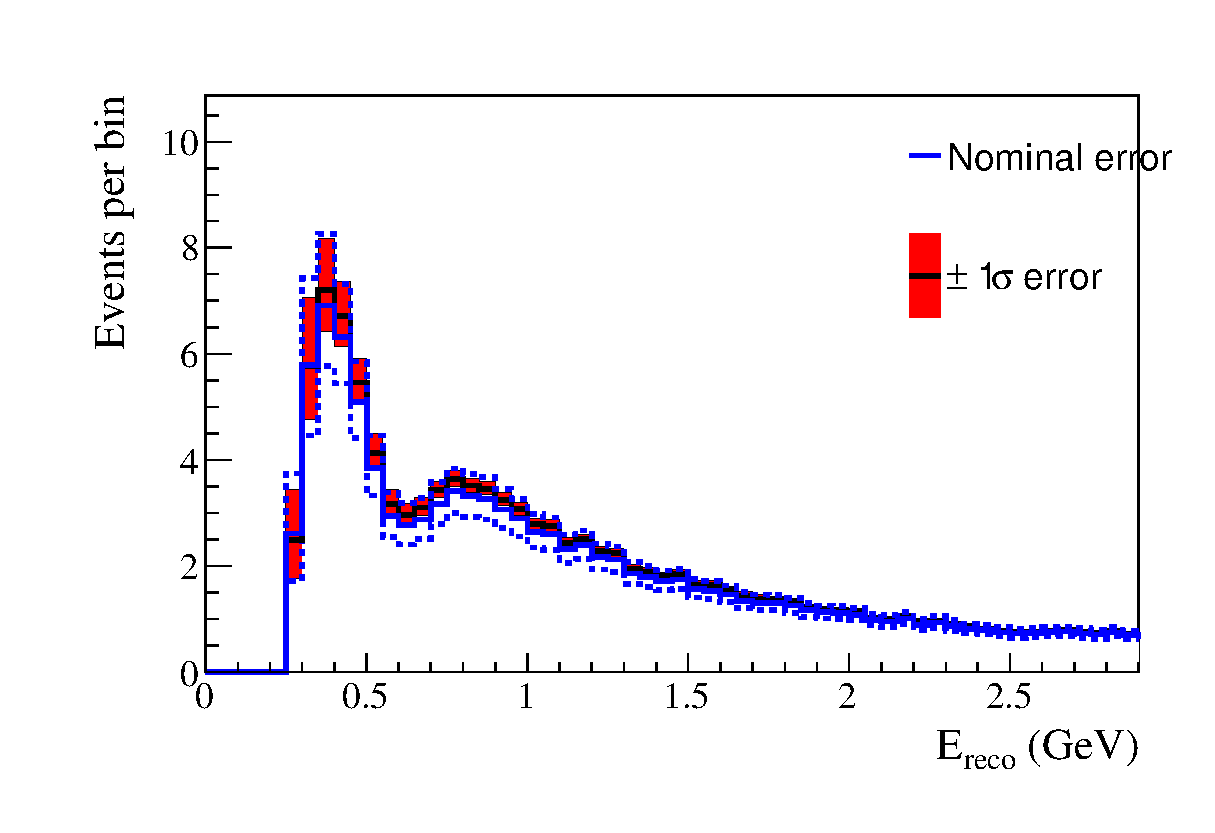
\includegraphics[width=0.9\textwidth]{joint_plots/systematics/Run17c/WithPreBANFF/Asimov_A_1Rmuoscillated_all_envelope.eps} 
\caption{Muon-like, neutrino mode}
\end{subfigure}
\begin{subfigure}[b]{0.49\textwidth} \centering
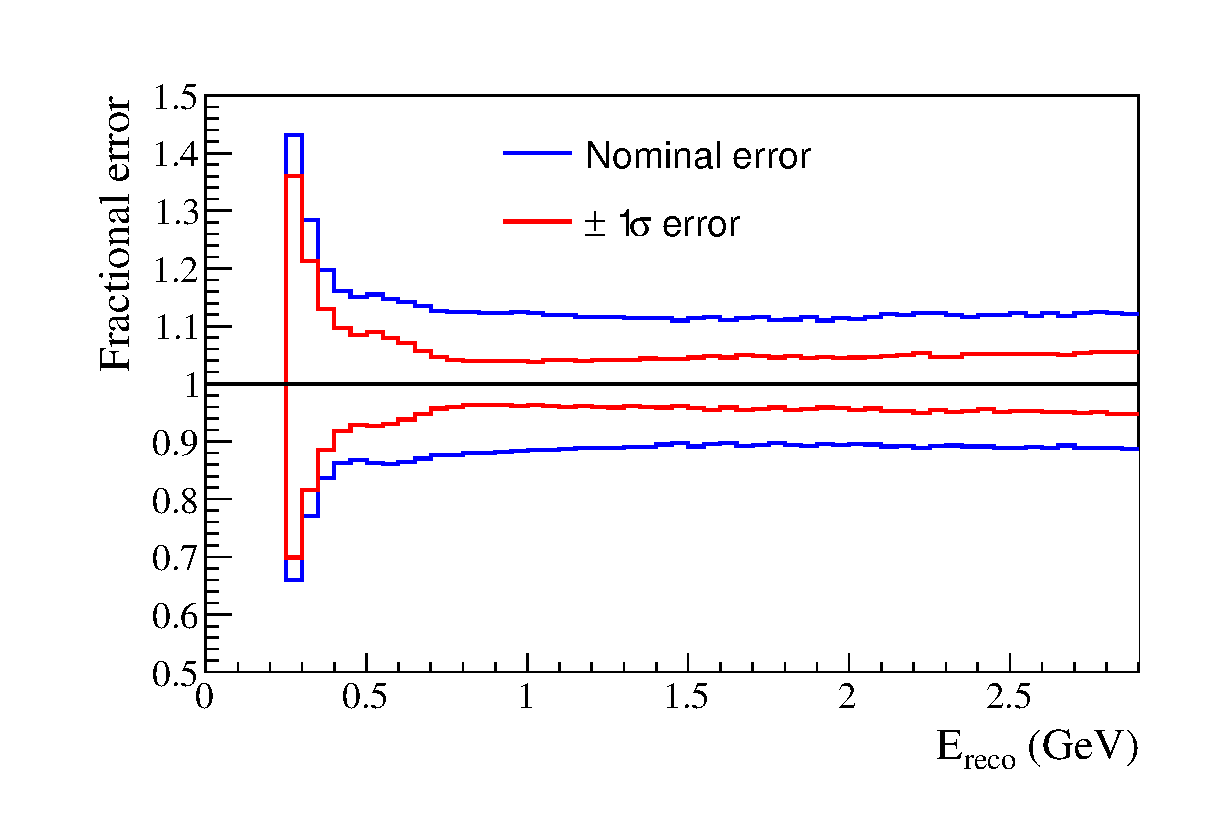
\includegraphics[width=0.9\textwidth]{joint_plots/systematics/Run17c/WithPreBANFF/Asimov_A_1Rmuoscillated_all_envelope_ratio.eps} \\
\caption{Muon-like, neutrino mode}
\end{subfigure}
%rhc mu-like
\begin{subfigure}[b]{0.49\textwidth} \centering
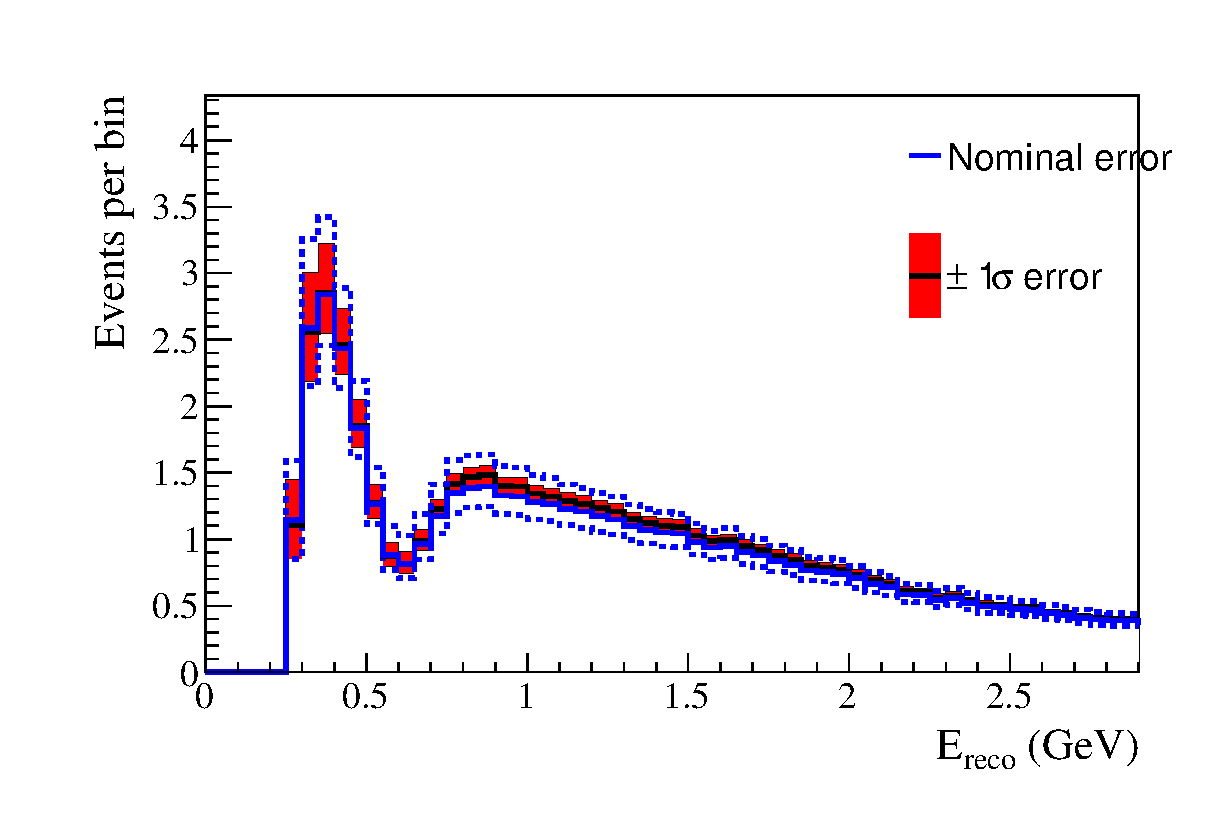
\includegraphics[width=0.9\textwidth]{joint_plots/systematics/Run17c/WithPreBANFF/Asimov_A_RHC1Rmuoscillated_all_envelope.eps} %\\ 
\caption{Muon-like, antineutrino mode}
\end{subfigure}
\begin{subfigure}[b]{0.49\textwidth} \centering
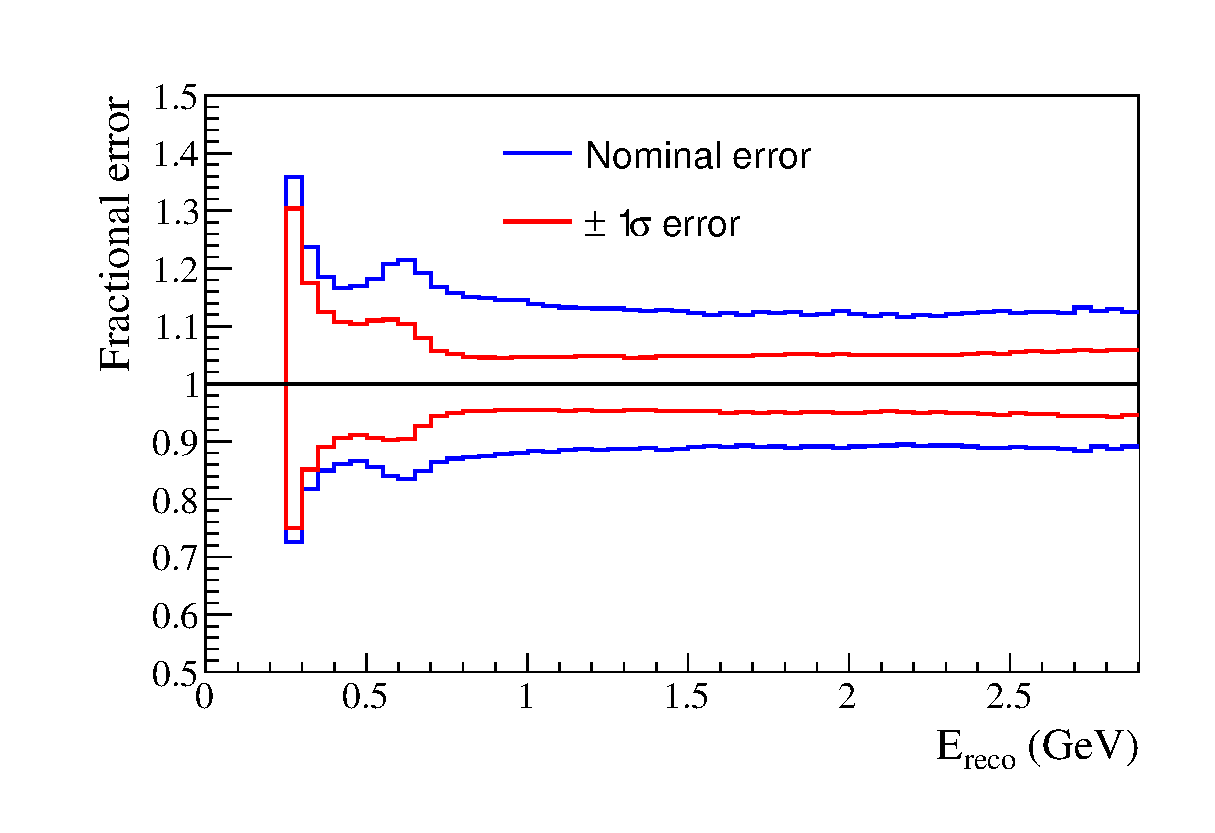
\includegraphics[width=0.9\textwidth]{joint_plots/systematics/Run17c/WithPreBANFF/Asimov_A_RHC1Rmuoscillated_all_envelope_ratio.eps} \\ 
\caption{Muon-like, antineutrino mode}
\end{subfigure}
%fhc e-like
\caption {
Error envelopes (left) and fractional errors (right) for the reconstructed neutrino energy spectrum
for all the systematic parameters.
Both pre- (blue), assuming the CCQE parameters to be gaussian distributed instead of flat, 
and post- (red) BANFF fit errors are shown.
	10k toy MC experiments are generated for the Asimov data set A shown in \cref{tab:osc_params_joint_asimov}
	with random systematic parameters, taking into account their correlations.
	Since the parameters $\delta_{CP}$, $\theta_{23}$ and $\Delta m^2_{32}$ ($\Delta m^2_{13}$) and mass hierarchy
will be measured,
only the uncertainty on 
$\sin^2 \theta_{13}$,
$\sin^2 \theta_{12}$
and 
$\Delta m^2_{21}$ 
are taken into account.
BANFF tuned MC templates are used. 
The distributions correspond to the collected statistics in the full Run 1-7c data set.
The changes due to the Run 1-7c flux and covariance matrix updates are applied.
}
\label{fig:spectra_systematic_Asimov_A_prebanff_run17c_mulike}
\end{figure*}


\begin{figure*}[htb]
\center

\begin{subfigure}[b]{0.49\textwidth} \centering
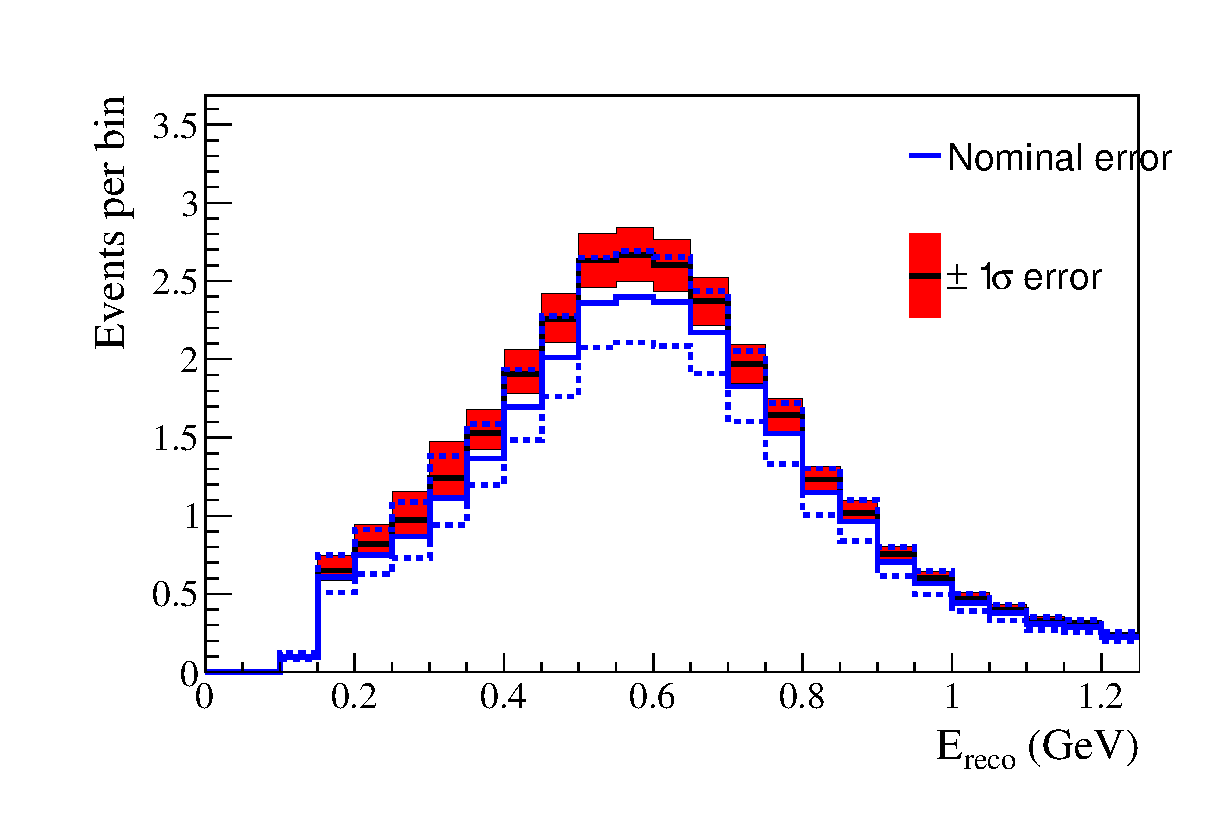
\includegraphics[width=0.9\textwidth]{joint_plots/systematics/Run17c/WithPreBANFF/Asimov_A_1Reoscillated_all_envelope.eps} 
\caption{Electron-like, neutrino mode}
\end{subfigure}
\begin{subfigure}[b]{0.49\textwidth} \centering
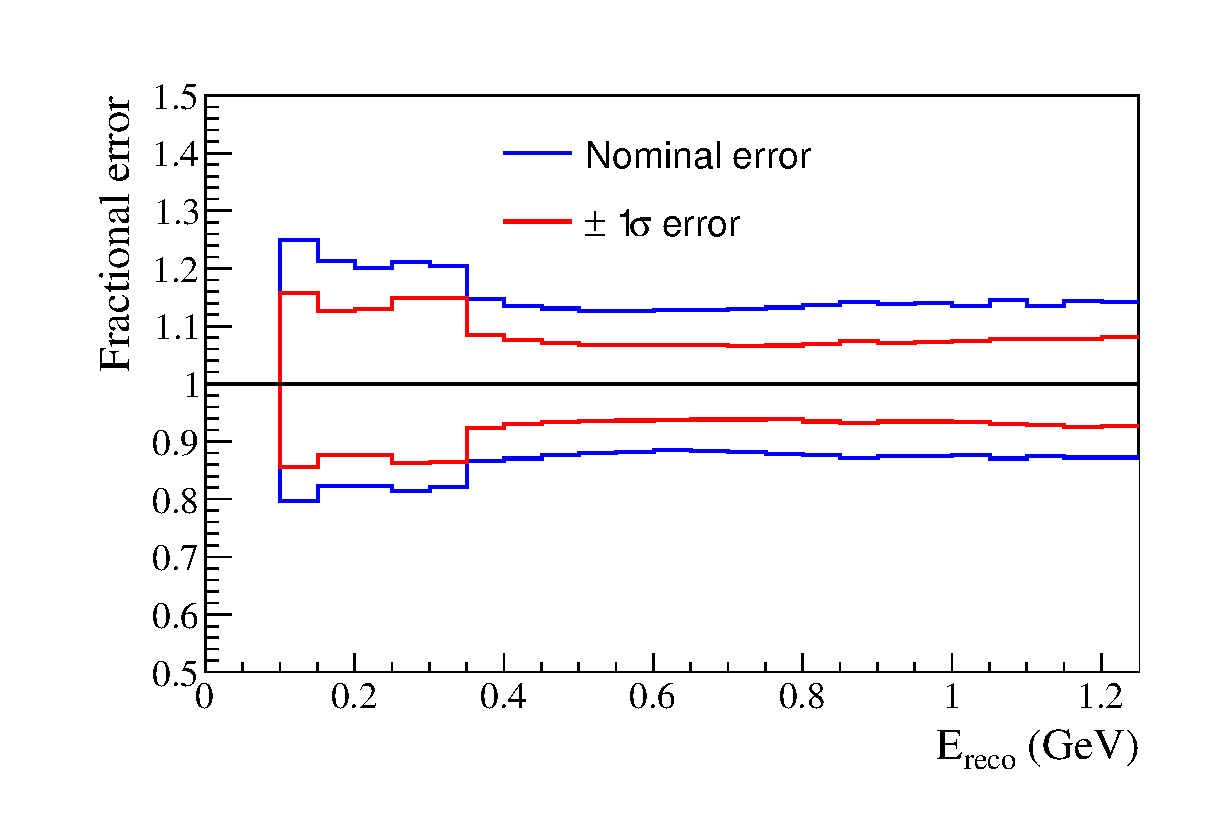
\includegraphics[width=0.9\textwidth]{joint_plots/systematics/Run17c/WithPreBANFF/Asimov_A_1Reoscillated_all_envelope_ratio.eps} 
\caption{Electron-like, neutrino mode}
\end{subfigure}
%rhc e-like
\begin{subfigure}[b]{0.49\textwidth} \centering
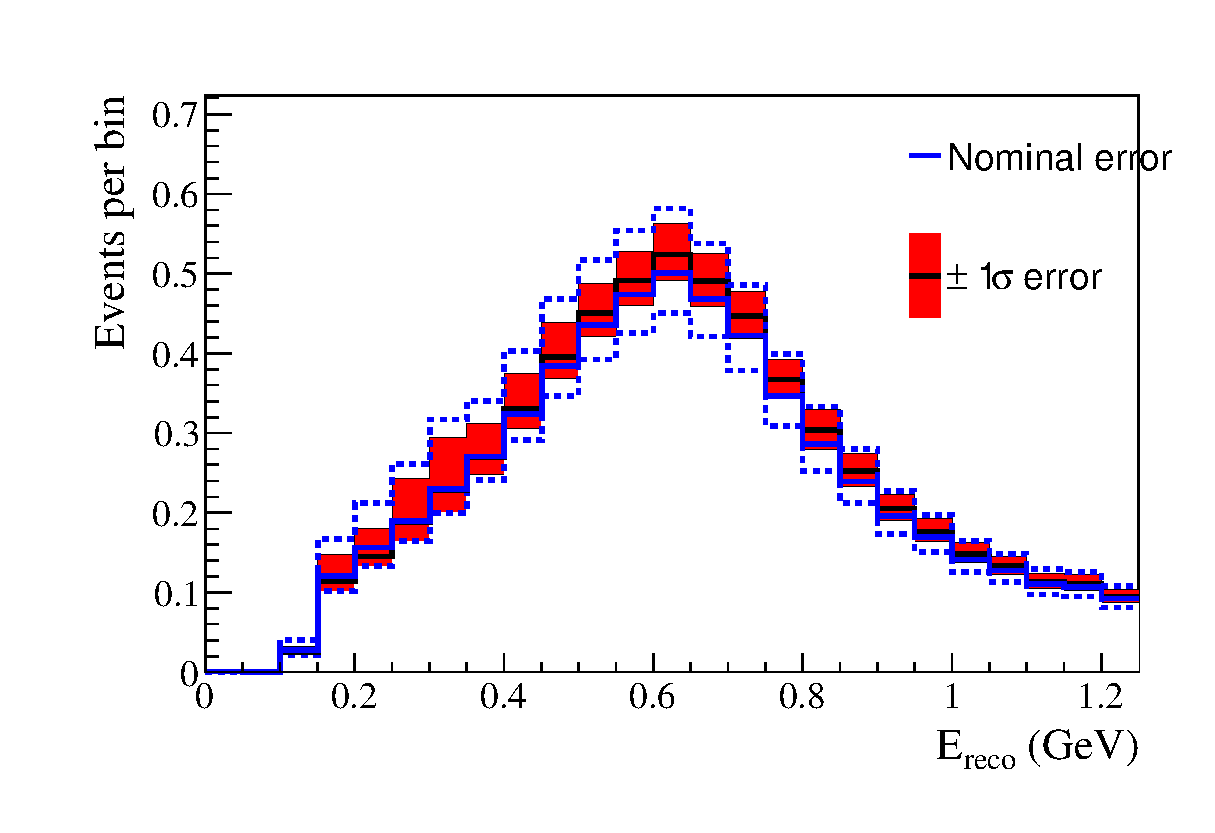
\includegraphics[width=0.9\textwidth]{joint_plots/systematics/Run17c/WithPreBANFF/Asimov_A_RHC1Reoscillated_all_envelope.eps} 
\caption{Electron-like, antineutrino mode}
\end{subfigure}
\begin{subfigure}[b]{0.49\textwidth} \centering
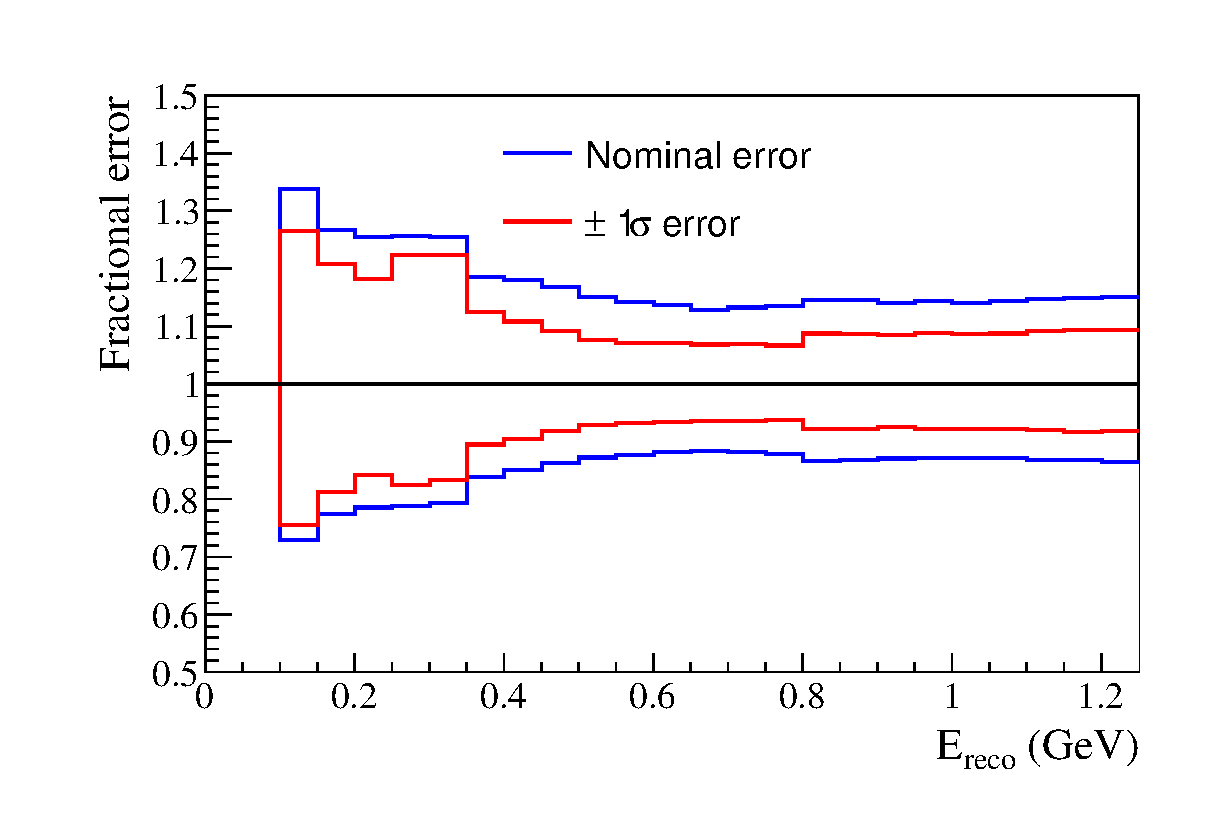
\includegraphics[width=0.9\textwidth]{joint_plots/systematics/Run17c/WithPreBANFF/Asimov_A_RHC1Reoscillated_all_envelope_ratio.eps} 
\caption{Electron-like, antineutrino mode}
\end{subfigure}
%fhc ccpi-like
\begin{subfigure}[b]{0.49\textwidth} \centering
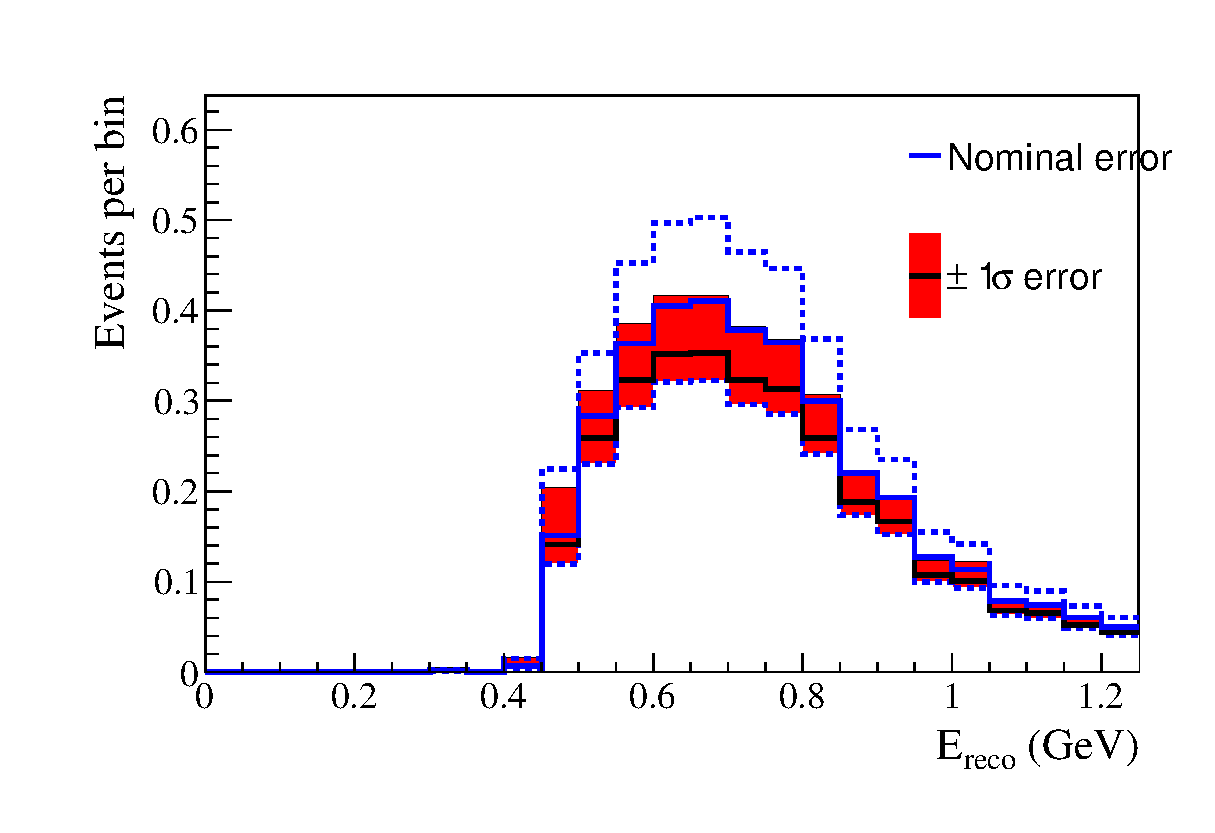
\includegraphics[width=0.9\textwidth]{joint_plots/systematics/Run17c/WithPreBANFF/Asimov_A_MultiReoscillated_all_envelope.eps} 
\caption{\nueCConepi{}, neutrino mode}
\end{subfigure}
\begin{subfigure}[b]{0.49\textwidth} \centering
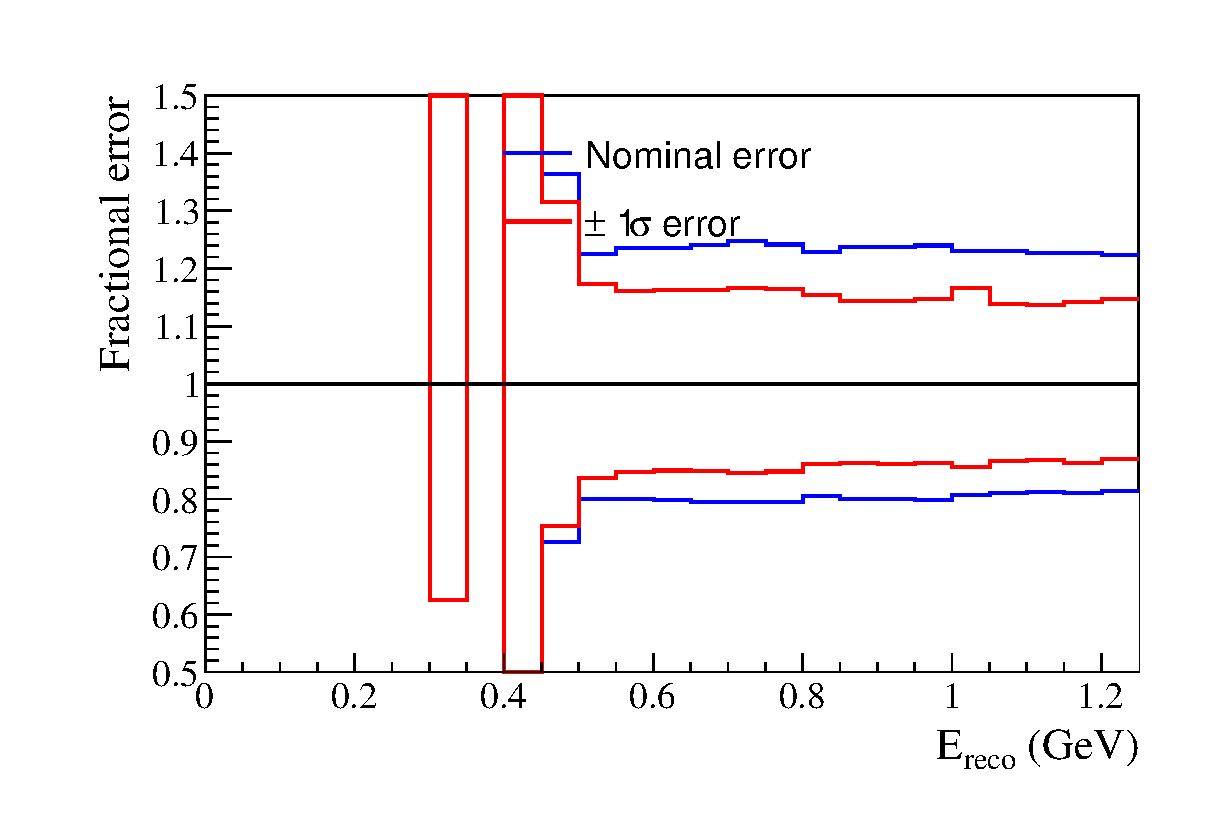
\includegraphics[width=0.9\textwidth]{joint_plots/systematics/Run17c/WithPreBANFF/Asimov_A_MultiReoscillated_all_envelope_ratio.eps} 
\caption{\nueCConepi{}, neutrino mode}
\end{subfigure}
\caption {
Error envelopes (left) and fractional errors (right) for the reconstructed neutrino energy spectrum
for all the systematic parameters.
Both pre- (blue), assuming the CCQE parameters to be gaussian distributed instead of flat, 
and post- (red) BANFF fit errors are shown.
10k toy MC experiments are generated for the Asimov data set A shown in \cref{tab:osc_params_joint_asimov}
with randomised systematic parameters, taking into account their correlations.
Since the parameters $\delta_{CP}$, $\theta_{23}$ and $\Delta m^2_{32}$ ($\Delta m^2_{13}$) and mass hierarchy
will be measured,
only the uncertainty on 
$\sin^2 \theta_{13}$,
$\sin^2 \theta_{12}$
and 
$\Delta m^2_{21}$ 
are taken into account.
BANFF tuned MC templates are used. 
The distributions correspond to the collected statistics in the full Run 1-7c data set.
The changes due to the Run 1-7c flux and covariance matrix updates are applied.
}
\label{fig:spectra_systematic_Asimov_A_prebanff_run17c_elike}
\end{figure*}




\begin{figure*}[htb]
\center
%fhc mu-like
\begin{subfigure}[b]{0.49\textwidth} \centering
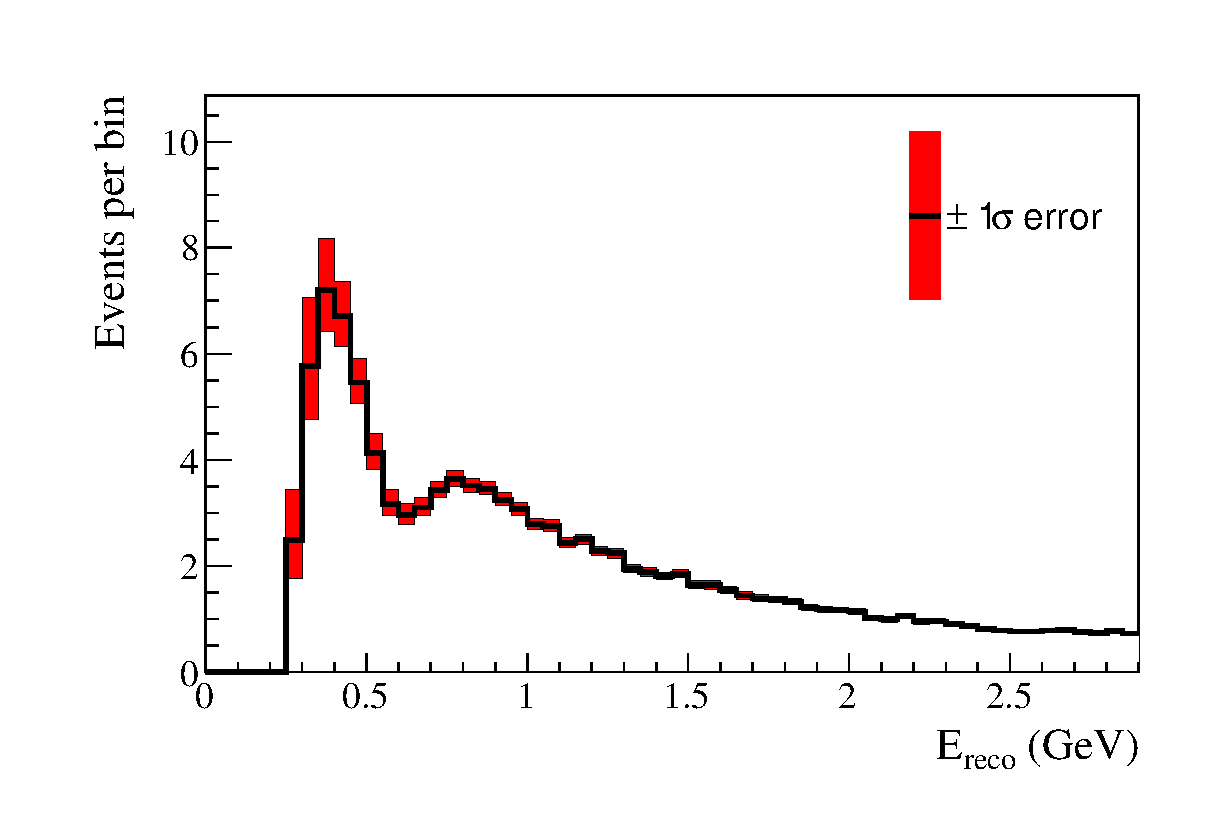
\includegraphics[width=0.9\textwidth]{joint_plots/systematics/Run17c/Asimov_A_1Rmuoscillated_all_envelope.eps} 
\caption{Muon-like, neutrino mode}
\end{subfigure}
\begin{subfigure}[b]{0.49\textwidth} \centering
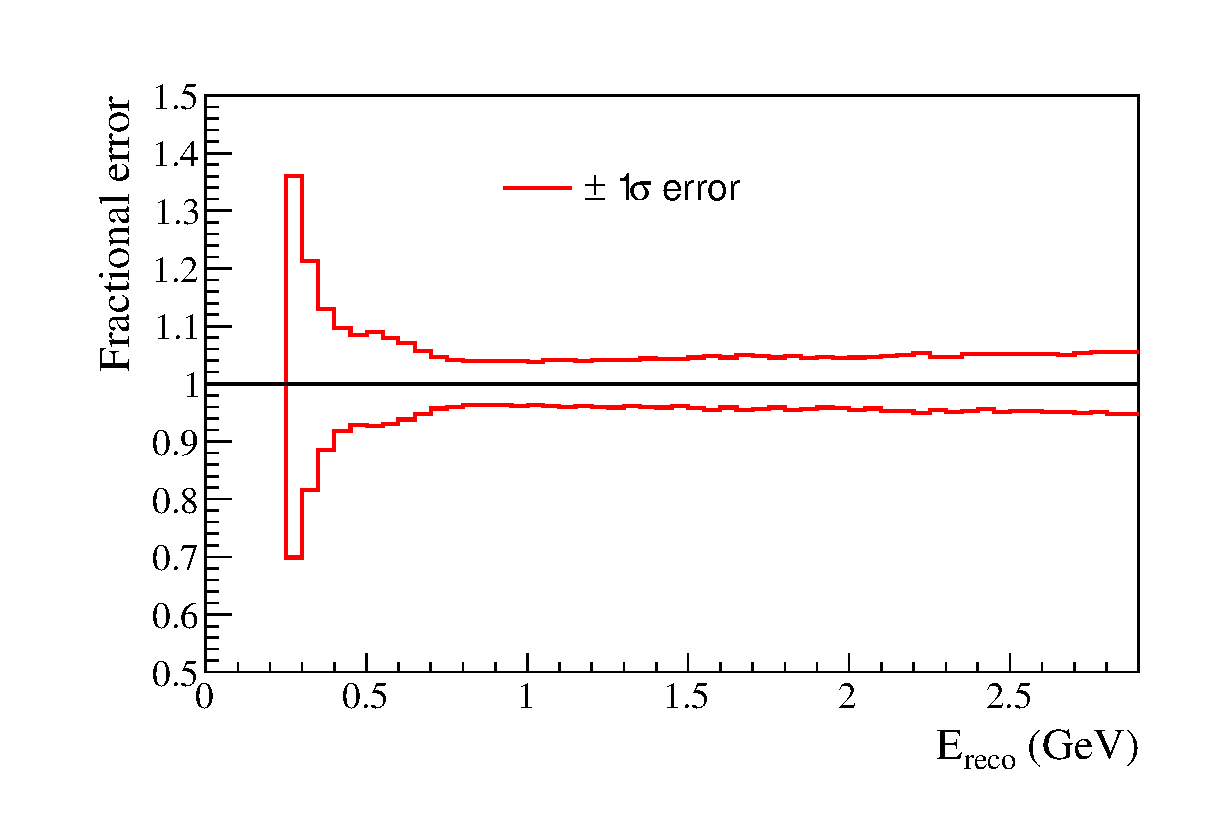
\includegraphics[width=0.9\textwidth]{joint_plots/systematics/Run17c/Asimov_A_1Rmuoscillated_all_envelope_ratio.eps} \\
\caption{Muon-like, neutrino mode}
\end{subfigure}
%rhc mu-like
\begin{subfigure}[b]{0.49\textwidth} \centering
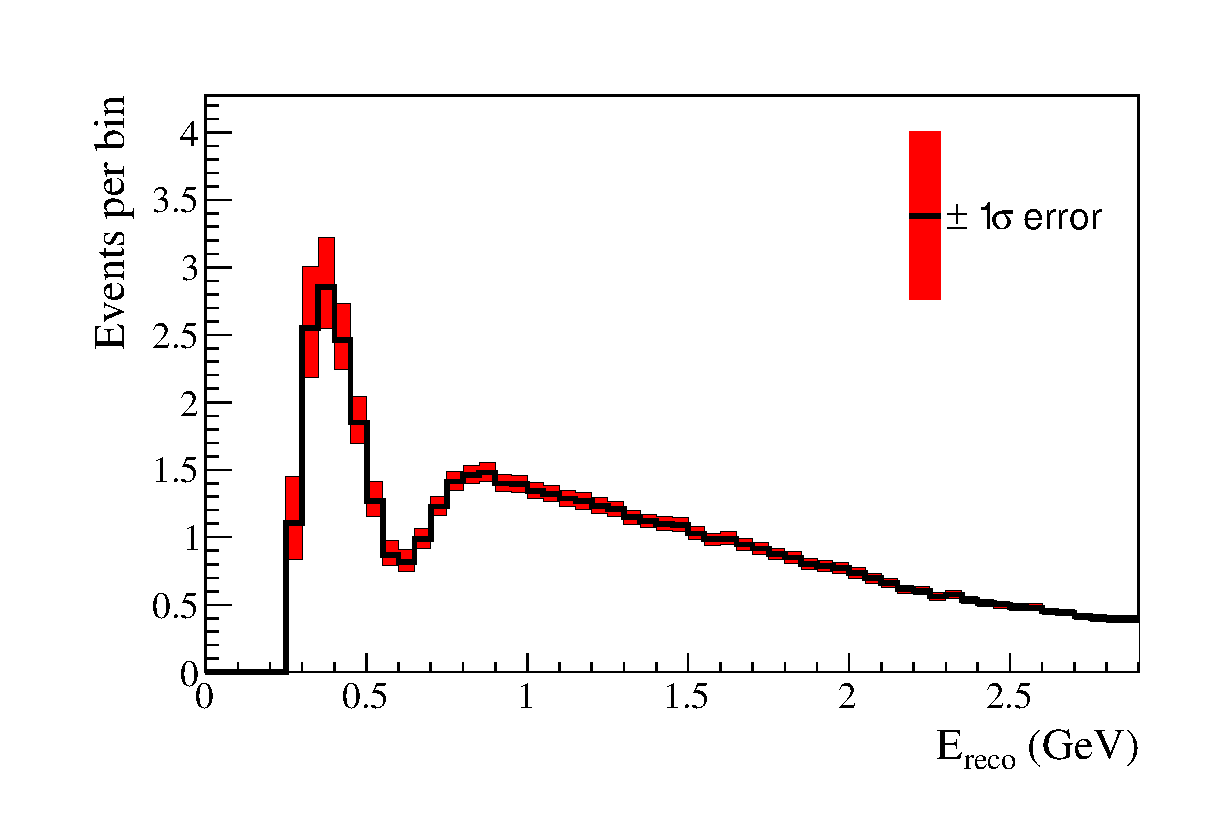
\includegraphics[width=0.9\textwidth]{joint_plots/systematics/Run17c/Asimov_A_RHC1Rmuoscillated_all_envelope.eps} %\\ 
\caption{Muon-like, antineutrino mode}
\end{subfigure}
\begin{subfigure}[b]{0.49\textwidth} \centering
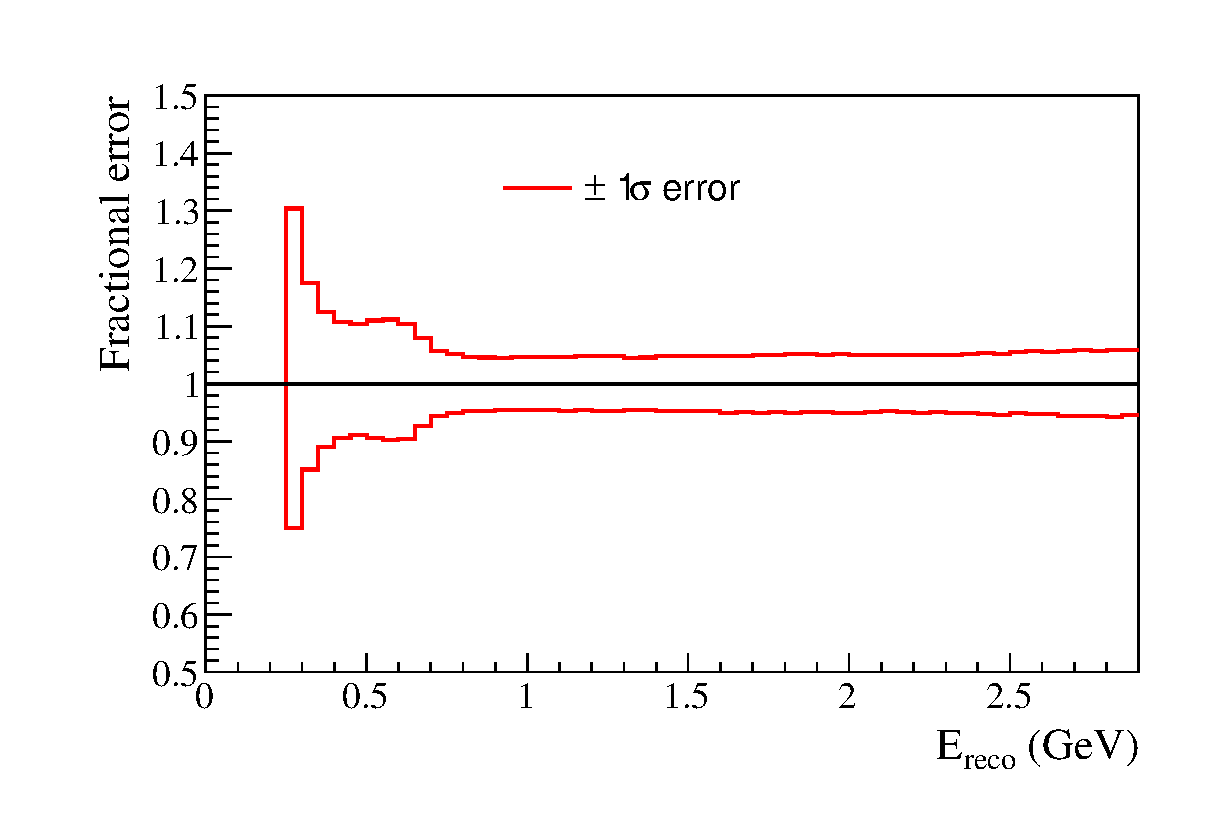
\includegraphics[width=0.9\textwidth]{joint_plots/systematics/Run17c/Asimov_A_RHC1Rmuoscillated_all_envelope_ratio.eps} \\ 
\caption{Muon-like, antineutrino mode}
\end{subfigure}
%fhc e-like
\caption {
Error envelopes (left) and fractional errors (right) for the reconstructed neutrino energy spectrum
for all the systematic parameters.
	10k toy MC experiments are generated for the Asimov data set A shown in \cref{tab:osc_params_joint_asimov}
	with random systematic parameters, taking into account their correlations.
	Since the parameters $\delta_{CP}$, $\theta_{23}$ and $\Delta m^2_{32}$ ($\Delta m^2_{13}$) and mass hierarchy
will be measured,
only the uncertainty on 
$\sin^2 \theta_{13}$,
$\sin^2 \theta_{12}$
and 
$\Delta m^2_{21}$ 
are taken into account.
BANFF tuned MC templates are used. 
The distributions correspond to the collected statistics in the full Run 1-7c data set.
The changes due to the Run 1-7c flux and covariance matrix updates are applied.
}
\label{fig:spectra_systematic_Asimov_A_run17c_mulike}
\end{figure*}


\begin{figure*}[htb]
\center

\begin{subfigure}[b]{0.49\textwidth} \centering
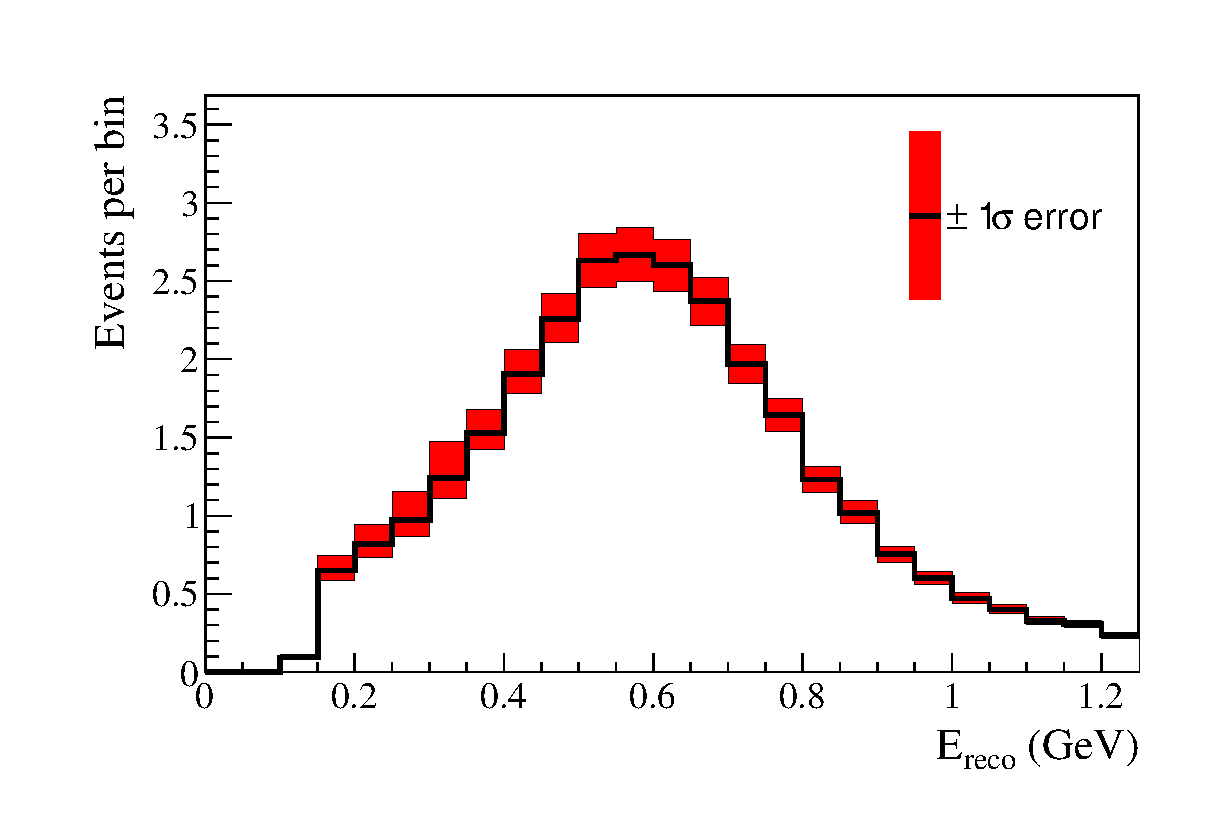
\includegraphics[width=0.9\textwidth]{joint_plots/systematics/Run17c/Asimov_A_1Reoscillated_all_envelope.eps} 
\caption{Electron-like, neutrino mode}
\end{subfigure}
\begin{subfigure}[b]{0.49\textwidth} \centering
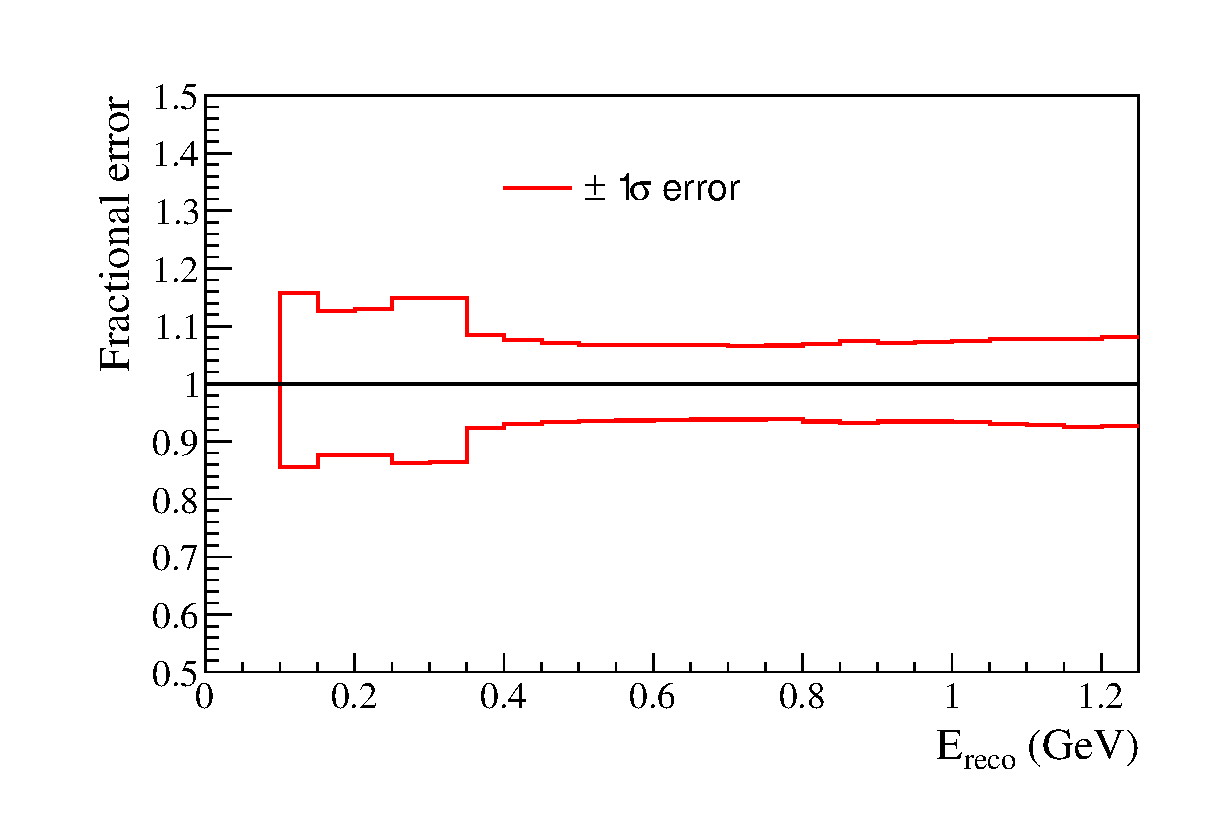
\includegraphics[width=0.9\textwidth]{joint_plots/systematics/Run17c/Asimov_A_1Reoscillated_all_envelope_ratio.eps} 
\caption{Electron-like, neutrino mode}
\end{subfigure}
%rhc e-like
\begin{subfigure}[b]{0.49\textwidth} \centering
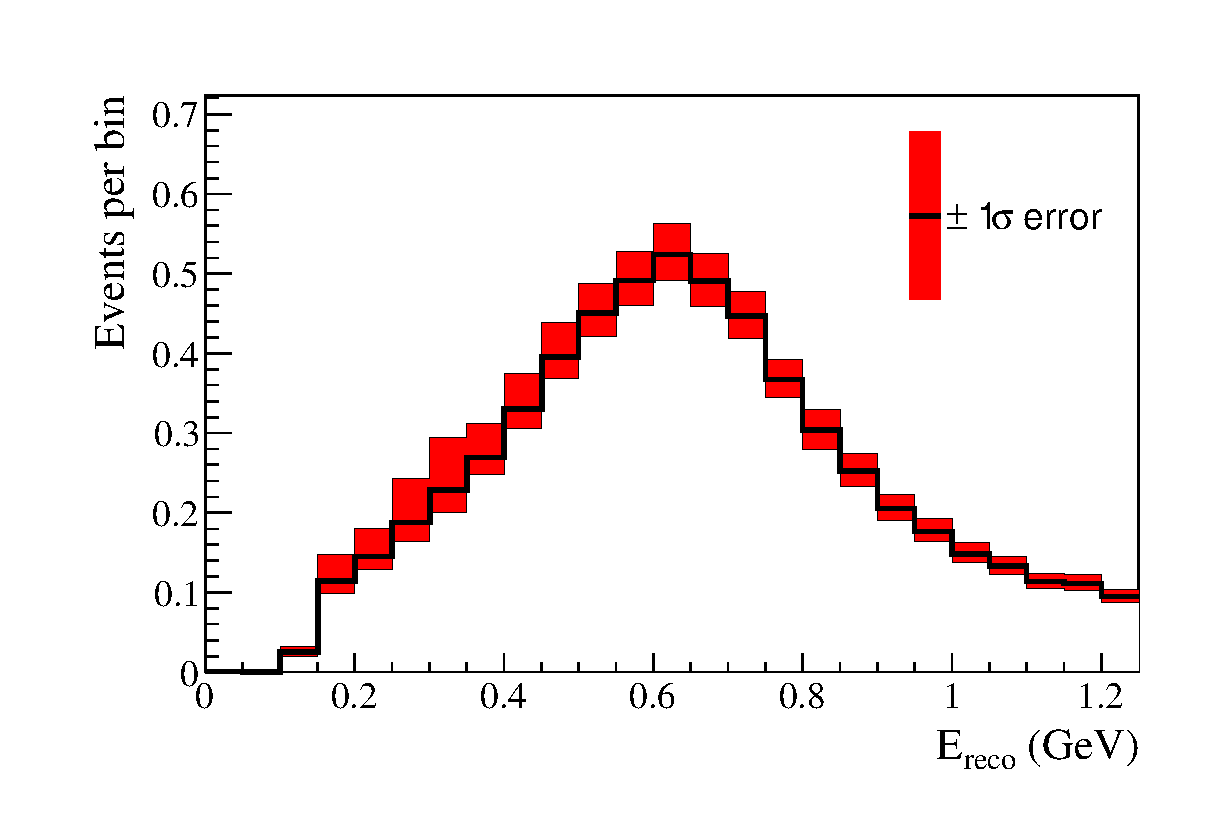
\includegraphics[width=0.9\textwidth]{joint_plots/systematics/Run17c/Asimov_A_RHC1Reoscillated_all_envelope.eps} 
\caption{Electron-like, antineutrino mode}
\end{subfigure}
\begin{subfigure}[b]{0.49\textwidth} \centering
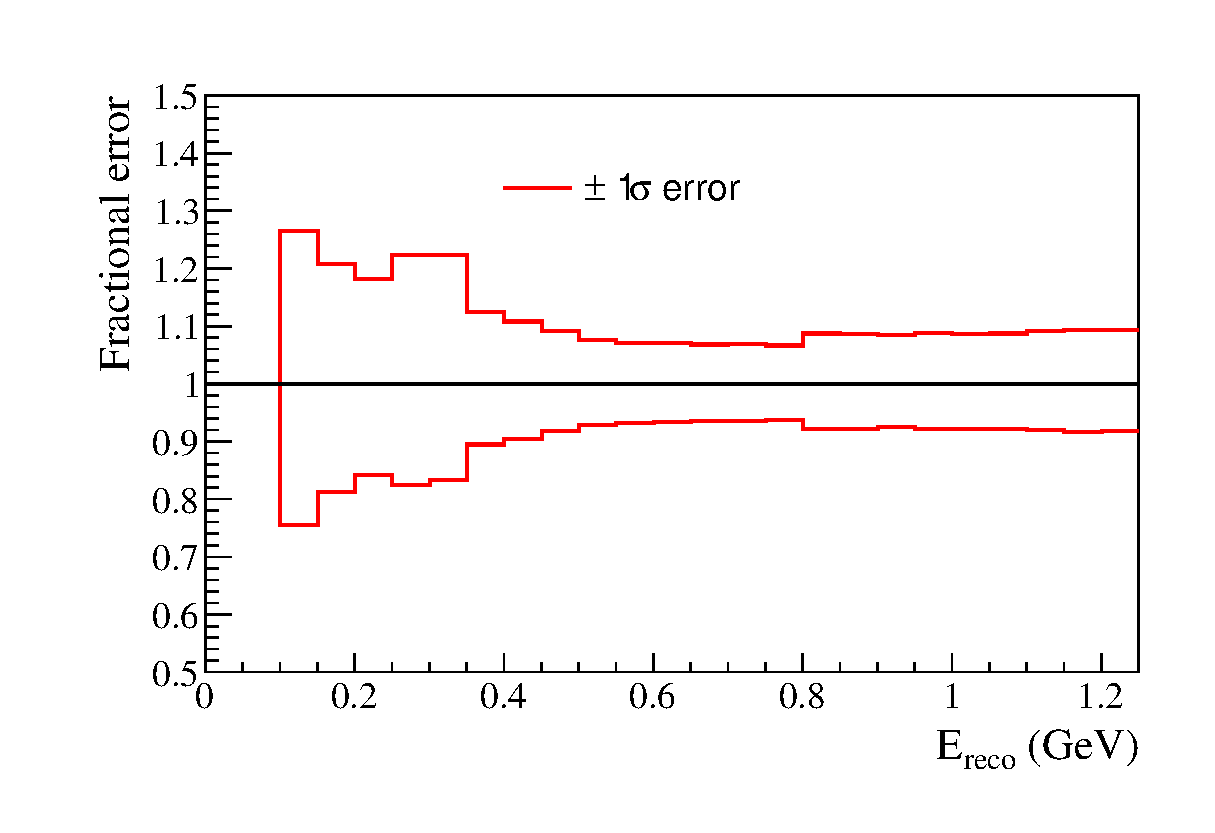
\includegraphics[width=0.9\textwidth]{joint_plots/systematics/Run17c/Asimov_A_RHC1Reoscillated_all_envelope_ratio.eps} 
\caption{Electron-like, antineutrino mode}
\end{subfigure}
%fhc e-like
\begin{subfigure}[b]{0.49\textwidth} \centering
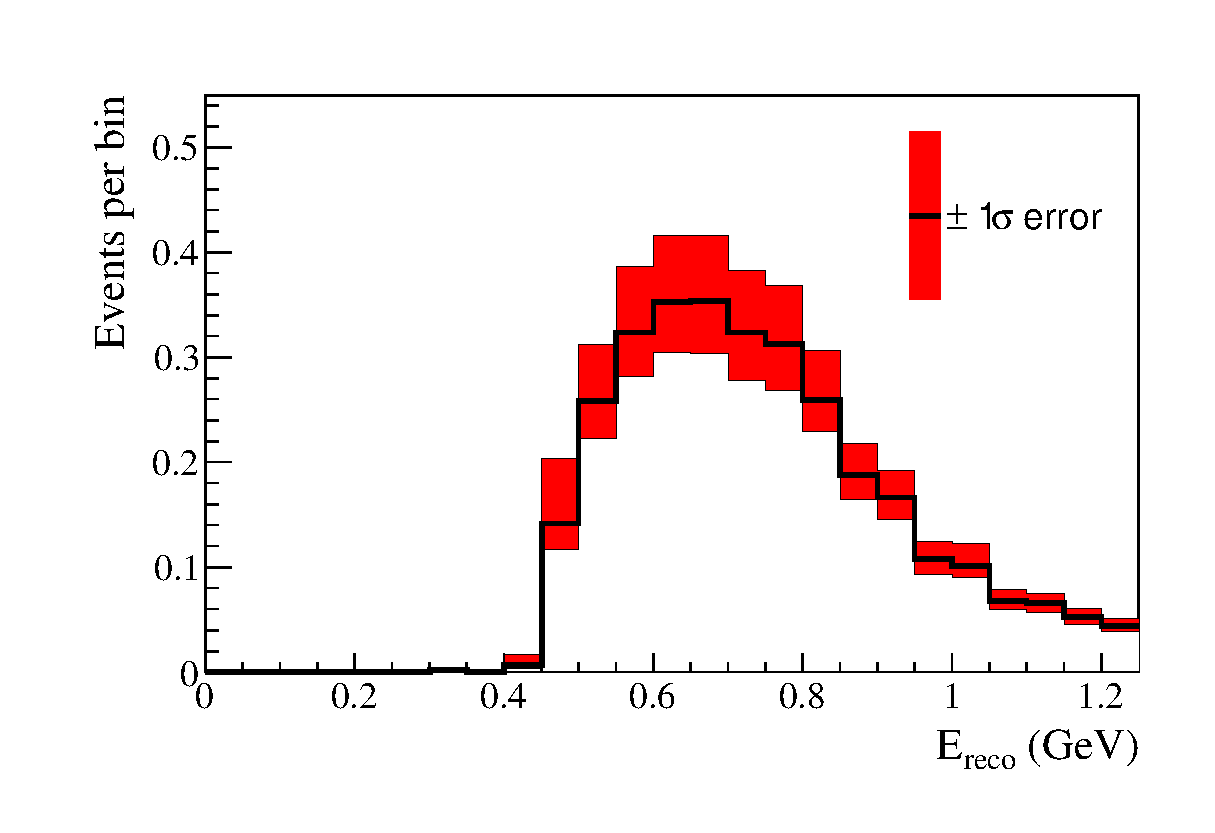
\includegraphics[width=0.9\textwidth]{joint_plots/systematics/Run17c/Asimov_A_MultiReoscillated_all_envelope.eps} 
\caption{\nueCConepi{}, neutrino mode}
\end{subfigure}
\begin{subfigure}[b]{0.49\textwidth} \centering
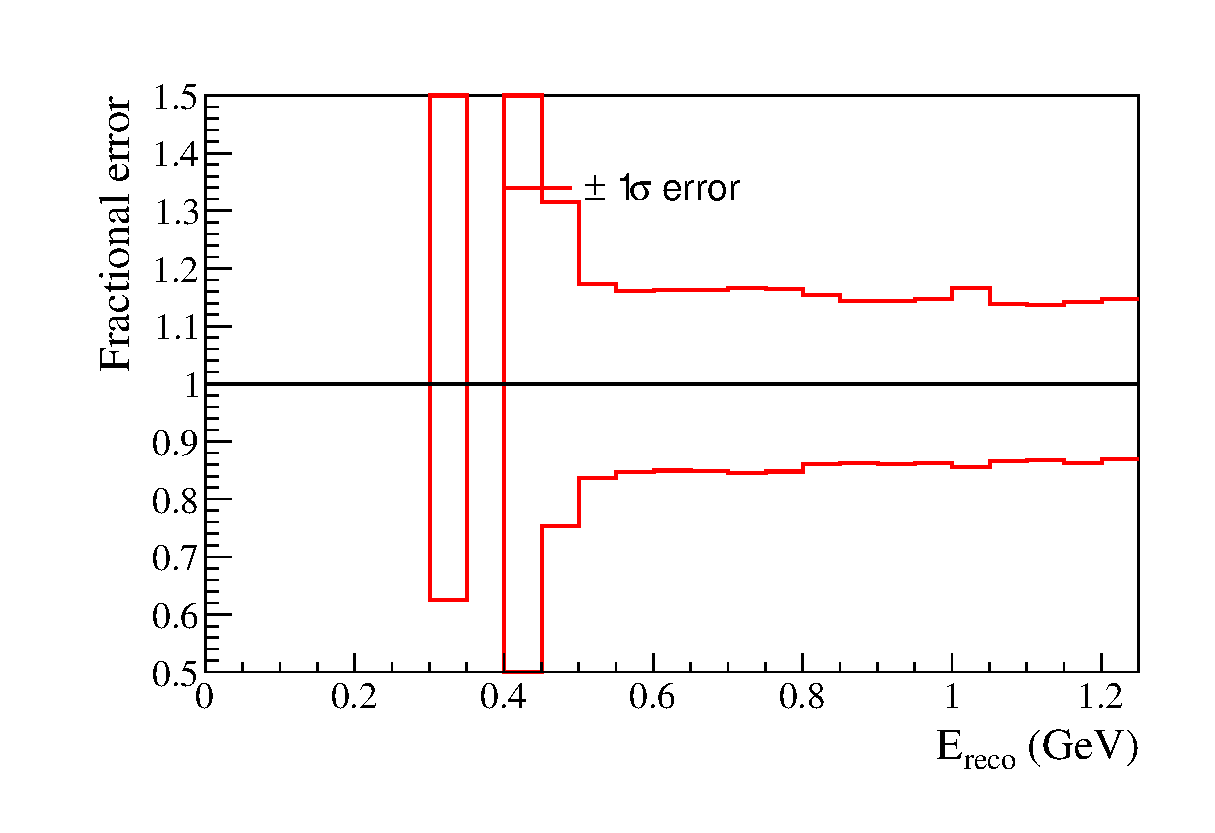
\includegraphics[width=0.9\textwidth]{joint_plots/systematics/Run17c/Asimov_A_MultiReoscillated_all_envelope_ratio.eps} 
\caption{\nueCConepi{}, neutrino mode}
\end{subfigure}
\caption {
Error envelopes (left) and fractional errors (right) for the reconstructed neutrino energy spectrum
for all the systematic parameters.
10k toy MC experiments are generated for the Asimov data set A shown in \cref{tab:osc_params_joint_asimov}
with randomised systematic parameters, taking into account their correlations.
Since the parameters $\delta_{CP}$, $\theta_{23}$ and $\Delta m^2_{32}$ ($\Delta m^2_{13}$) and mass hierarchy
will be measured,
only the uncertainty on 
$\sin^2 \theta_{13}$,
$\sin^2 \theta_{12}$
and 
$\Delta m^2_{21}$ 
are taken into account.
BANFF tuned MC templates are used. 
The distributions correspond to the collected statistics in the full Run 1-7c data set.
The changes due to the Run 1-7c flux and covariance matrix updates are applied.
}
\label{fig:spectra_systematic_Asimov_A_run17c_elike}
\end{figure*}



%%%% Single systematic sources of Asimov A


\begin{figure*}[htb]
\center
%fhc mu-like
\begin{subfigure}[b]{0.49\textwidth} \centering
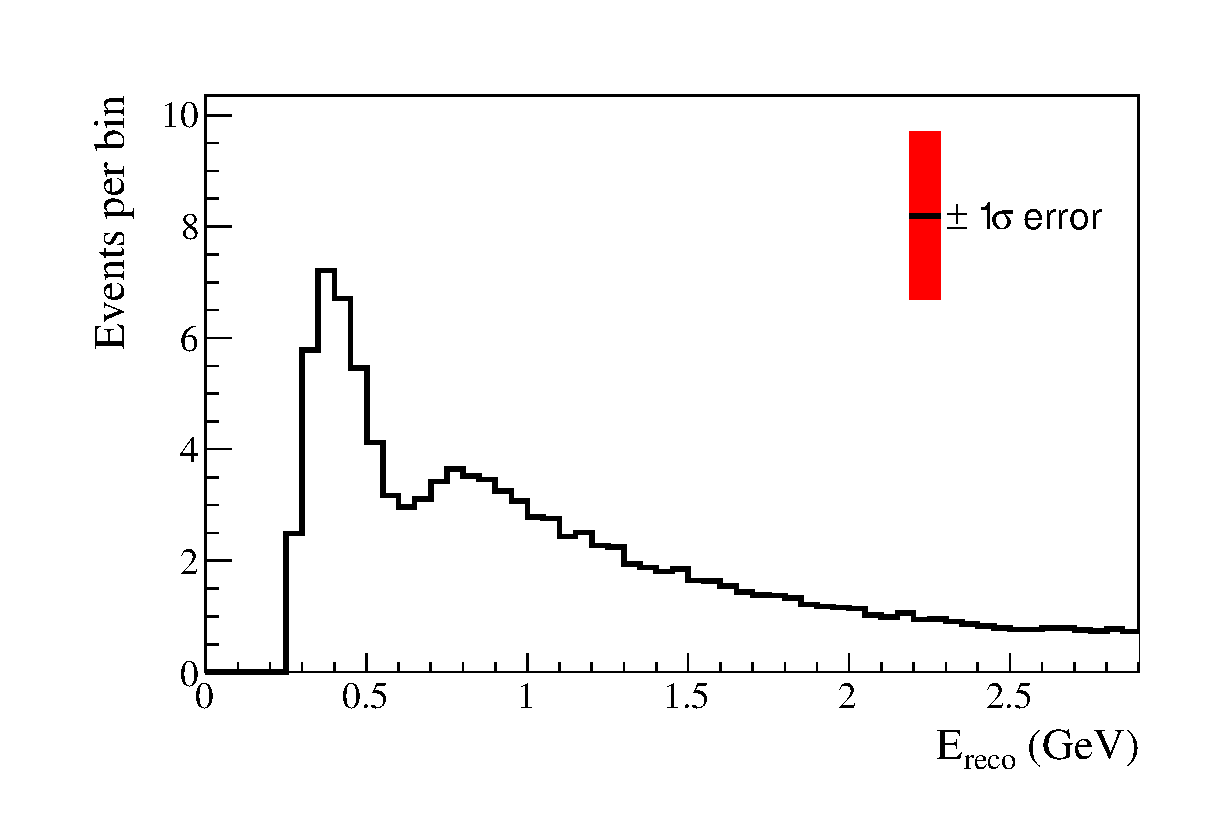
\includegraphics[width=0.9\textwidth]{joint_plots/systematics/Run17c/Asimov_A_1Rmuoscillated_Osc_param_envelope.eps}
\caption{Muon-like, neutrino mode}
\end{subfigure}
\begin{subfigure}[b]{0.49\textwidth} \centering
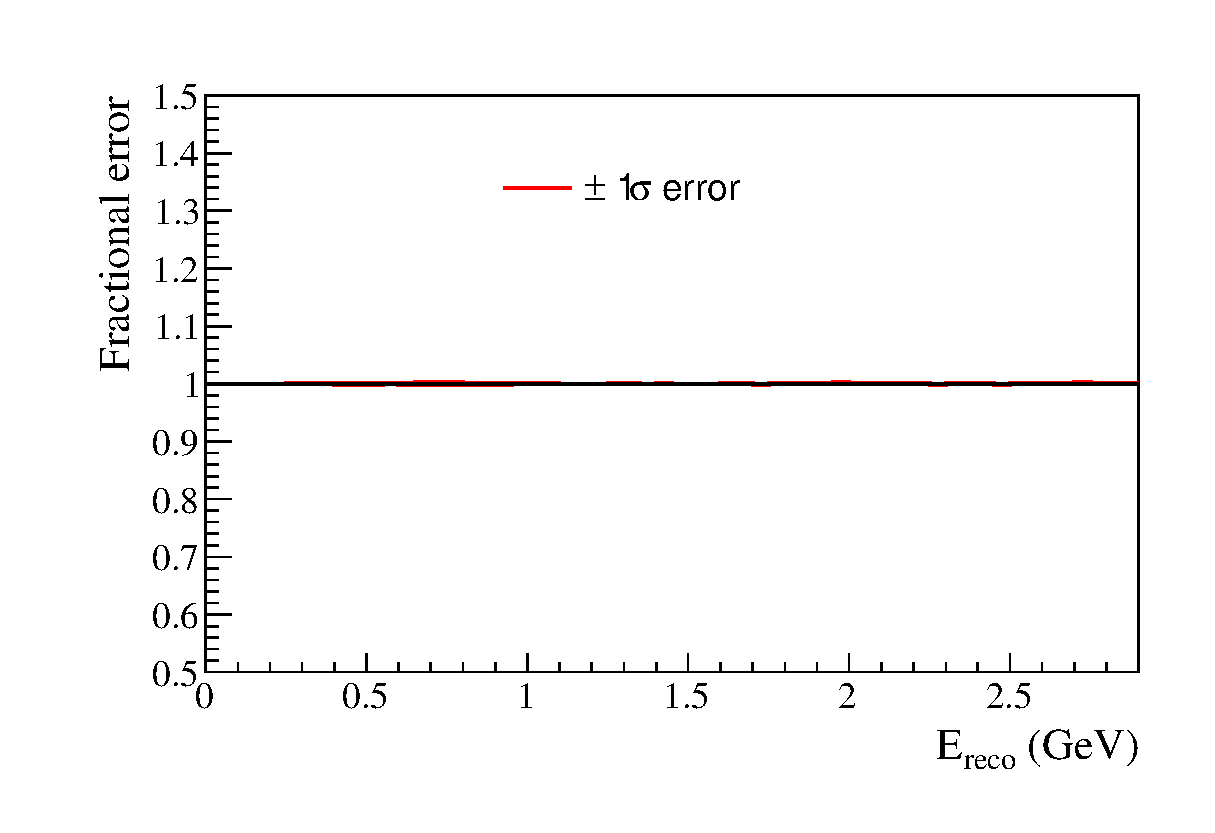
\includegraphics[width=0.9\textwidth]{joint_plots/systematics/Run17c/Asimov_A_1Rmuoscillated_Osc_param_envelope_ratio.eps} 
\caption{Muon-like, neutrino mode}
\end{subfigure}
%rhc mu-like
\begin{subfigure}[b]{0.49\textwidth} \centering
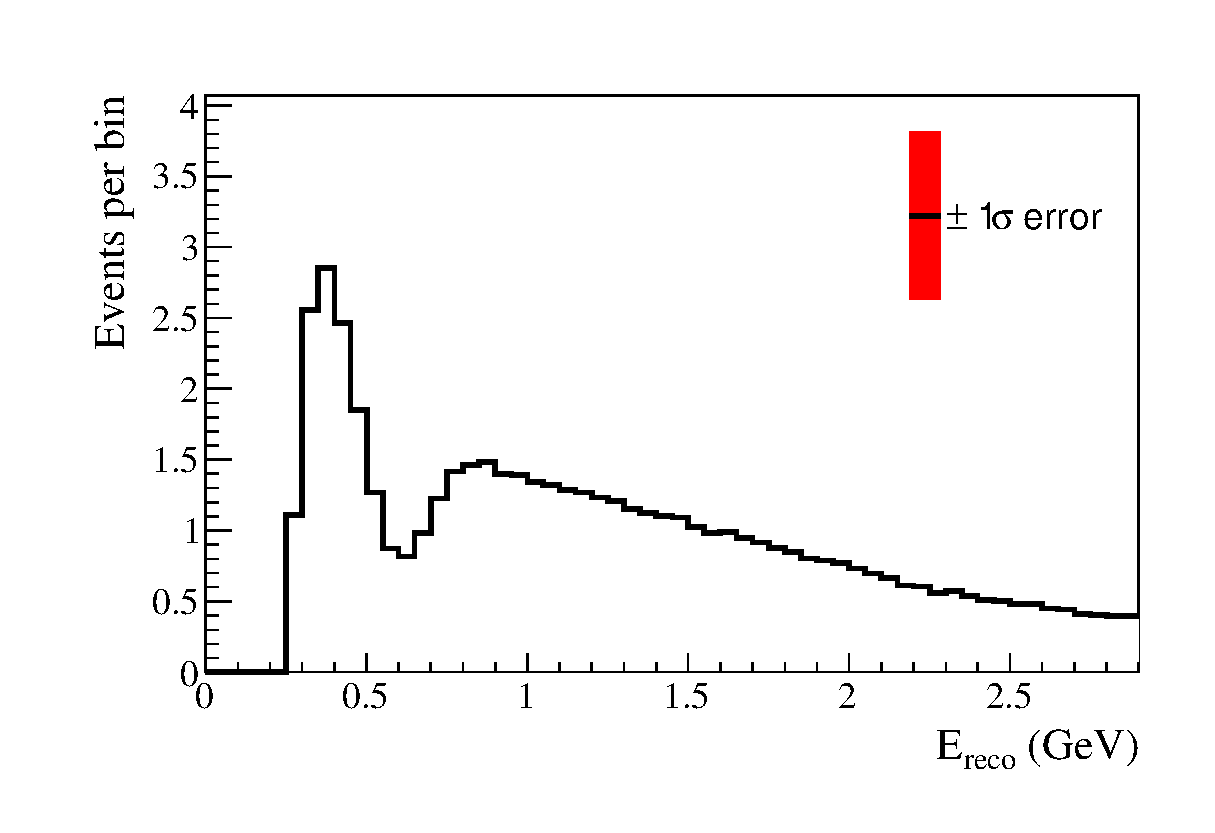
\includegraphics[width=0.9\textwidth]{joint_plots/systematics/Run17c/Asimov_A_RHC1Rmuoscillated_Osc_param_envelope.eps} \\ 
\caption{Muon-like, antineutrino mode}
\end{subfigure}
\begin{subfigure}[b]{0.49\textwidth} \centering
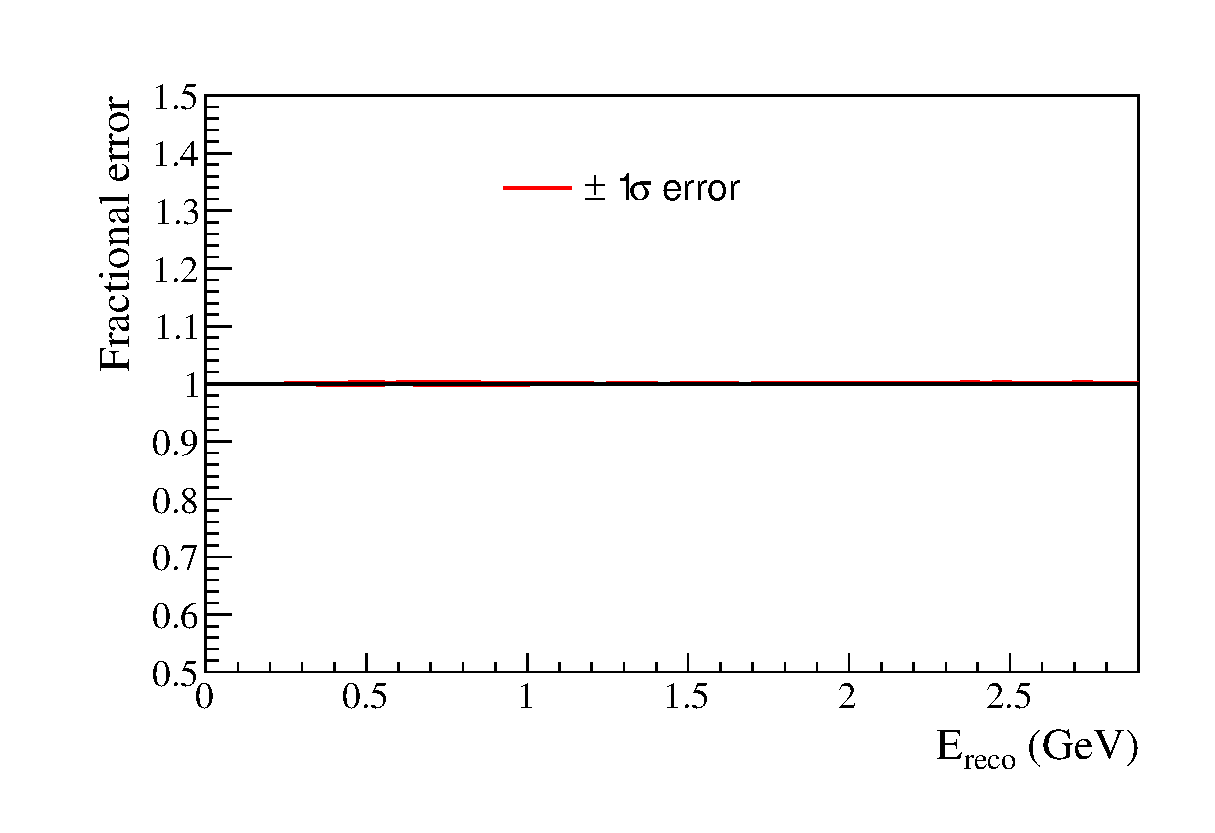
\includegraphics[width=0.9\textwidth]{joint_plots/systematics/Run17c/Asimov_A_RHC1Rmuoscillated_Osc_param_envelope_ratio.eps} \\ 
\caption{Muon-like, antineutrino mode}
\end{subfigure}
%fhc e-like
\caption {
Error envelopes (left) and fractional errors (right) for the reconstructed neutrino energy spectrum
as a result of the oscillation systematic parameters.
	10k toy MC experiments are generated for the Asimov data set A shown in \cref{tab:osc_params_joint_asimov}
	with random systematic parameters, taking into account their correlations.
	Since the parameters $\delta_{CP}$, $\theta_{23}$ and $\Delta m^2_{32}$ ($\Delta m^2_{13}$) and mass hierarchy
will be measured,
only the uncertainty on 
$\sin^2 \theta_{13}$,
$\sin^2 \theta_{12}$
and 
$\Delta m^2_{21}$ 
are taken into account.
BANFF tuned MC templates are used. 
The distributions correspond to the collected statistics in the full Run 1-7c data set.
The changes due to the Run 1-7c flux and covariance matrix updates are applied.
}
\label{fig:Osc_envelope_Asimov_A_run17c_mulike}
\end{figure*}


\begin{figure*}[htb]
\center

\begin{subfigure}[b]{0.49\textwidth} \centering
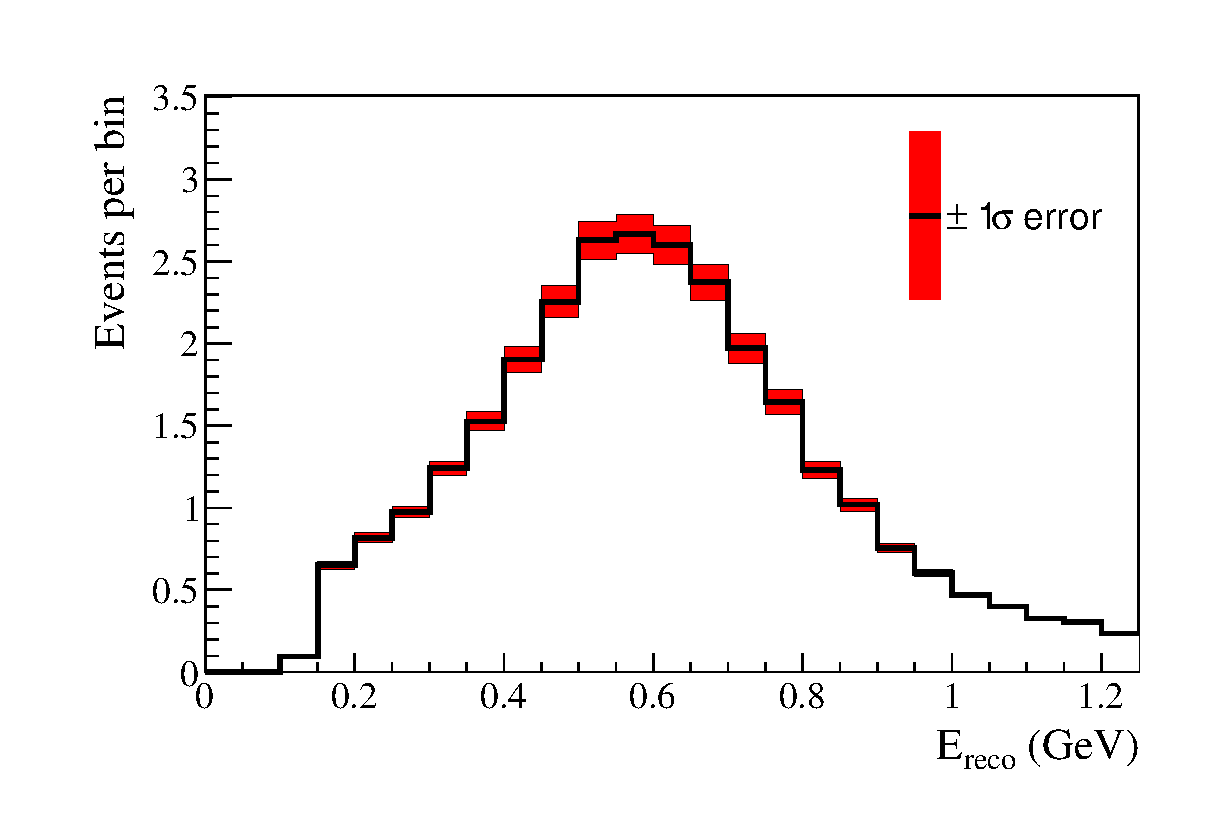
\includegraphics[width=0.9\textwidth]{joint_plots/systematics/Run17c/Asimov_A_1Reoscillated_Osc_param_envelope.eps} 
\caption{Electron-like, neutrino mode}
\end{subfigure}
\begin{subfigure}[b]{0.49\textwidth} \centering
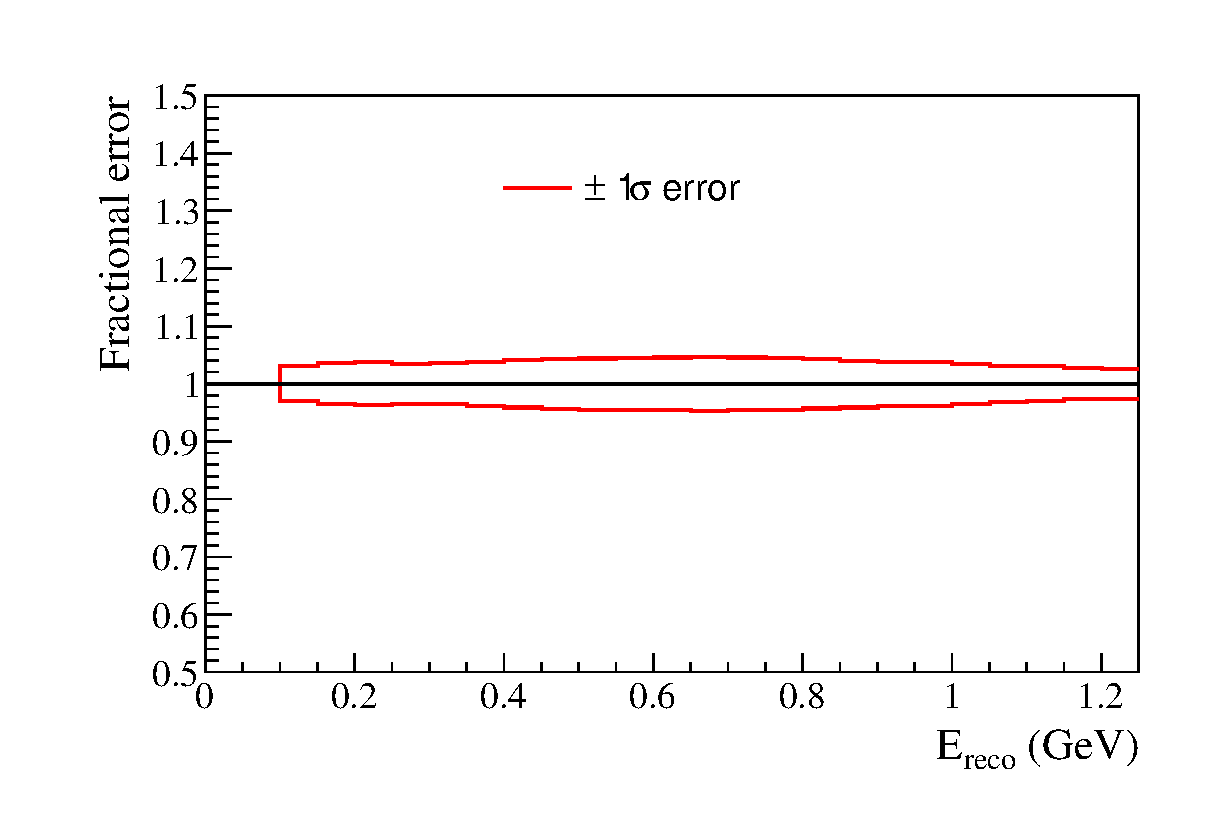
\includegraphics[width=0.9\textwidth]{joint_plots/systematics/Run17c/Asimov_A_1Reoscillated_Osc_param_envelope_ratio.eps}
\caption{Electron-like, neutrino mode}
\end{subfigure}
%rhc e-like
\begin{subfigure}[b]{0.49\textwidth} \centering
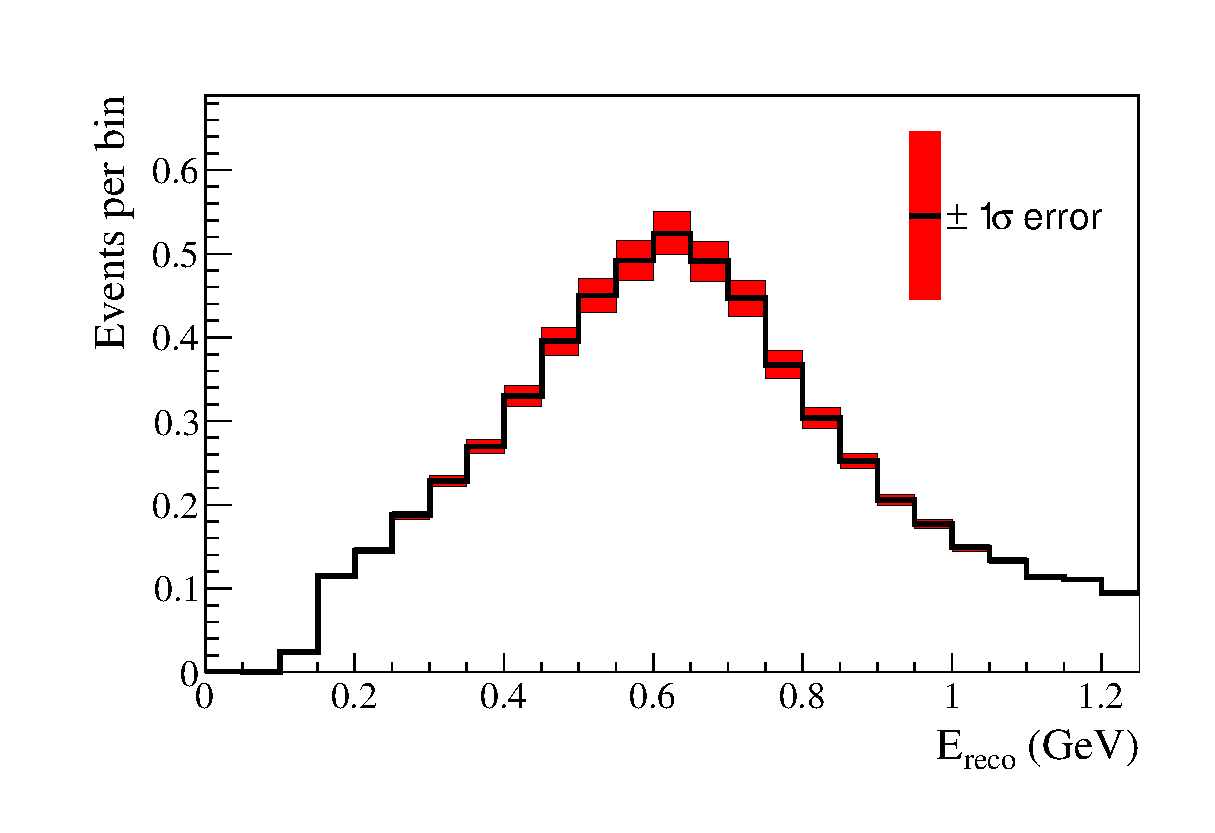
\includegraphics[width=0.9\textwidth]{joint_plots/systematics/Run17c/Asimov_A_RHC1Reoscillated_Osc_param_envelope.eps}
\caption{Electron-like, antineutrino mode}
\end{subfigure}
\begin{subfigure}[b]{0.49\textwidth} \centering
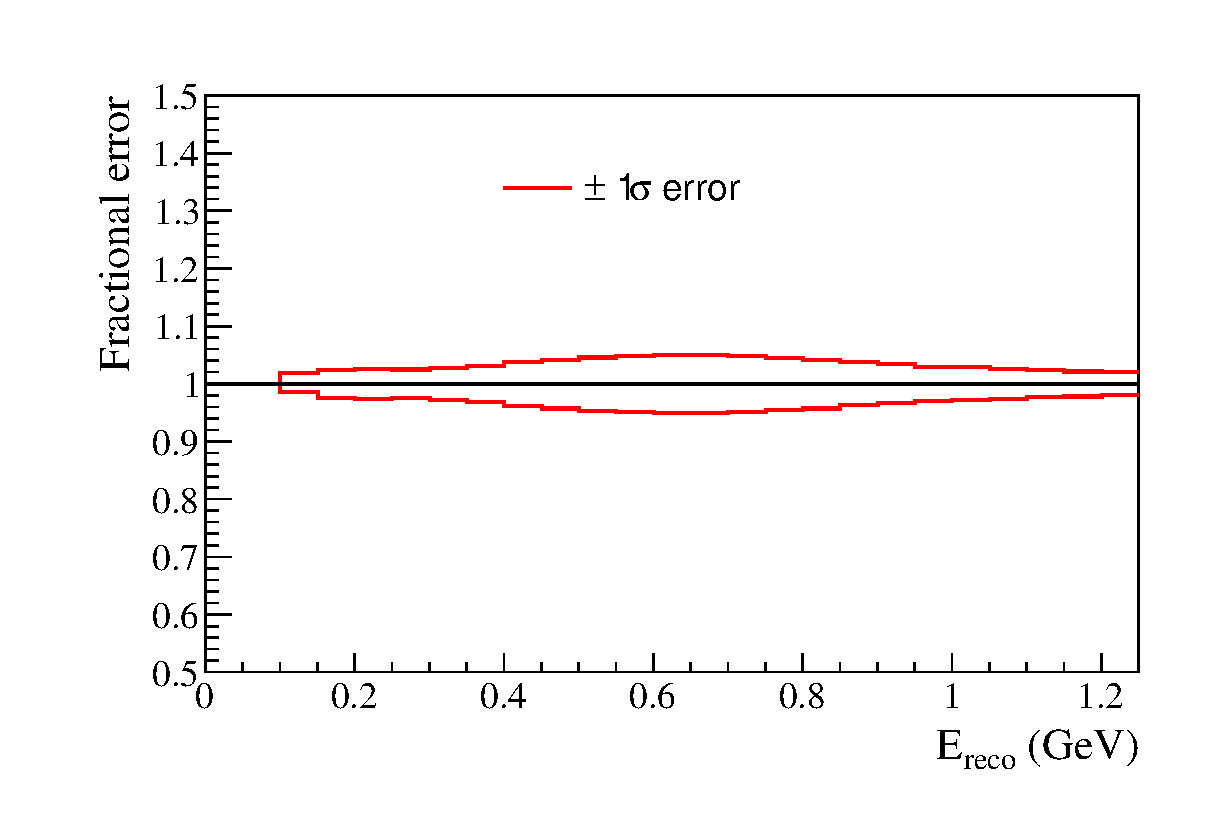
\includegraphics[width=0.9\textwidth]{joint_plots/systematics/Run17c/Asimov_A_RHC1Reoscillated_Osc_param_envelope_ratio.eps} 
\caption{Electron-like, antineutrino mode}
\end{subfigure}
%fhc ccpi-like
\begin{subfigure}[b]{0.49\textwidth} \centering
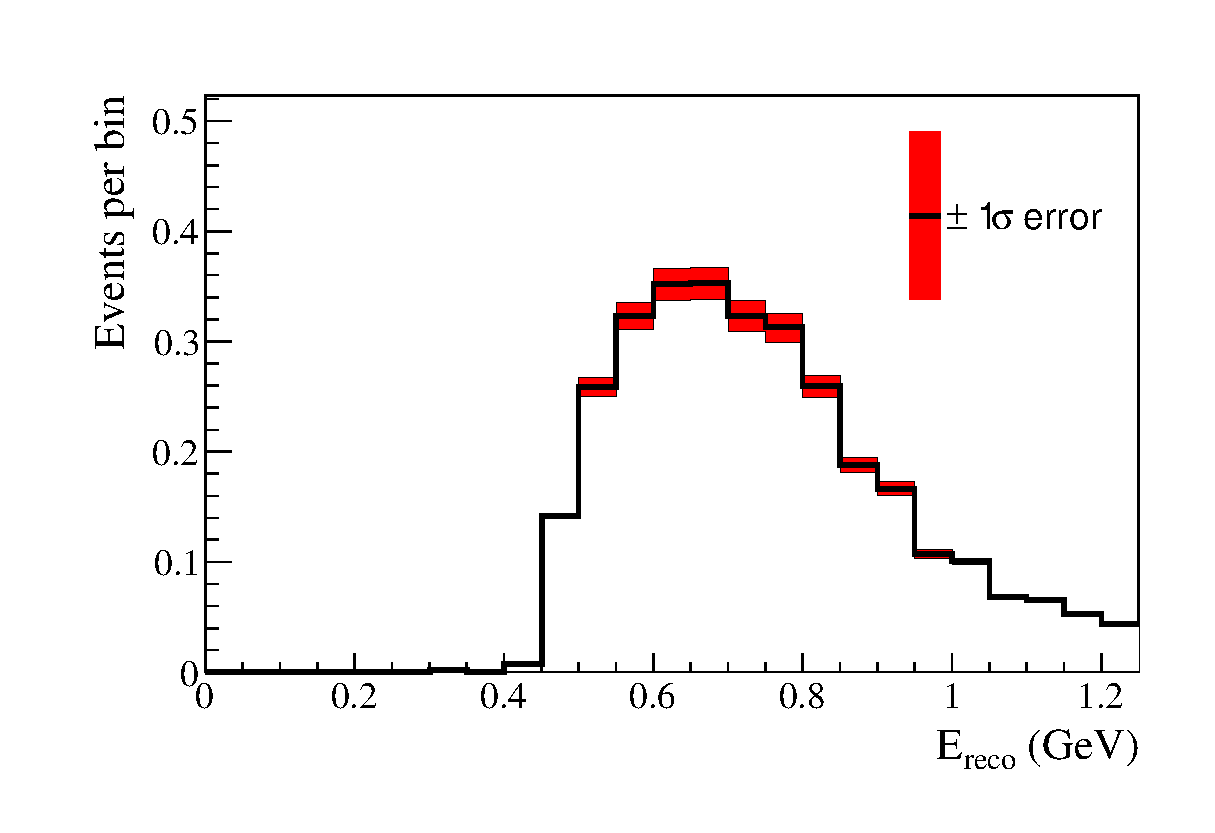
\includegraphics[width=0.9\textwidth]{joint_plots/systematics/Run17c/Asimov_A_MultiReoscillated_Osc_param_envelope.eps} 
\caption{\nueCConepi{}, neutrino mode}
\end{subfigure}
\begin{subfigure}[b]{0.49\textwidth} \centering
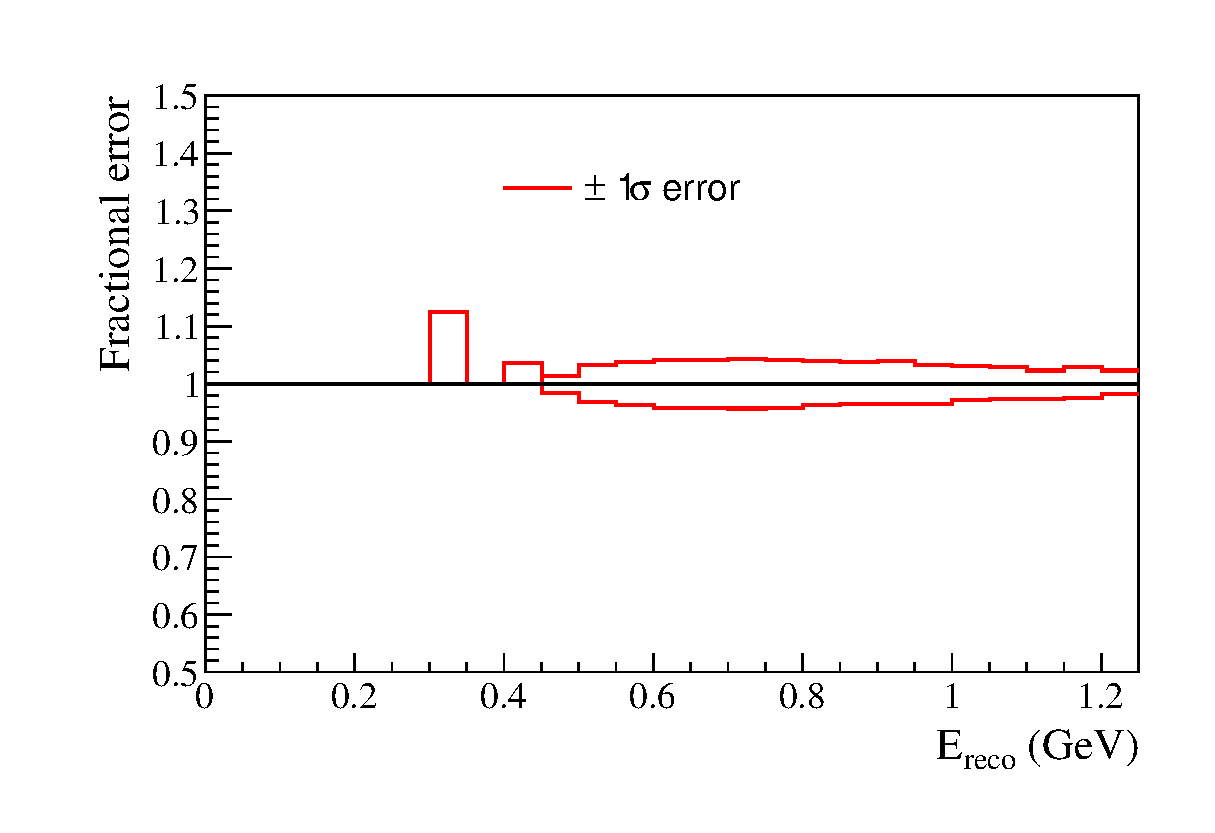
\includegraphics[width=0.9\textwidth]{joint_plots/systematics/Run17c/Asimov_A_MultiReoscillated_Osc_param_envelope_ratio.eps}
\caption{\nueCConepi{}, neutrino mode}
\end{subfigure}
\caption {
Error envelopes (left) and fractional errors (right) for the reconstructed neutrino energy spectrum
as a result of the oscillation systematic parameters.
10k toy MC experiments are generated for the Asimov data set A shown in \cref{tab:osc_params_joint_asimov}
with randomised systematic parameters, taking into account their correlations.
Since the parameters $\delta_{CP}$, $\theta_{23}$ and $\Delta m^2_{32}$ ($\Delta m^2_{13}$) and mass hierarchy
will be measured,
only the uncertainty on 
$\sin^2 \theta_{13}$,
$\sin^2 \theta_{12}$
and 
$\Delta m^2_{21}$ 
are taken into account.
BANFF tuned MC templates are used. 
The distributions correspond to the collected statistics in the full Run 1-7c data set.
The changes due to the Run 1-7c flux and covariance matrix updates are applied.
}
\label{fig:Osc_envelope_Asimov_A_run17c_elike}
\end{figure*}


\begin{figure*}[htb]
\center
%fhc mu-like
\begin{subfigure}[b]{0.49\textwidth} \centering
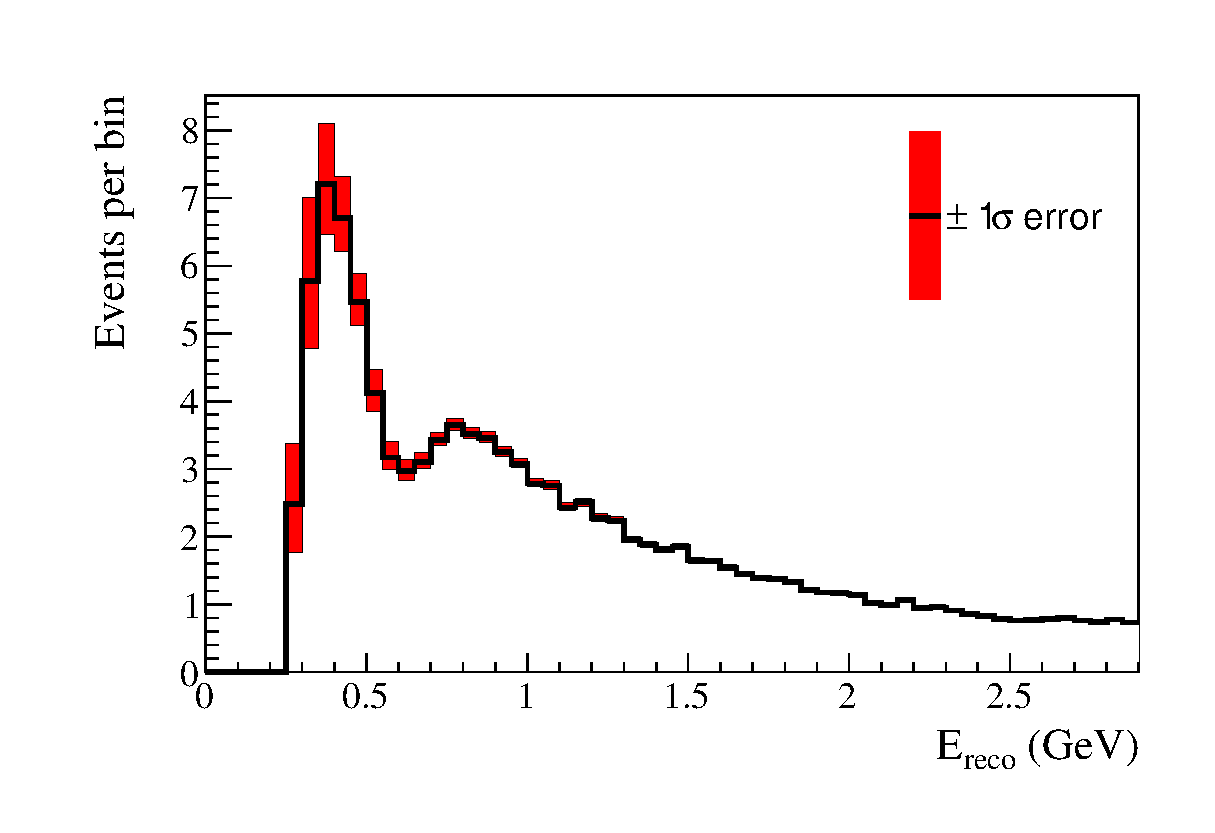
\includegraphics[width=0.9\textwidth]{joint_plots/systematics/Run17c/Asimov_A_1Rmuoscillated_SKDet_FSI_envelope.eps} 
\caption{Muon-like, neutrino mode}
\end{subfigure}
\begin{subfigure}[b]{0.49\textwidth} \centering
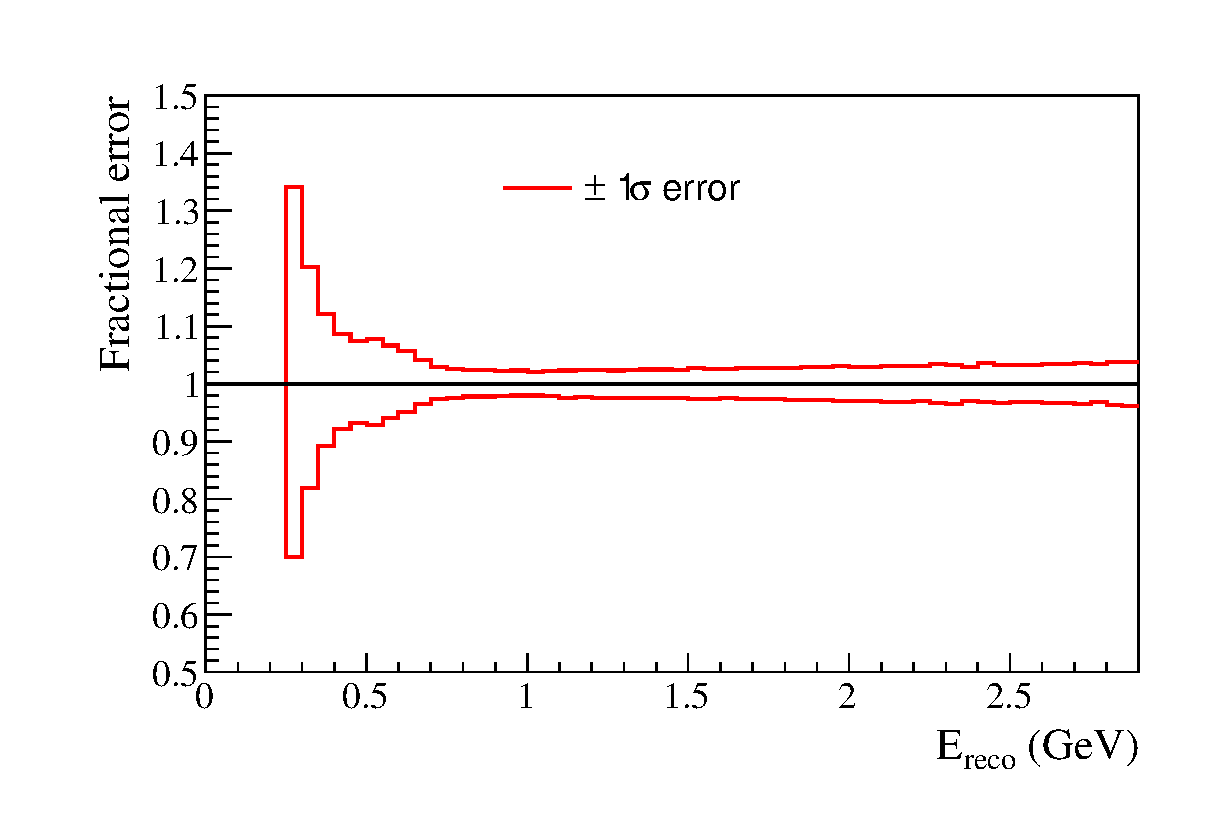
\includegraphics[width=0.9\textwidth]{joint_plots/systematics/Run17c/Asimov_A_1Rmuoscillated_SKDet_FSI_envelope_ratio.eps} 
\caption{Muon-like, neutrino mode}
\end{subfigure}
%rhc mu-like
\begin{subfigure}[b]{0.49\textwidth} \centering
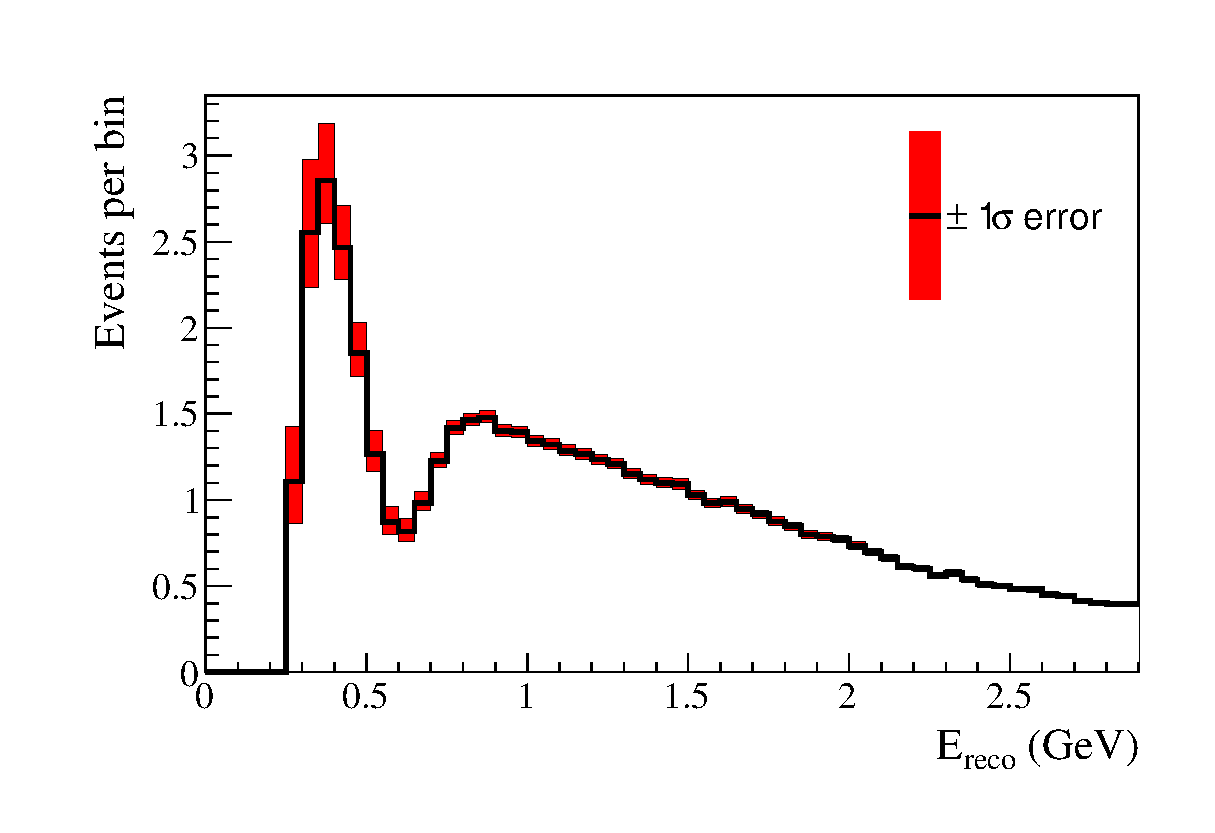
\includegraphics[width=0.9\textwidth]{joint_plots/systematics/Run17c/Asimov_A_RHC1Rmuoscillated_SKDet_FSI_envelope.eps} \\ 
\caption{Muon-like, antineutrino mode}
\end{subfigure}
\begin{subfigure}[b]{0.49\textwidth} \centering
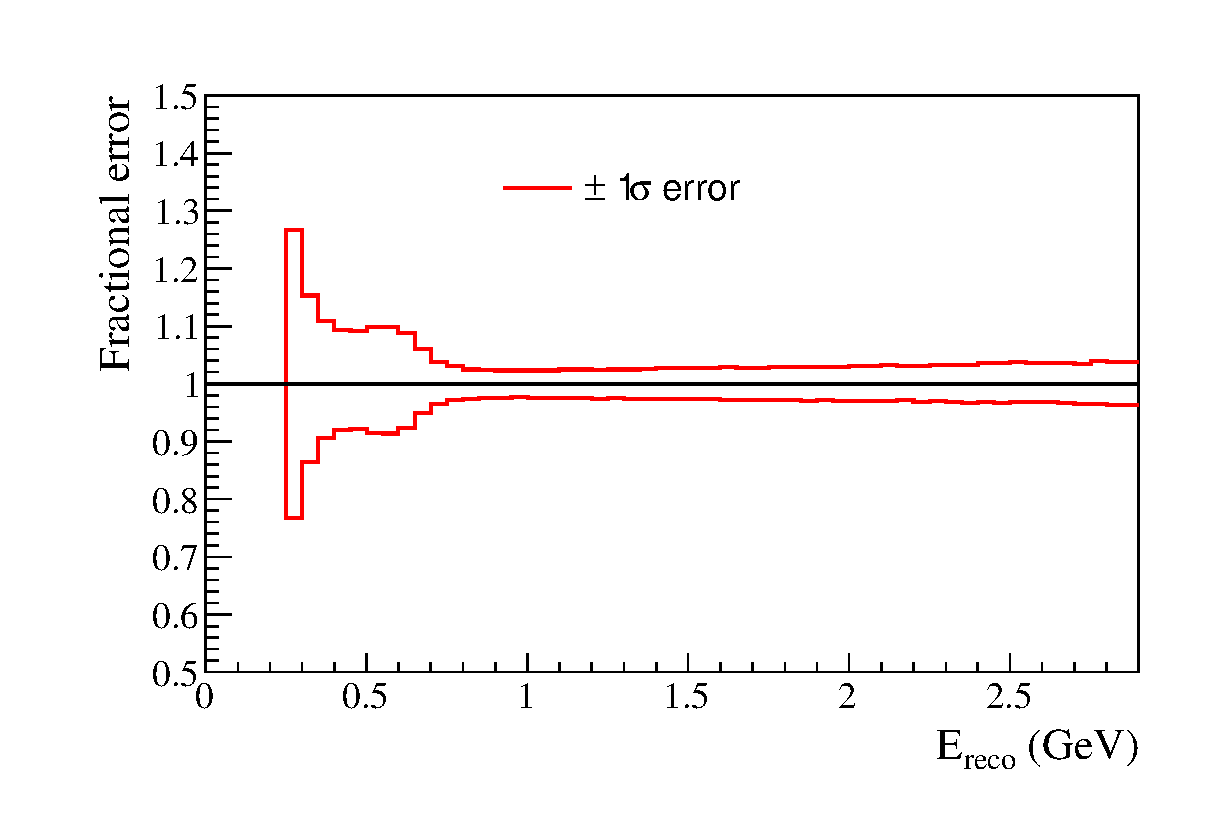
\includegraphics[width=0.9\textwidth]{joint_plots/systematics/Run17c/Asimov_A_RHC1Rmuoscillated_SKDet_FSI_envelope_ratio.eps} \\ 
\caption{Muon-like, antineutrino mode}
\end{subfigure}
%fhc e-like
\caption {
Error envelopes (left) and fractional errors (right) for the reconstructed neutrino energy spectrum
as a result of the Super-K + FSI + SI + PN systematic parameters.
	10k toy MC experiments are generated for the Asimov data set A shown in \cref{tab:osc_params_joint_asimov}
	with random systematic parameters, taking into account their correlations.
	Since the parameters $\delta_{CP}$, $\theta_{23}$ and $\Delta m^2_{32}$ ($\Delta m^2_{13}$) and mass hierarchy
will be measured,
only the uncertainty on 
$\sin^2 \theta_{13}$,
$\sin^2 \theta_{12}$
and 
$\Delta m^2_{21}$ 
are taken into account.
BANFF tuned MC templates are used. 
The distributions correspond to the collected statistics in the full Run 1-7c data set.
The changes due to the Run 1-7c flux and covariance matrix updates are applied.
}
\label{fig:SKDet_FSI_envelope_Asimov_A_run17c_mulike}
\end{figure*}


\begin{figure*}[htb]
\center

\begin{subfigure}[b]{0.49\textwidth} \centering
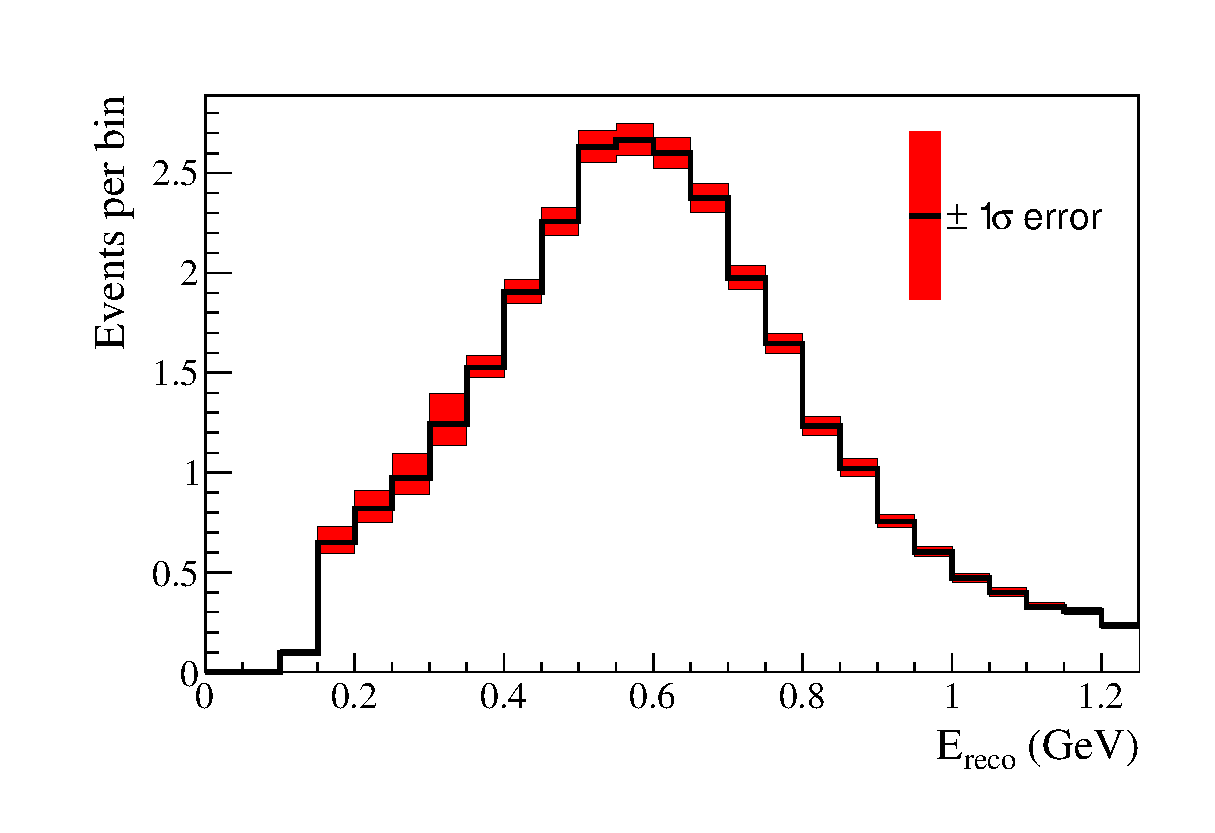
\includegraphics[width=0.9\textwidth]{joint_plots/systematics/Run17c/Asimov_A_1Reoscillated_SKDet_FSI_envelope.eps} 
\caption{Electron-like, neutrino mode}
\end{subfigure}
\begin{subfigure}[b]{0.49\textwidth} \centering
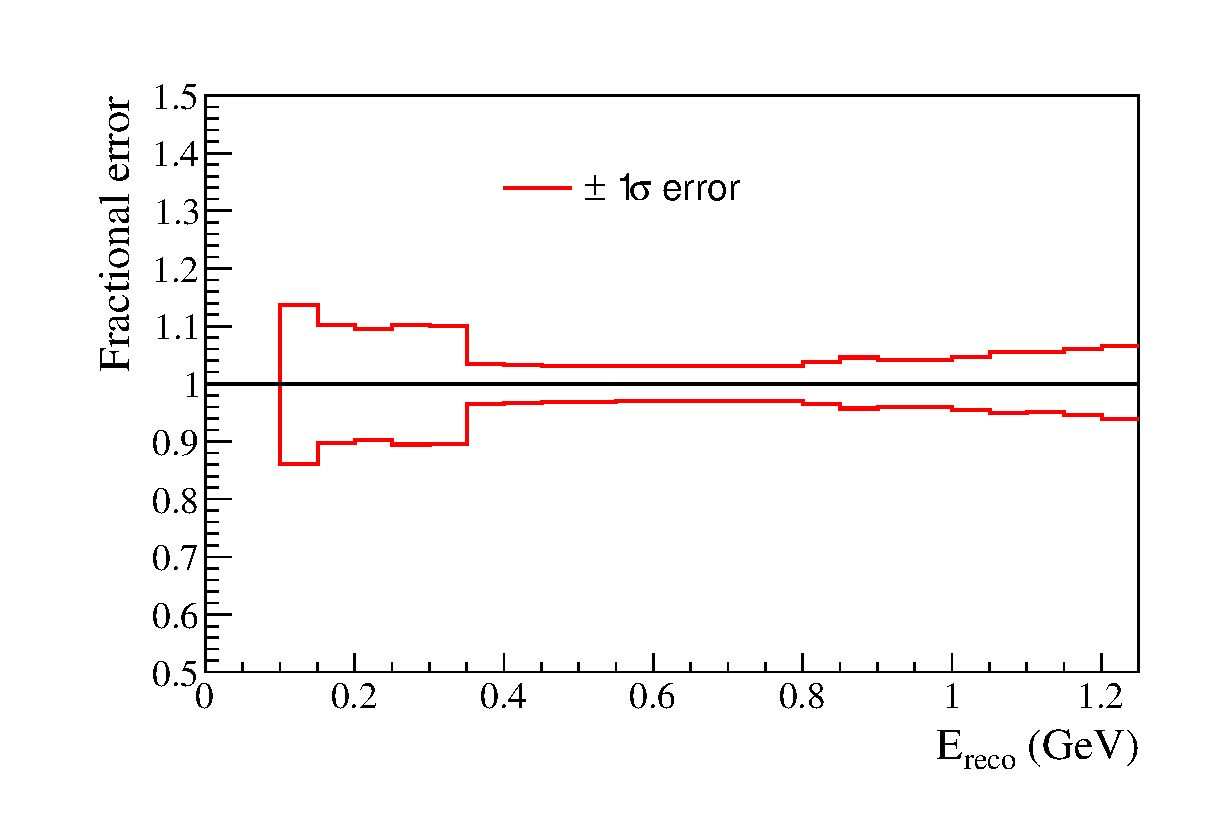
\includegraphics[width=0.9\textwidth]{joint_plots/systematics/Run17c/Asimov_A_1Reoscillated_SKDet_FSI_envelope_ratio.eps} 
\caption{Electron-like, neutrino mode}
\end{subfigure}
%rhc e-like
\begin{subfigure}[b]{0.49\textwidth} \centering
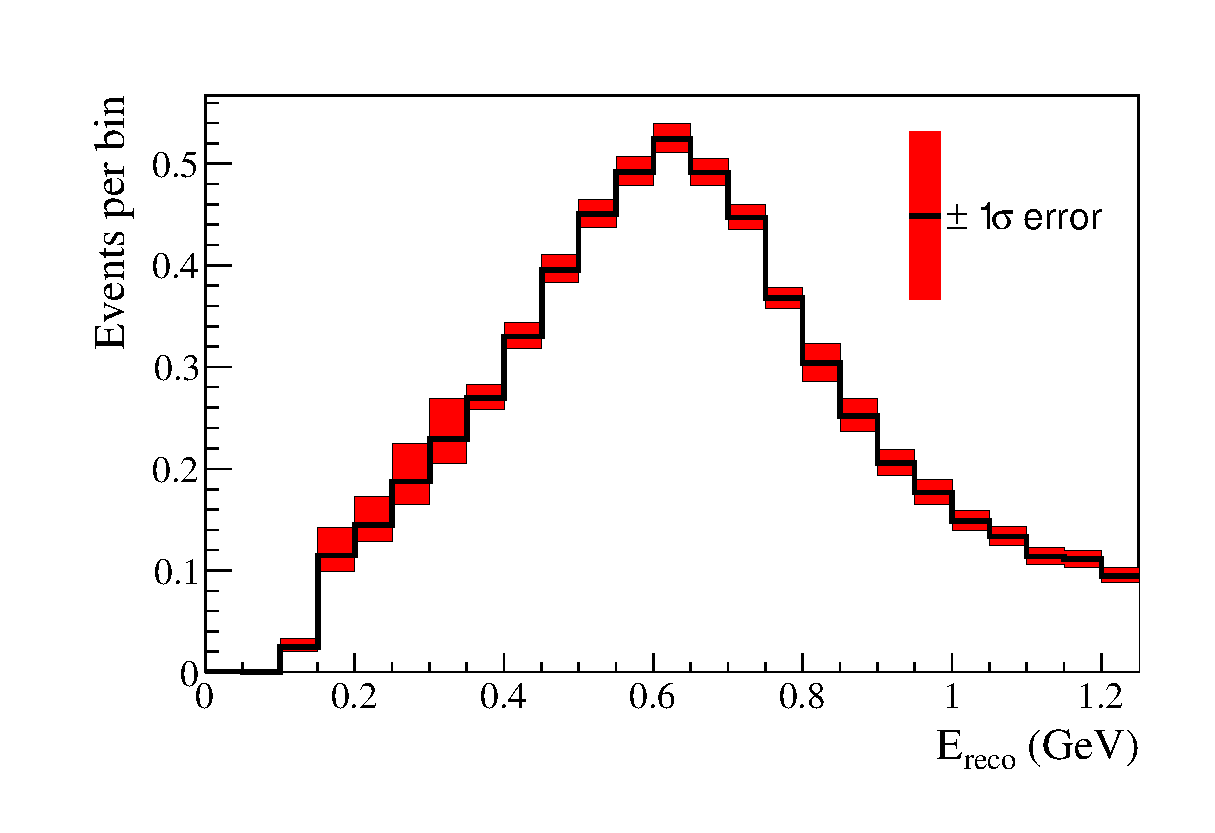
\includegraphics[width=0.9\textwidth]{joint_plots/systematics/Run17c/Asimov_A_RHC1Reoscillated_SKDet_FSI_envelope.eps} 
\caption{Electron-like, antineutrino mode}
\end{subfigure}
\begin{subfigure}[b]{0.49\textwidth} \centering
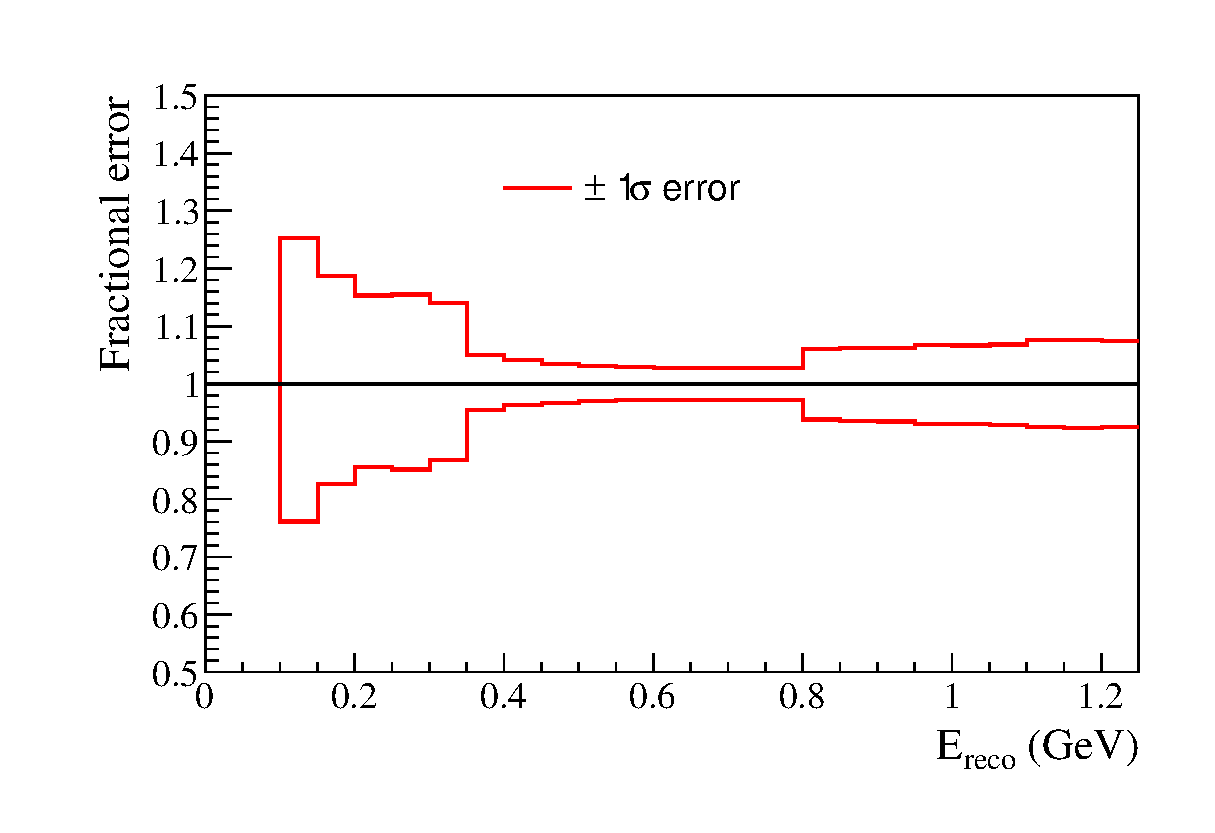
\includegraphics[width=0.9\textwidth]{joint_plots/systematics/Run17c/Asimov_A_RHC1Reoscillated_SKDet_FSI_envelope_ratio.eps} 
\caption{Electron-like, antineutrino mode}
\end{subfigure}
%fhc ccpi-like
\begin{subfigure}[b]{0.49\textwidth} \centering
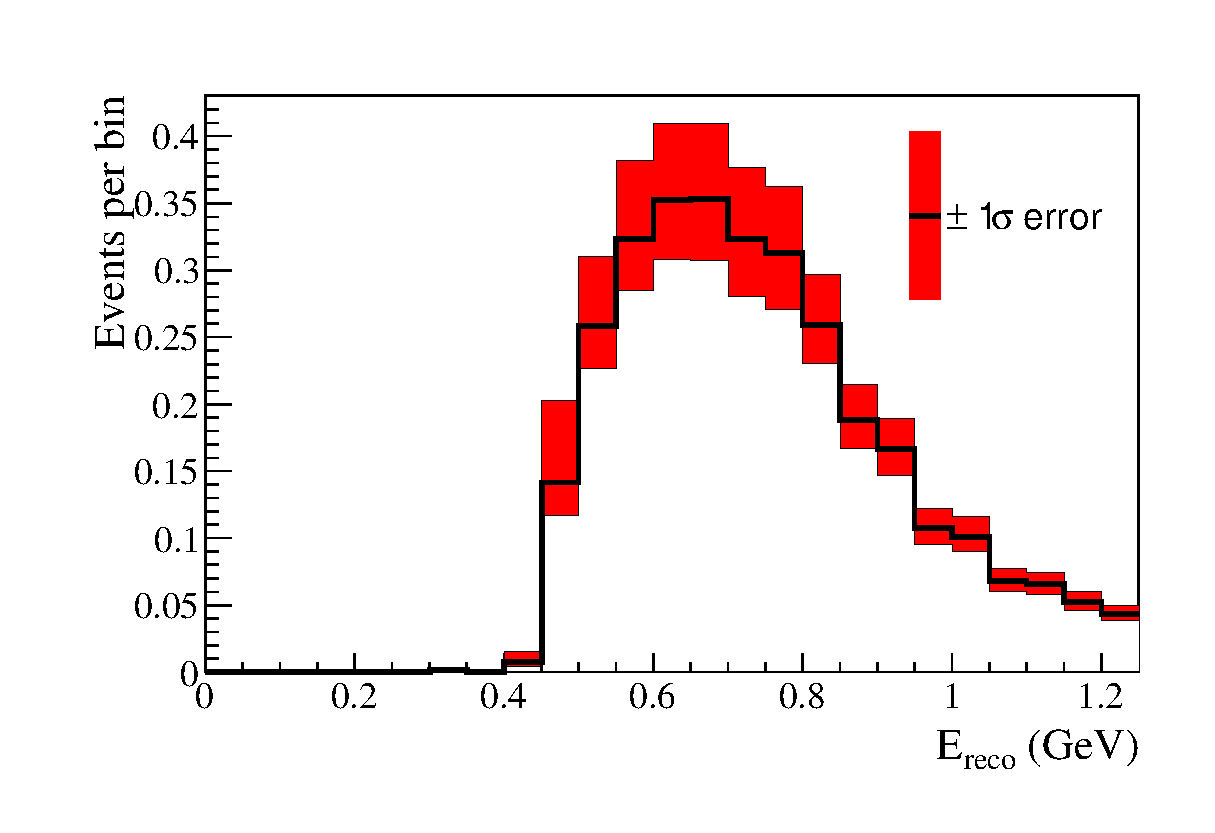
\includegraphics[width=0.9\textwidth]{joint_plots/systematics/Run17c/Asimov_A_MultiReoscillated_SKDet_FSI_envelope.eps} 
\caption{\nueCConepi{}, neutrino mode}
\end{subfigure}
\begin{subfigure}[b]{0.49\textwidth} \centering
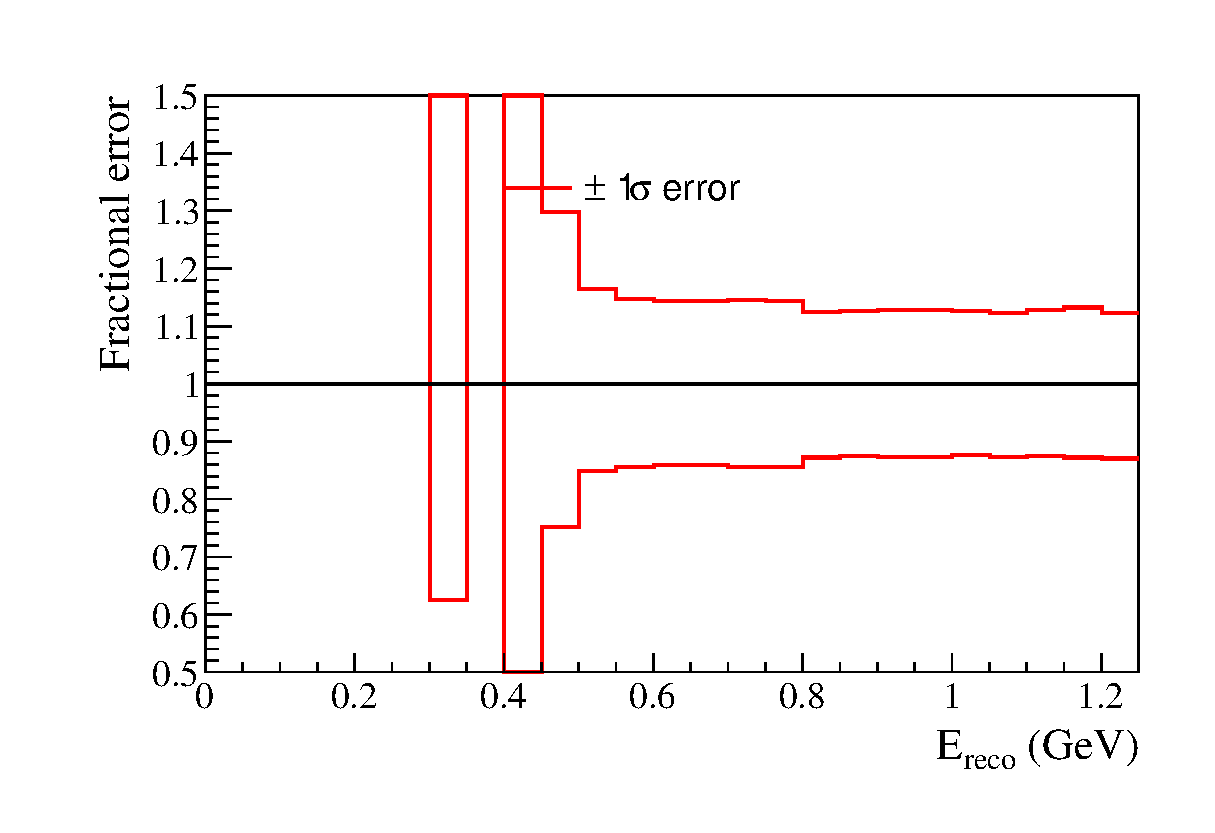
\includegraphics[width=0.9\textwidth]{joint_plots/systematics/Run17c/Asimov_A_MultiReoscillated_SKDet_FSI_envelope_ratio.eps} 
\caption{\nueCConepi{}, neutrino mode}
\end{subfigure}
\caption {
Error envelopes (left) and fractional errors (right) for the reconstructed neutrino energy spectrum
as a result of the Super-K + FSI + SI + PN systematic parameters.
10k toy MC experiments are generated for the Asimov data set A shown in \cref{tab:osc_params_joint_asimov}
with randomised systematic parameters, taking into account their correlations.
Since the parameters $\delta_{CP}$, $\theta_{23}$ and $\Delta m^2_{32}$ ($\Delta m^2_{13}$) and mass hierarchy
will be measured,
only the uncertainty on 
$\sin^2 \theta_{13}$,
$\sin^2 \theta_{12}$
and 
$\Delta m^2_{21}$ 
are taken into account.
BANFF tuned MC templates are used. 
The distributions correspond to the collected statistics in the full Run 1-7c data set.
The changes due to the Run 1-7c flux and covariance matrix updates are applied.
}
\label{fig:SKDet_FSI_envelope_Asimov_A_run17c_elike}
\end{figure*}




\begin{figure*}[htb]
\center
%fhc mu-like
\begin{subfigure}[b]{0.49\textwidth} \centering
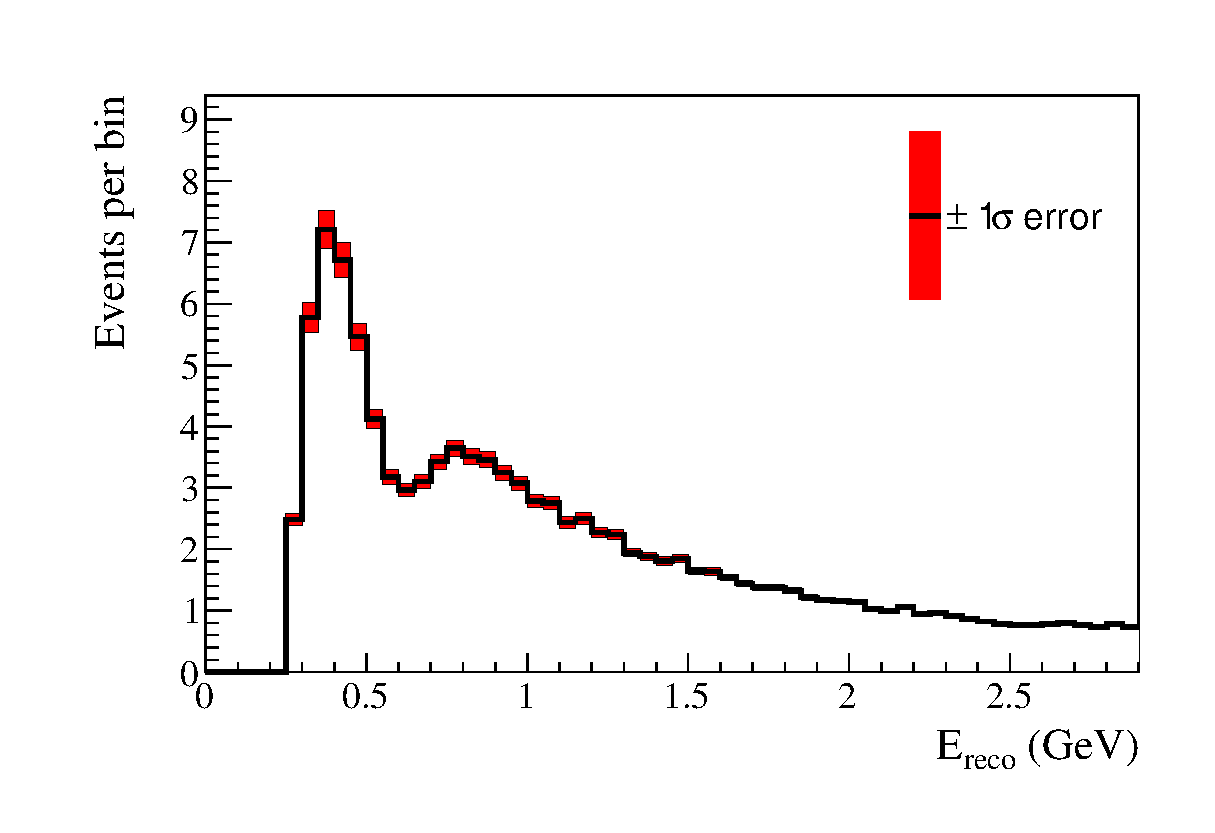
\includegraphics[width=0.9\textwidth]{joint_plots/systematics/Run17c/Asimov_A_1Rmuoscillated_BANFF_flux_envelope.eps} 
\caption{Muon-like, neutrino mode}
\end{subfigure}
\begin{subfigure}[b]{0.49\textwidth} \centering
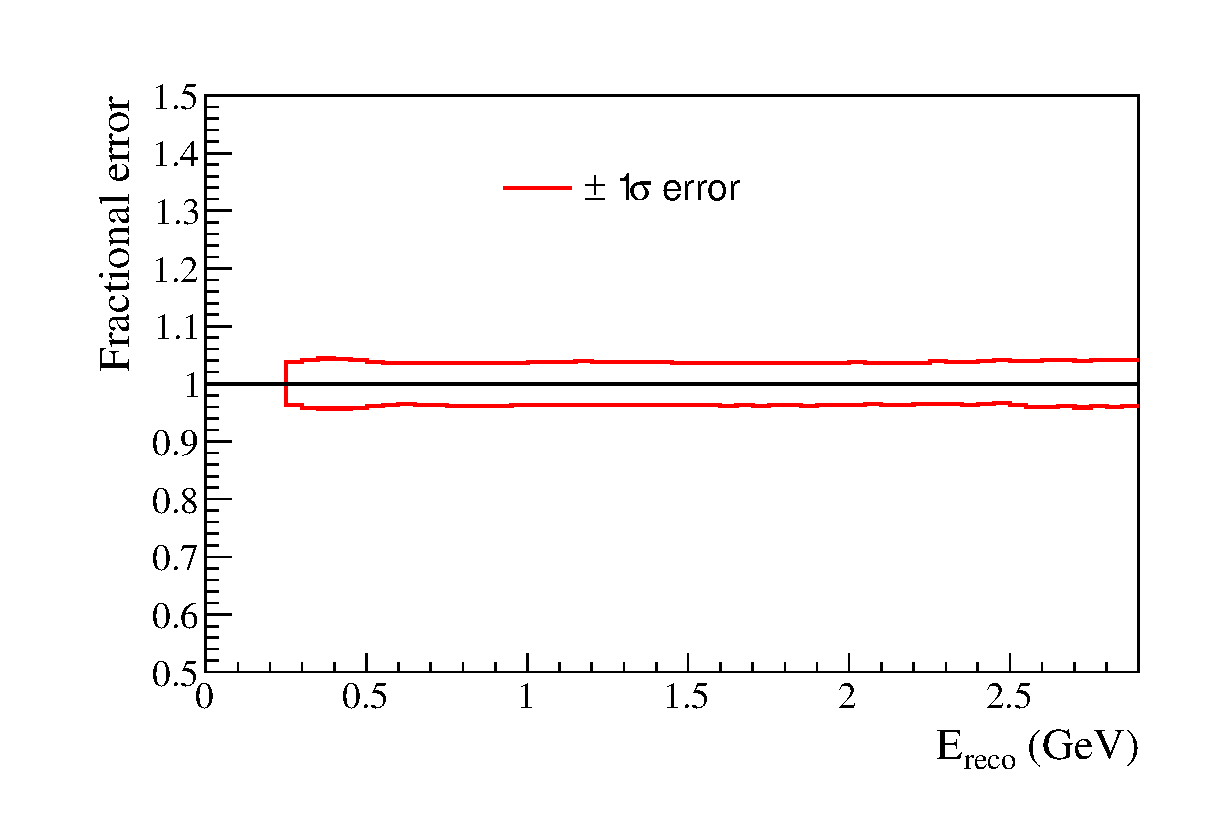
\includegraphics[width=0.9\textwidth]{joint_plots/systematics/Run17c/Asimov_A_1Rmuoscillated_BANFF_flux_envelope_ratio.eps} 
\caption{Muon-like, neutrino mode}
\end{subfigure}
%rhc mu-like
\begin{subfigure}[b]{0.49\textwidth} \centering
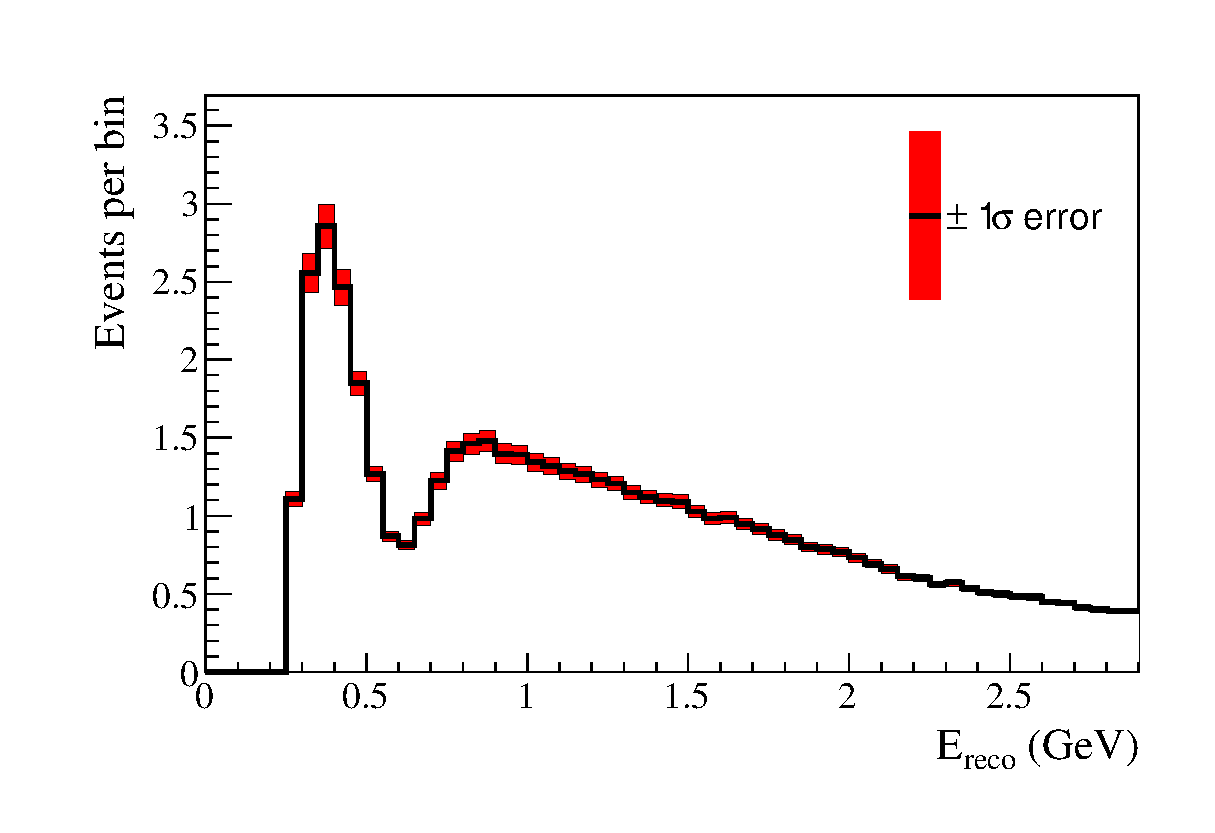
\includegraphics[width=0.9\textwidth]{joint_plots/systematics/Run17c/Asimov_A_RHC1Rmuoscillated_BANFF_flux_envelope.eps} \\ 
\caption{Muon-like, antineutrino mode}
\end{subfigure}
\begin{subfigure}[b]{0.49\textwidth} \centering
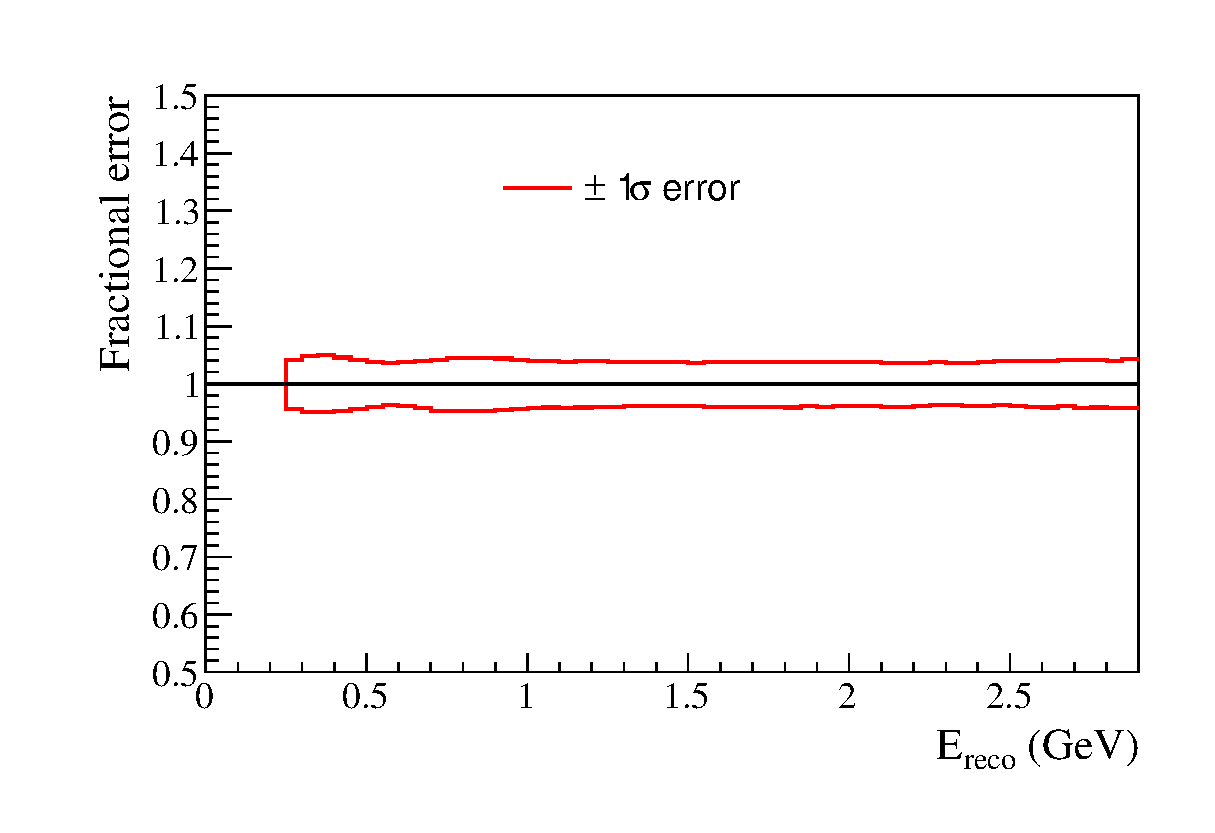
\includegraphics[width=0.9\textwidth]{joint_plots/systematics/Run17c/Asimov_A_RHC1Rmuoscillated_BANFF_flux_envelope_ratio.eps} \\ 
\caption{Muon-like, antineutrino mode}
\end{subfigure}
%fhc e-like
\caption {
Error envelopes (left) and fractional errors (right) for the reconstructed neutrino energy spectrum
as a result of the flux systematic parameters.
	10k toy MC experiments are generated for the Asimov data set A shown in \cref{tab:osc_params_joint_asimov}
	with random systematic parameters, taking into account their correlations.
	Since the parameters $\delta_{CP}$, $\theta_{23}$ and $\Delta m^2_{32}$ ($\Delta m^2_{13}$) and mass hierarchy
will be measured,
only the uncertainty on 
$\sin^2 \theta_{13}$,
$\sin^2 \theta_{12}$
and 
$\Delta m^2_{21}$ 
are taken into account.
BANFF tuned MC templates are used. 
The distributions correspond to the collected statistics in the full Run 1-7c data set.
The changes due to the Run 1-7c flux and covariance matrix updates are applied.
}
\label{fig:flux_envelope_Asimov_A_run17c_mulike}
\end{figure*}


\begin{figure*}[htb]
\center

\begin{subfigure}[b]{0.49\textwidth} \centering
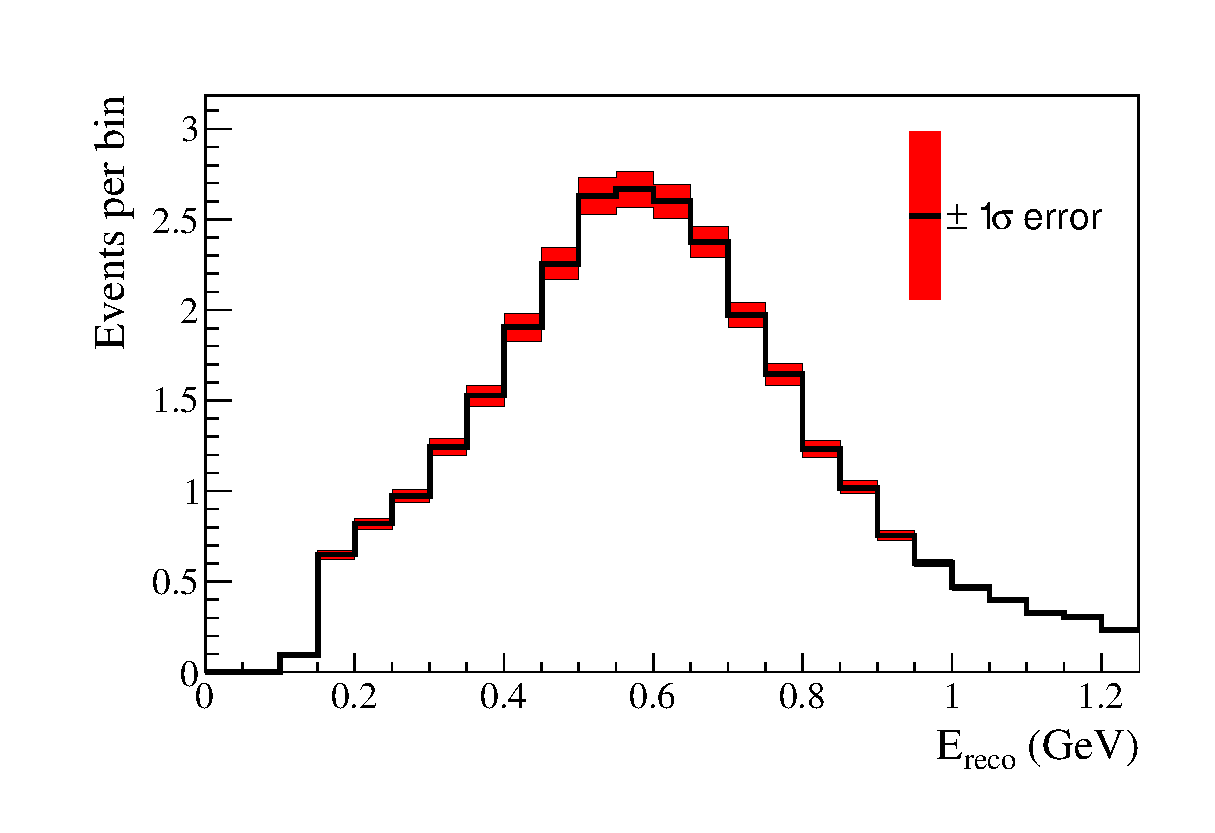
\includegraphics[width=0.9\textwidth]{joint_plots/systematics/Run17c/Asimov_A_1Reoscillated_BANFF_flux_envelope.eps} 
\caption{Electron-like, neutrino mode}
\end{subfigure}
\begin{subfigure}[b]{0.49\textwidth} \centering
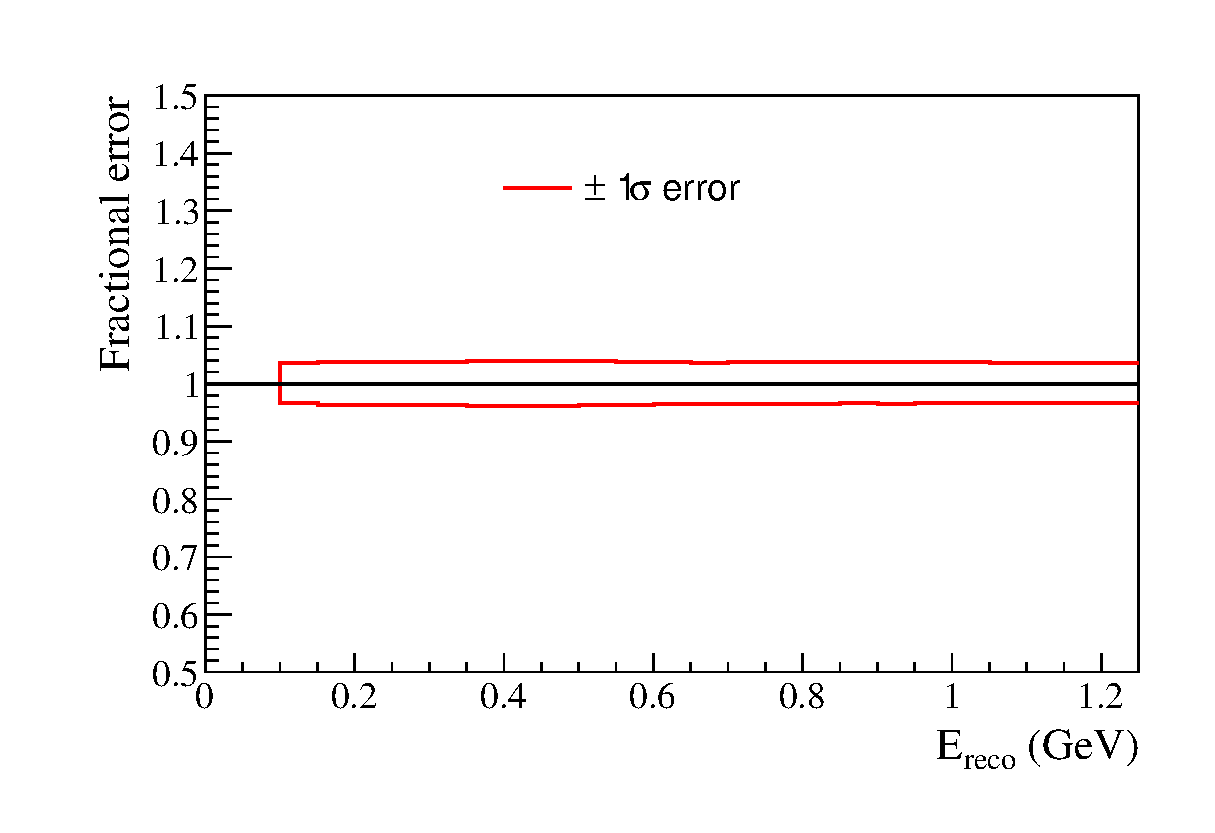
\includegraphics[width=0.9\textwidth]{joint_plots/systematics/Run17c/Asimov_A_1Reoscillated_BANFF_flux_envelope_ratio.eps} 
\caption{Electron-like, neutrino mode}
\end{subfigure}
%rhc e-like
\begin{subfigure}[b]{0.49\textwidth} \centering
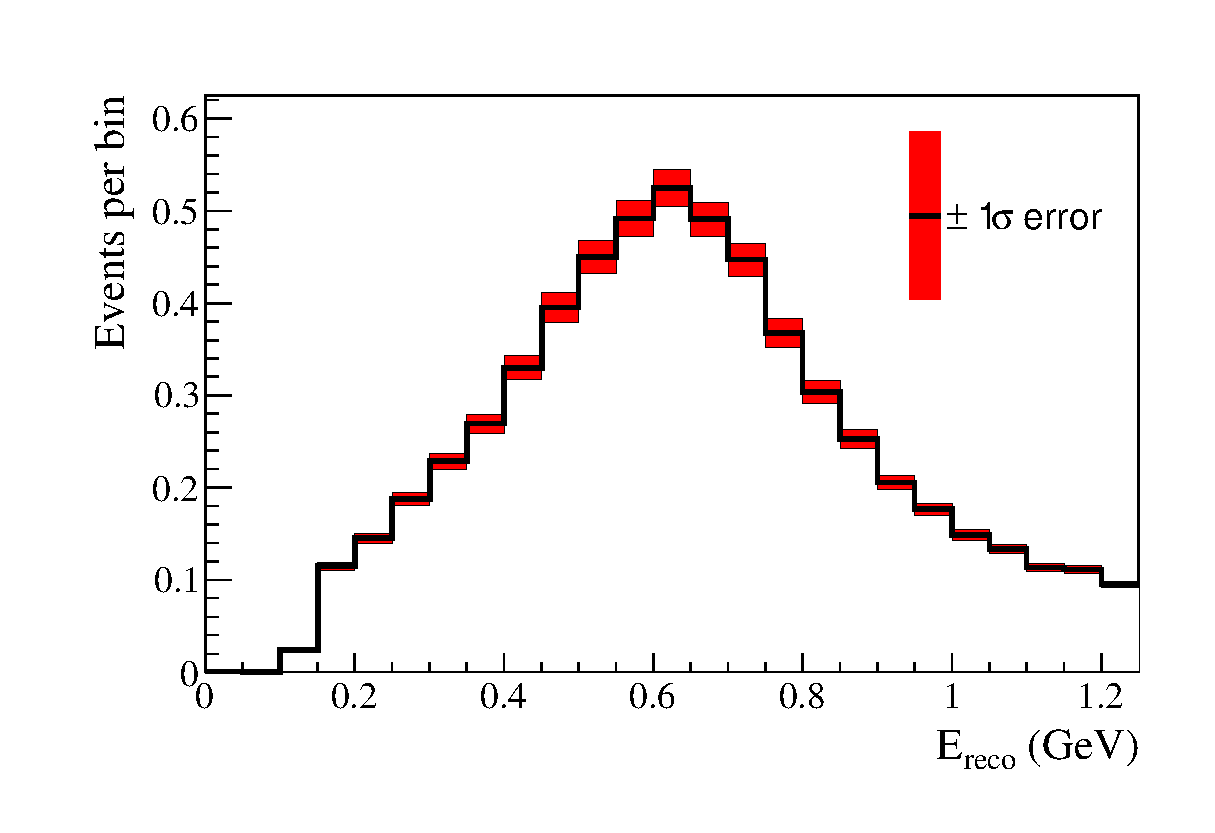
\includegraphics[width=0.9\textwidth]{joint_plots/systematics/Run17c/Asimov_A_RHC1Reoscillated_BANFF_flux_envelope.eps} 
\caption{Electron-like, antineutrino mode}
\end{subfigure}
\begin{subfigure}[b]{0.49\textwidth} \centering
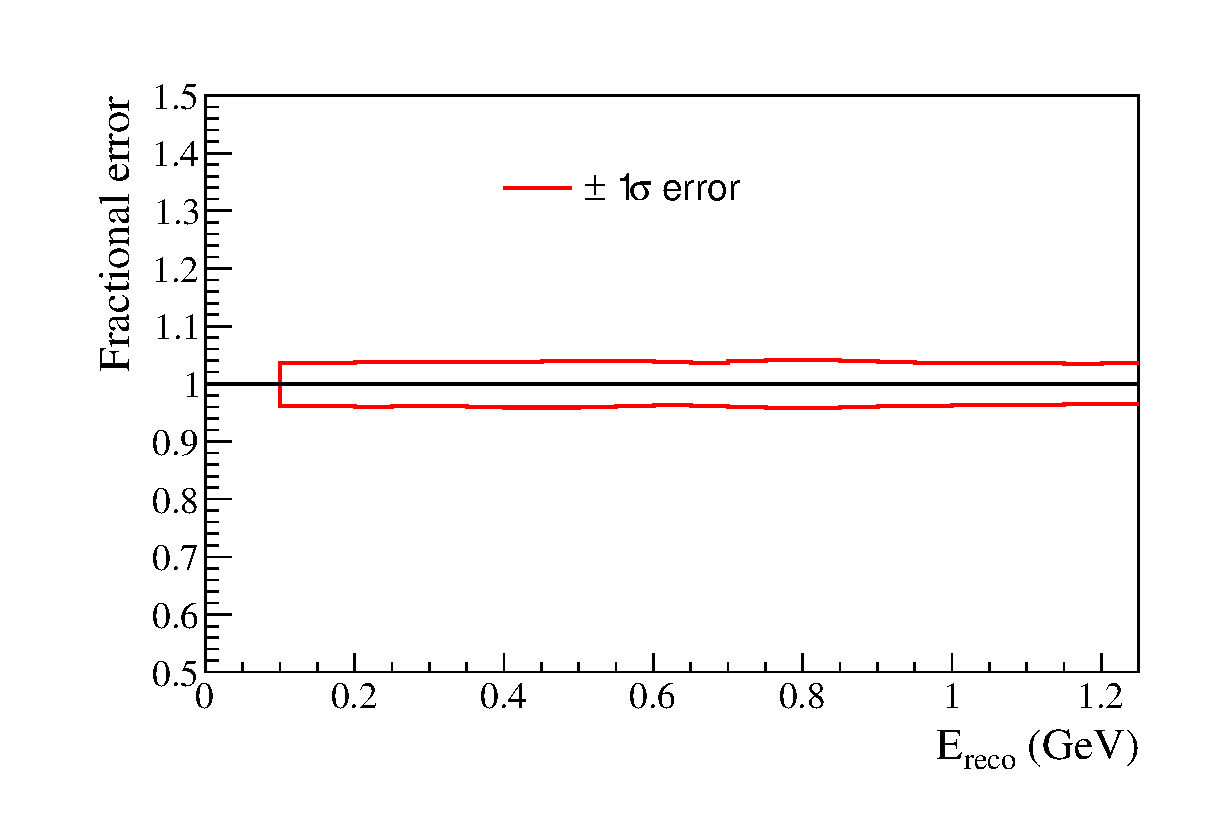
\includegraphics[width=0.9\textwidth]{joint_plots/systematics/Run17c/Asimov_A_RHC1Reoscillated_BANFF_flux_envelope_ratio.eps} 
\caption{Electron-like, antineutrino mode}
\end{subfigure}
%fhc ccpi-like
\begin{subfigure}[b]{0.49\textwidth} \centering
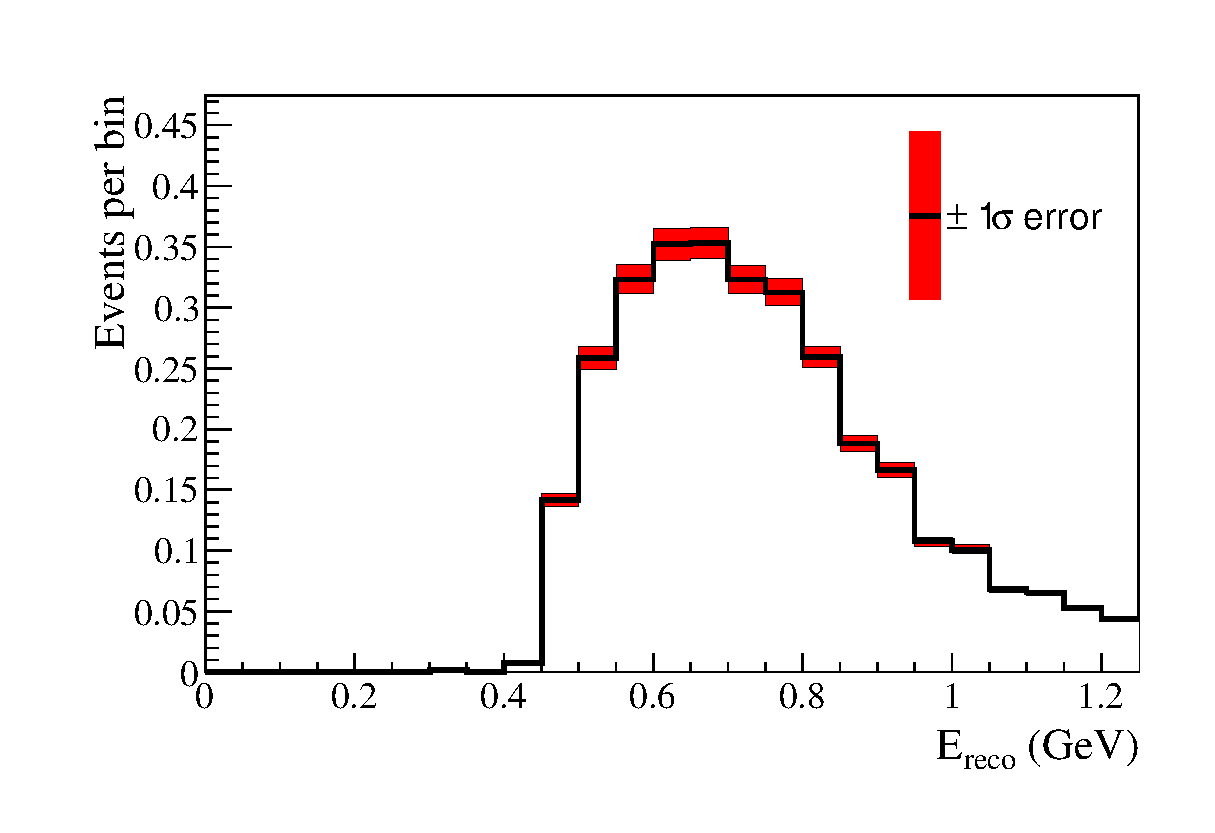
\includegraphics[width=0.9\textwidth]{joint_plots/systematics/Run17c/Asimov_A_MultiReoscillated_BANFF_flux_envelope.eps} 
\caption{\nueCConepi{}, neutrino mode}
\end{subfigure}
\begin{subfigure}[b]{0.49\textwidth} \centering
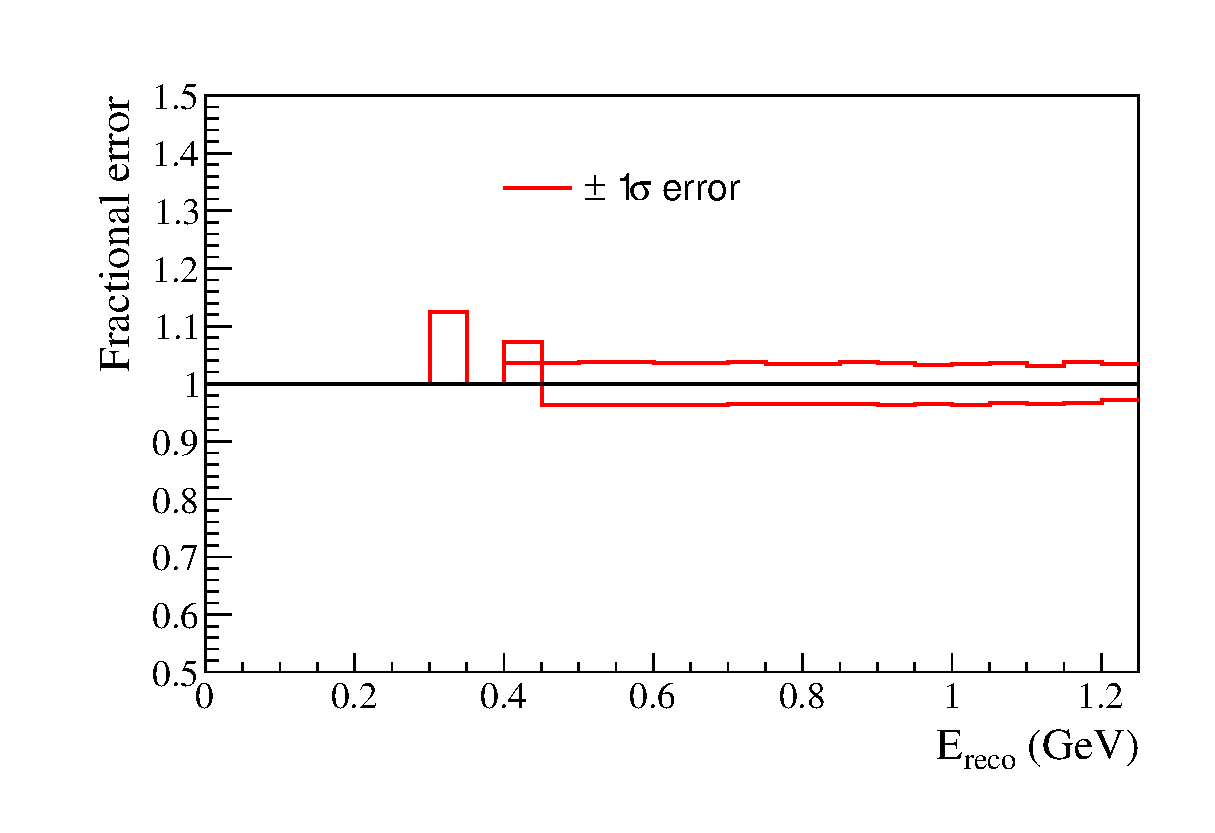
\includegraphics[width=0.9\textwidth]{joint_plots/systematics/Run17c/Asimov_A_MultiReoscillated_BANFF_flux_envelope_ratio.eps} 
\caption{\nueCConepi{}, neutrino mode}
\end{subfigure}
\caption {
Error envelopes (left) and fractional errors (right) for the reconstructed neutrino energy spectrum
as a result of the flux systematic parameters.
10k toy MC experiments are generated for the Asimov data set A shown in \cref{tab:osc_params_joint_asimov}
with randomised systematic parameters, taking into account their correlations.
Since the parameters $\delta_{CP}$, $\theta_{23}$ and $\Delta m^2_{32}$ ($\Delta m^2_{13}$) and mass hierarchy
will be measured,
only the uncertainty on 
$\sin^2 \theta_{13}$,
$\sin^2 \theta_{12}$
and 
$\Delta m^2_{21}$ 
are taken into account.
BANFF tuned MC templates are used. 
The distributions correspond to the collected statistics in the full Run 1-7c data set.
The changes due to the Run 1-7c flux and covariance matrix updates are applied.
}
\label{fig:flux_envelope_Asimov_A_run17c_elike}
\end{figure*}


\begin{figure*}[htb]
\center
%fhc mu-like
\begin{subfigure}[b]{0.49\textwidth} \centering
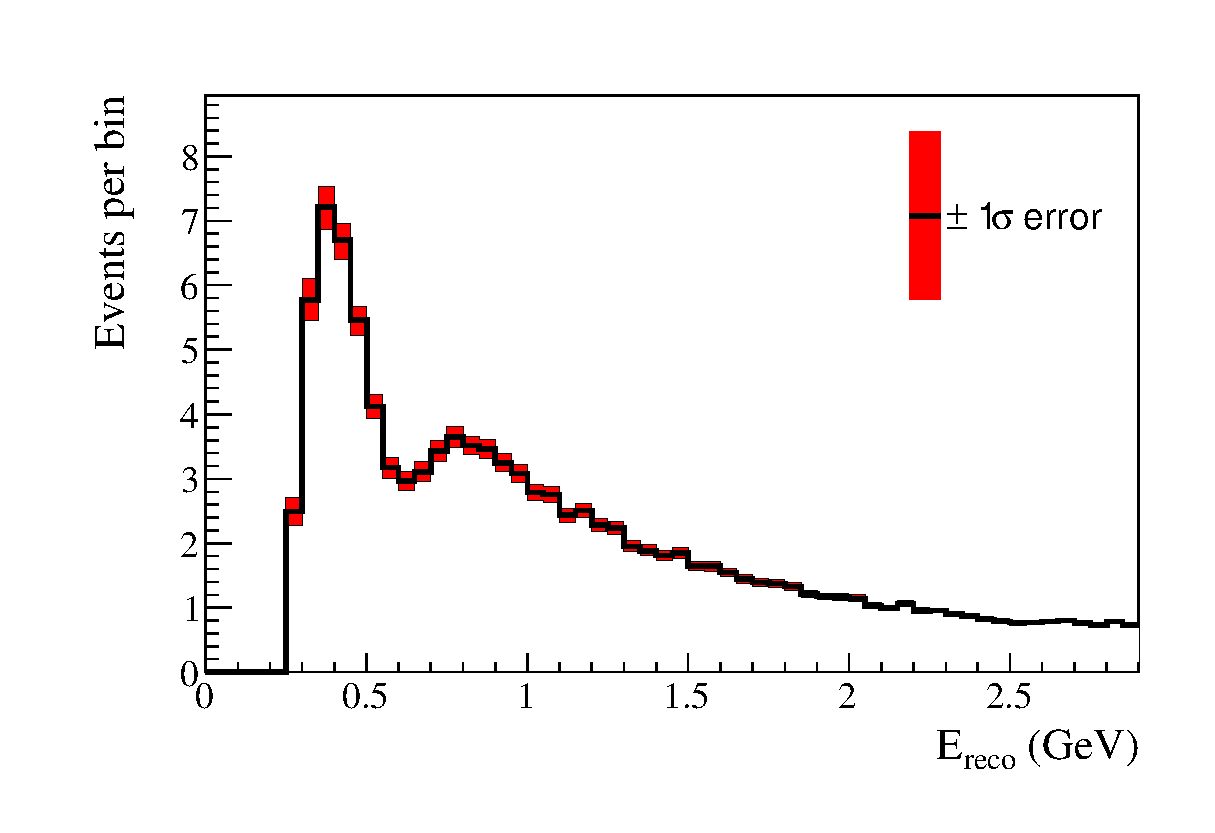
\includegraphics[width=0.9\textwidth]{joint_plots/systematics/Run17c/Asimov_A_1Rmuoscillated_BANFF_xsec_envelope.eps} 
\caption{Muon-like, neutrino mode}
\end{subfigure}
\begin{subfigure}[b]{0.49\textwidth} \centering
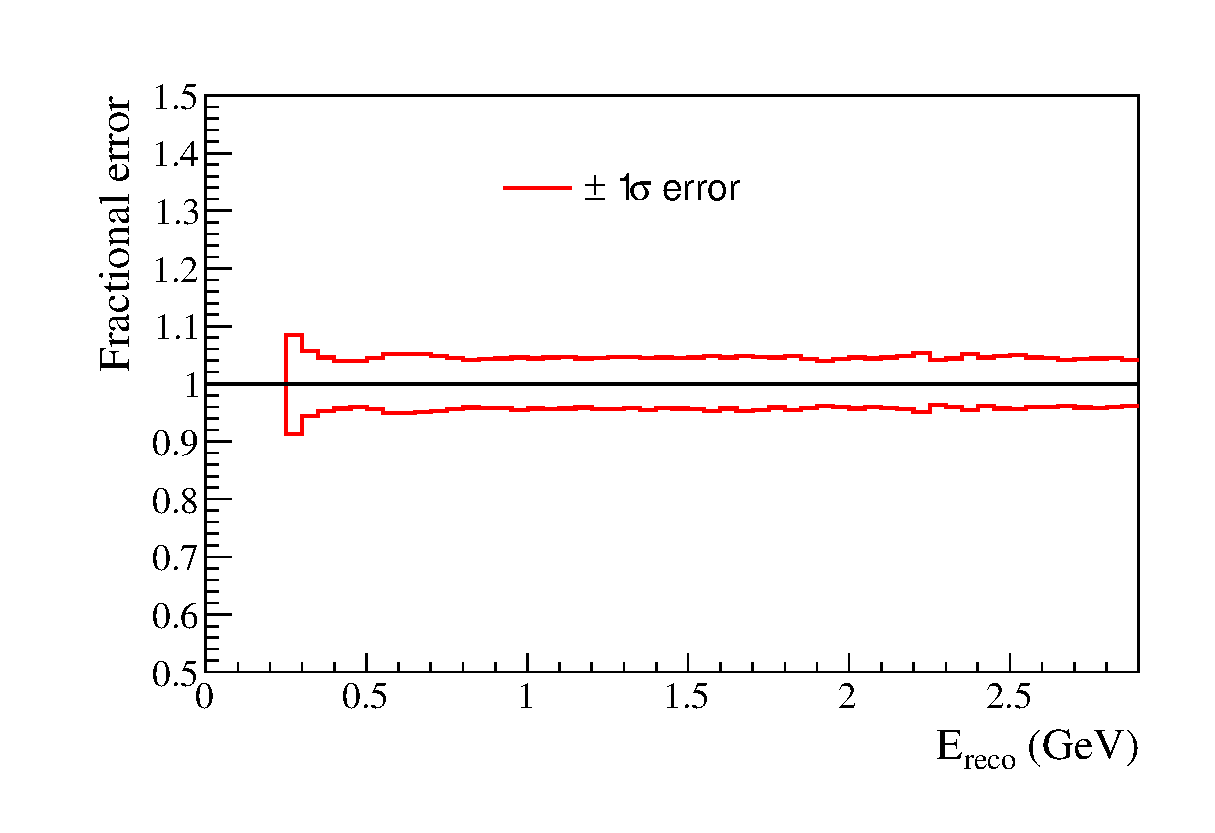
\includegraphics[width=0.9\textwidth]{joint_plots/systematics/Run17c/Asimov_A_1Rmuoscillated_BANFF_xsec_envelope_ratio.eps} 
\caption{Muon-like, neutrino mode}
\end{subfigure}
%rhc mu-like
\begin{subfigure}[b]{0.49\textwidth} \centering
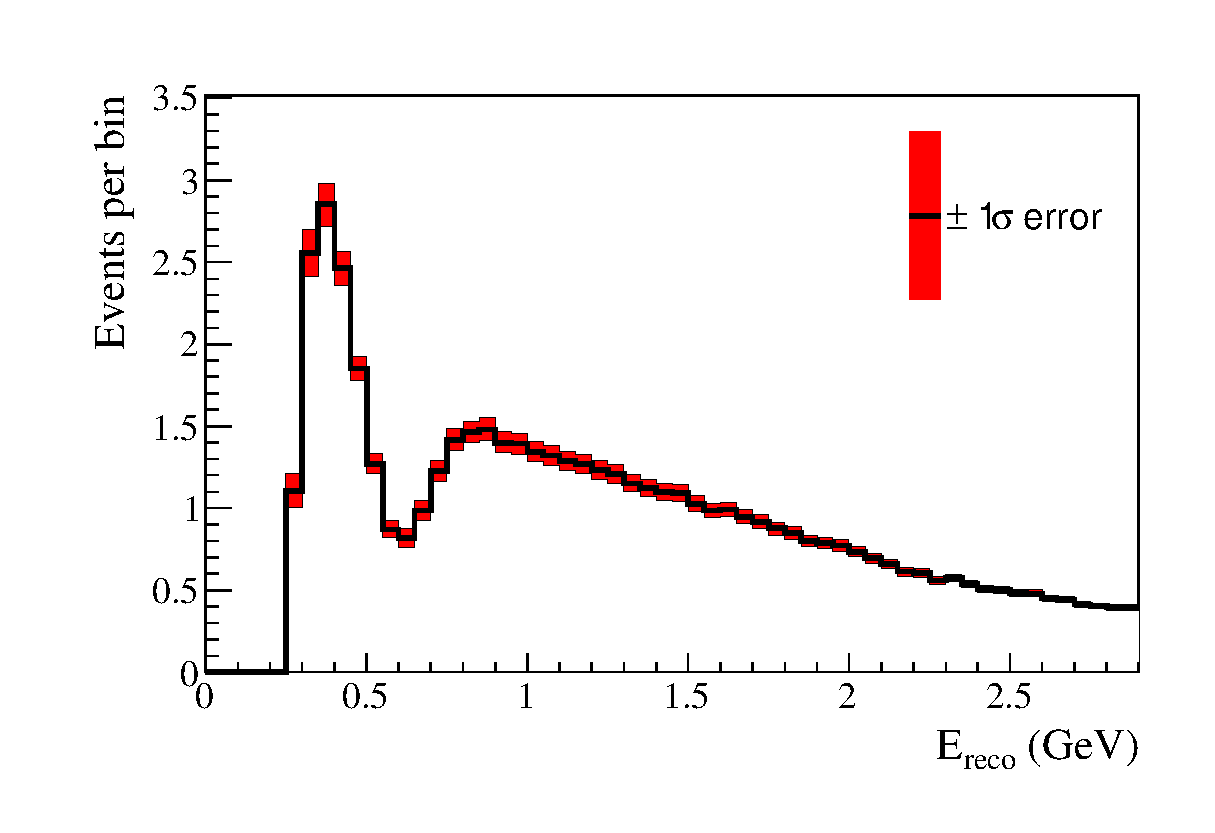
\includegraphics[width=0.9\textwidth]{joint_plots/systematics/Run17c/Asimov_A_RHC1Rmuoscillated_BANFF_xsec_envelope.eps} \\ 
\caption{Muon-like, antineutrino mode}
\end{subfigure}
\begin{subfigure}[b]{0.49\textwidth} \centering
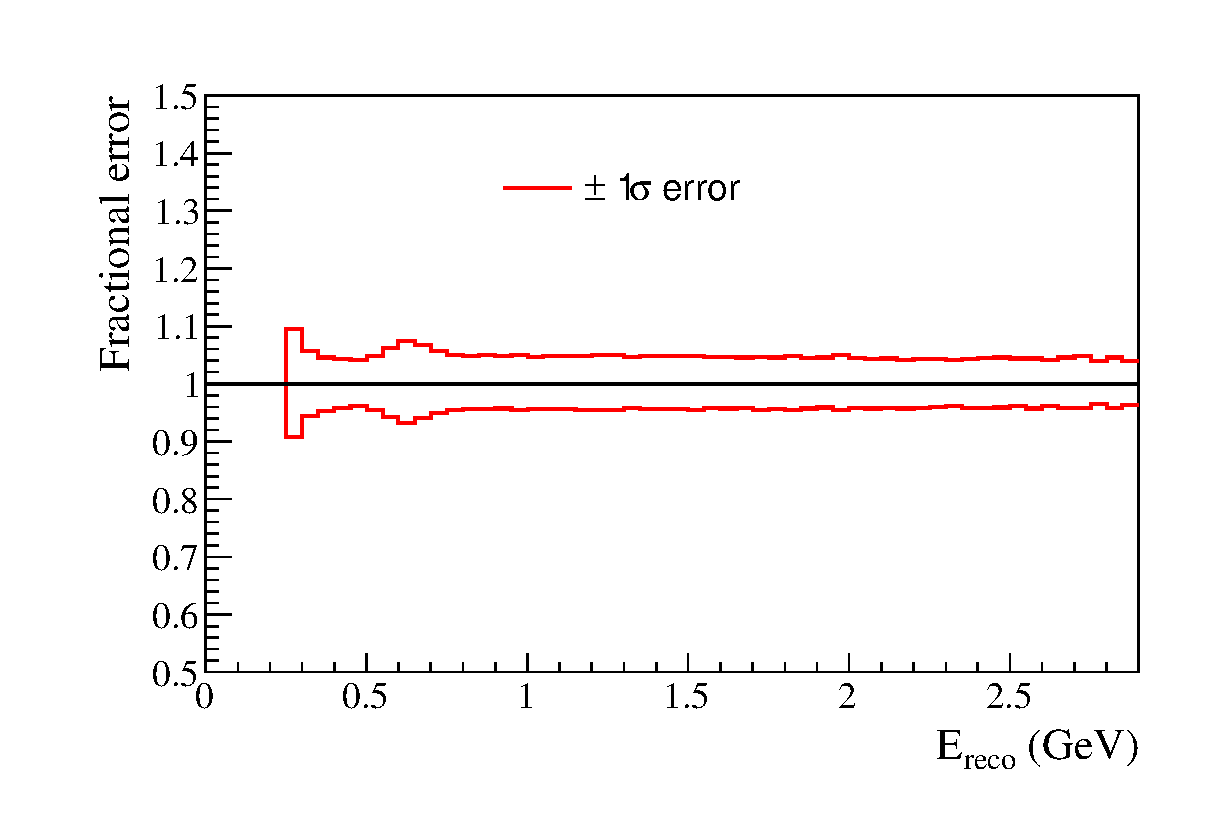
\includegraphics[width=0.9\textwidth]{joint_plots/systematics/Run17c/Asimov_A_RHC1Rmuoscillated_BANFF_xsec_envelope_ratio.eps} \\ 
\caption{Muon-like, antineutrino mode}
\end{subfigure}
%fhc e-like
\caption {
Error envelopes (left) and fractional errors (right) for the reconstructed neutrino energy spectrum
as a result of the cross section systematic parameters. 
	10k toy MC experiments are generated for the Asimov data set A shown in \cref{tab:osc_params_joint_asimov}
	with random systematic parameters, taking into account their correlations.
	Since the parameters $\delta_{CP}$, $\theta_{23}$ and $\Delta m^2_{32}$ ($\Delta m^2_{13}$) and mass hierarchy
will be measured,
only the uncertainty on 
$\sin^2 \theta_{13}$,
$\sin^2 \theta_{12}$
and 
$\Delta m^2_{21}$ 
are taken into account.
BANFF tuned MC templates are used. 
The distributions correspond to the collected statistics in the full Run 1-7c data set.
The changes due to the Run 1-7c flux and covariance matrix updates are applied.
}
\label{fig:xsec_envelope_Asimov_A_run17c_mulike}
\end{figure*}


\begin{figure*}[htb]
\center

\begin{subfigure}[b]{0.49\textwidth} \centering
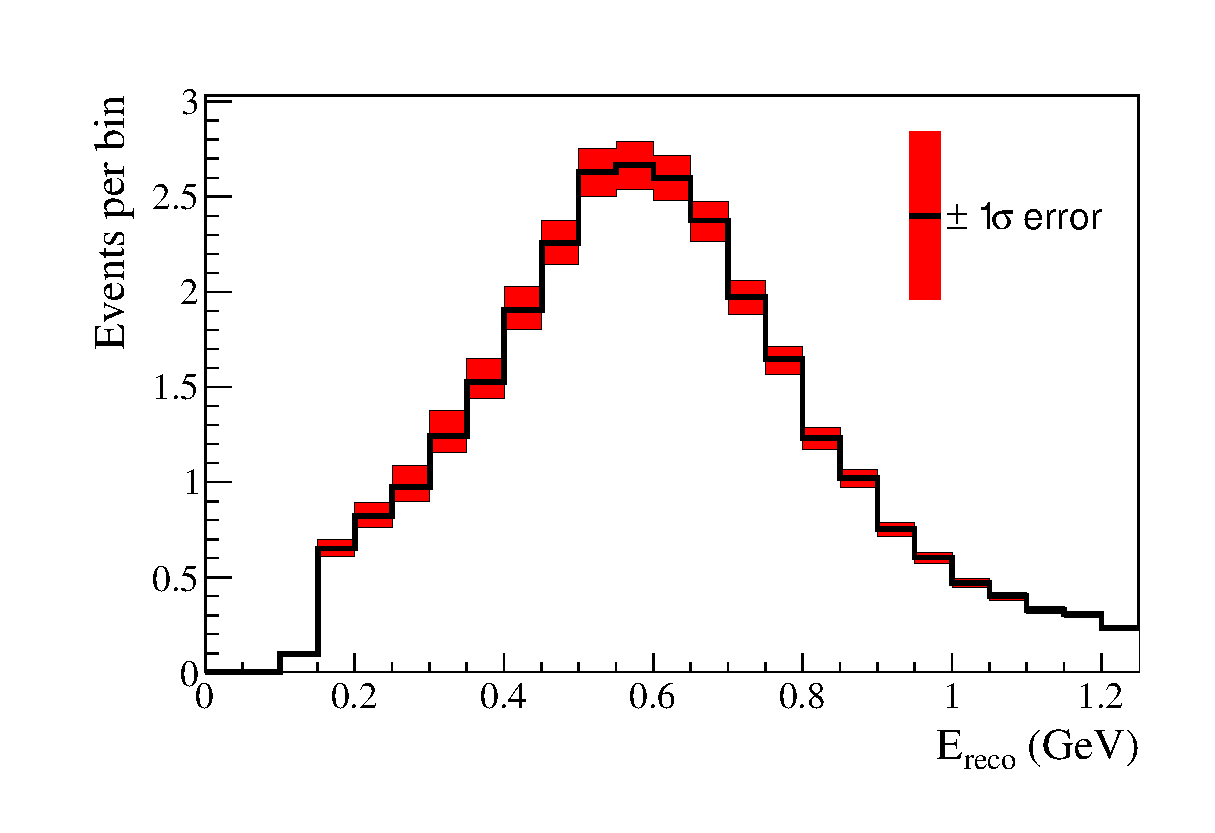
\includegraphics[width=0.9\textwidth]{joint_plots/systematics/Run17c/Asimov_A_1Reoscillated_BANFF_xsec_envelope.eps} 
\caption{Electron-like, neutrino mode}
\end{subfigure}
\begin{subfigure}[b]{0.49\textwidth} \centering
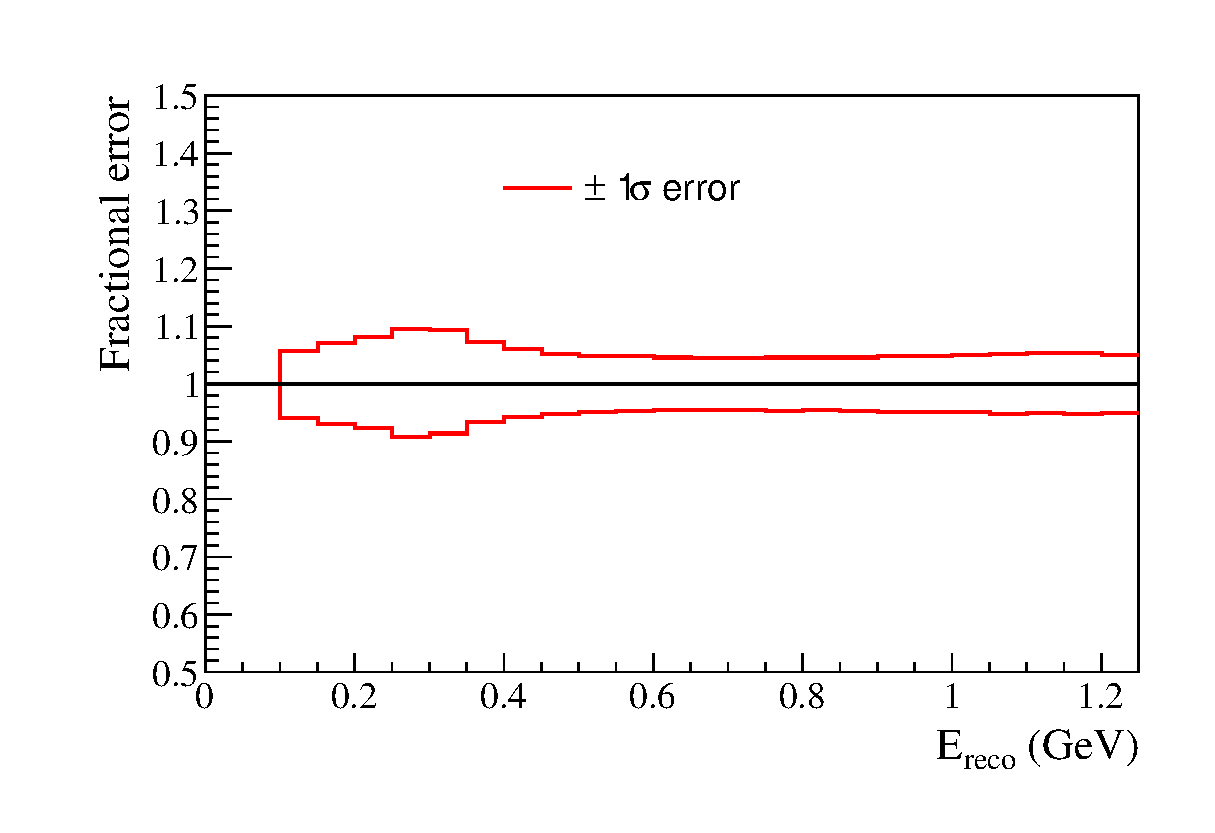
\includegraphics[width=0.9\textwidth]{joint_plots/systematics/Run17c/Asimov_A_1Reoscillated_BANFF_xsec_envelope_ratio.eps} 
\caption{Electron-like, neutrino mode}
\end{subfigure}
%rhc e-like
\begin{subfigure}[b]{0.49\textwidth} \centering
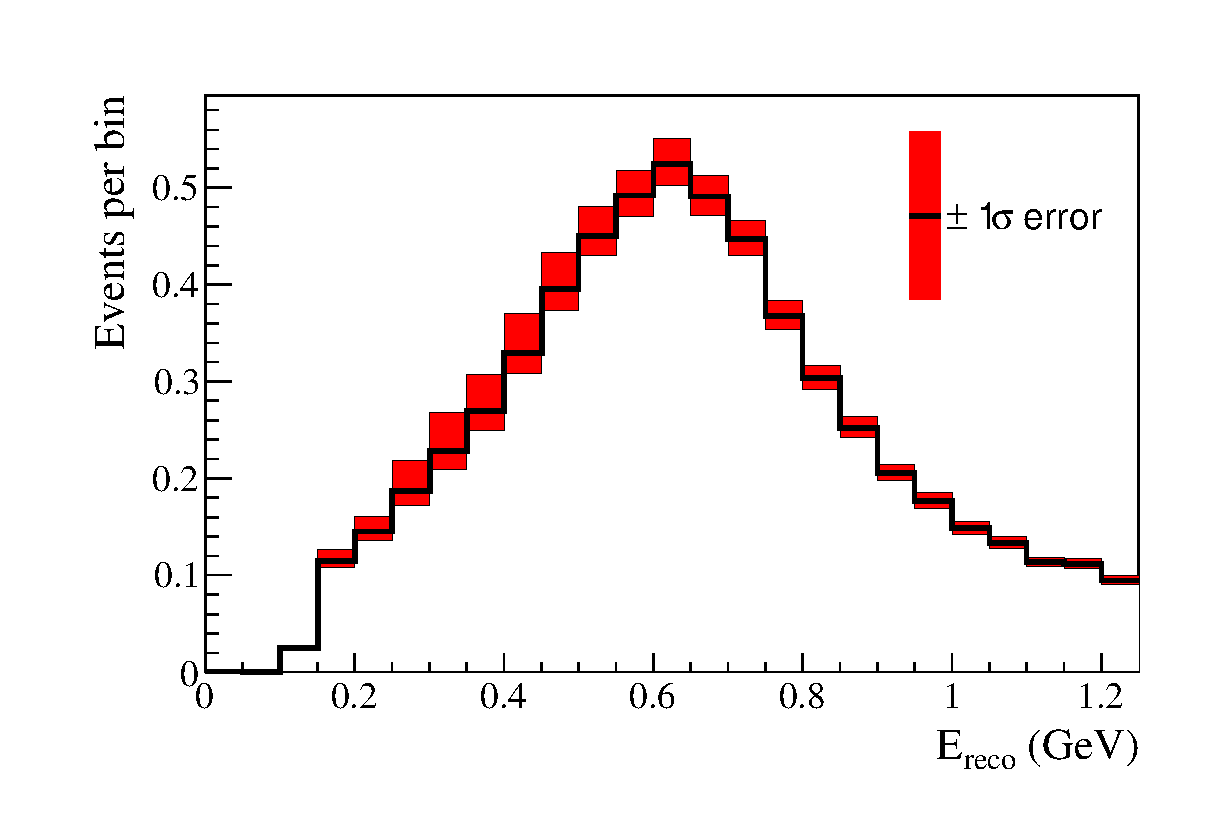
\includegraphics[width=0.9\textwidth]{joint_plots/systematics/Run17c/Asimov_A_RHC1Reoscillated_BANFF_xsec_envelope.eps} 
\caption{Electron-like, antineutrino mode}
\end{subfigure}
\begin{subfigure}[b]{0.49\textwidth} \centering
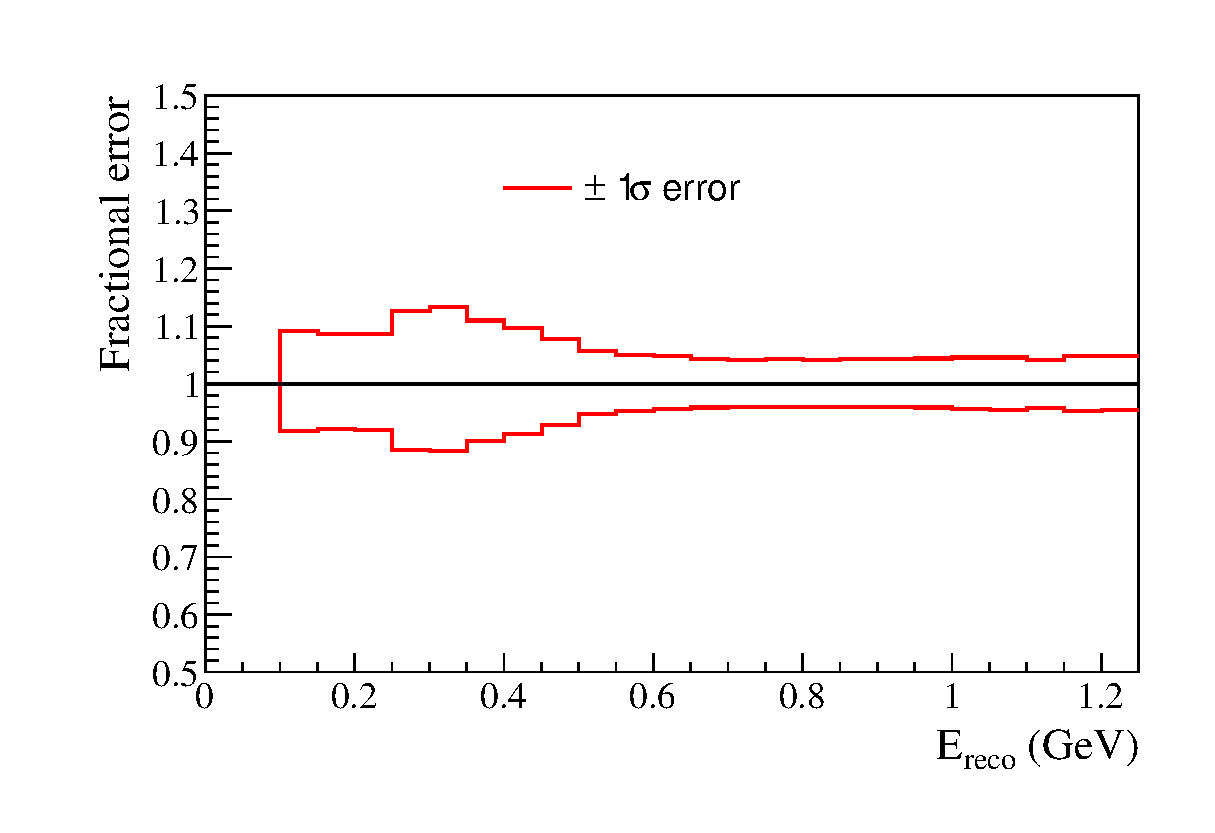
\includegraphics[width=0.9\textwidth]{joint_plots/systematics/Run17c/Asimov_A_RHC1Reoscillated_BANFF_xsec_envelope_ratio.eps} 
\caption{Electron-like, antineutrino mode}
%fhc ccpi-like
\begin{subfigure}[b]{0.49\textwidth} \centering
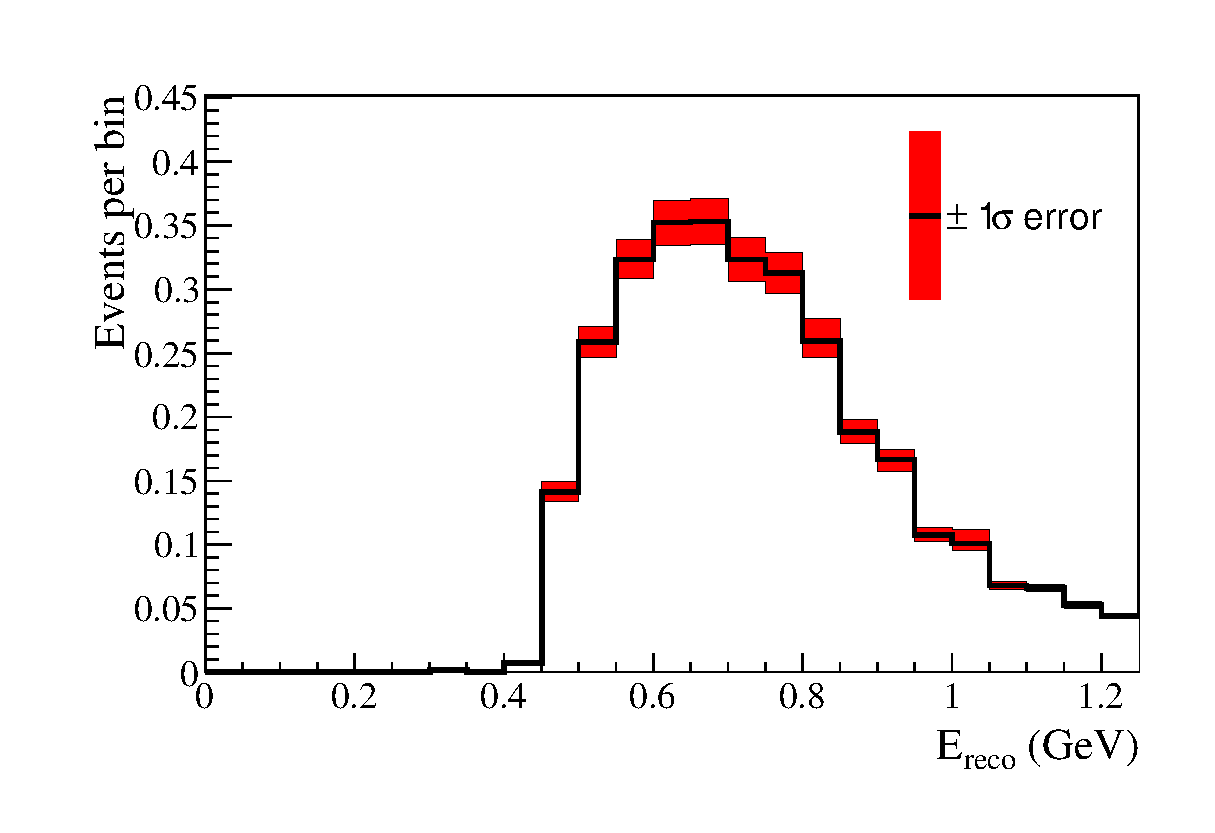
\includegraphics[width=0.9\textwidth]{joint_plots/systematics/Run17c/Asimov_A_MultiReoscillated_BANFF_xsec_envelope.eps} 
\caption{\nueCConepi{}, neutrino mode}
\end{subfigure}
\begin{subfigure}[b]{0.49\textwidth} \centering
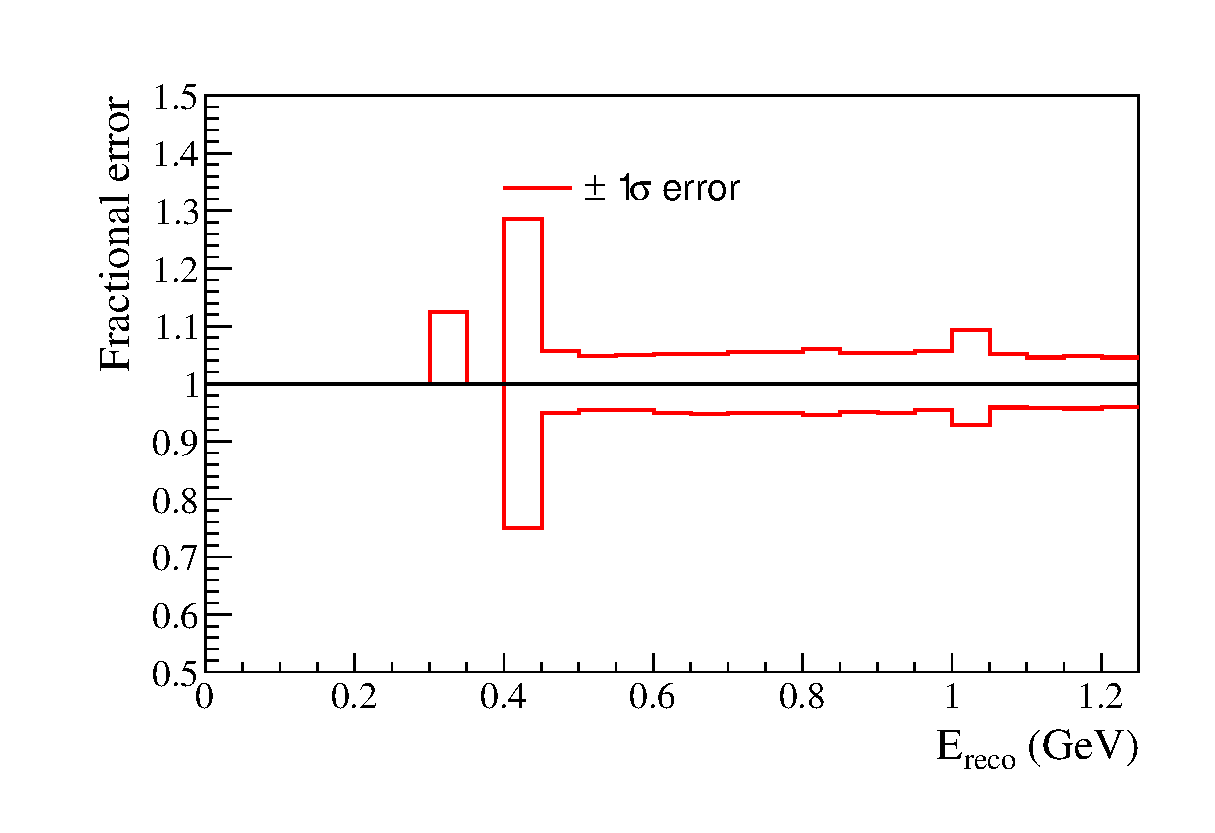
\includegraphics[width=0.9\textwidth]{joint_plots/systematics/Run17c/Asimov_A_MultiReoscillated_BANFF_xsec_envelope_ratio.eps} 
\caption{\nueCConepi{}, neutrino mode}
\end{subfigure}
\end{subfigure}
\caption {
Error envelopes (left) and fractional errors (right) for the reconstructed neutrino energy spectrum
as a result of the cross section systematic parameters. 
10k toy MC experiments are generated for the Asimov data set A shown in \cref{tab:osc_params_joint_asimov}
with randomised systematic parameters, taking into account their correlations.
Since the parameters $\delta_{CP}$, $\theta_{23}$ and $\Delta m^2_{32}$ ($\Delta m^2_{13}$) and mass hierarchy
will be measured,
only the uncertainty on 
$\sin^2 \theta_{13}$,
$\sin^2 \theta_{12}$
and 
$\Delta m^2_{21}$ 
are taken into account.
BANFF tuned MC templates are used. 
The distributions correspond to the collected statistics in the full Run 1-7c data set.
The changes due to the Run 1-7c flux and covariance matrix updates are applied.
}
\label{fig:xsec_envelope_Asimov_A_run17c_elike}
\end{figure*}


\begin{figure*}[htb]
\center
%fhc mu-like
\begin{subfigure}[b]{0.49\textwidth} \centering
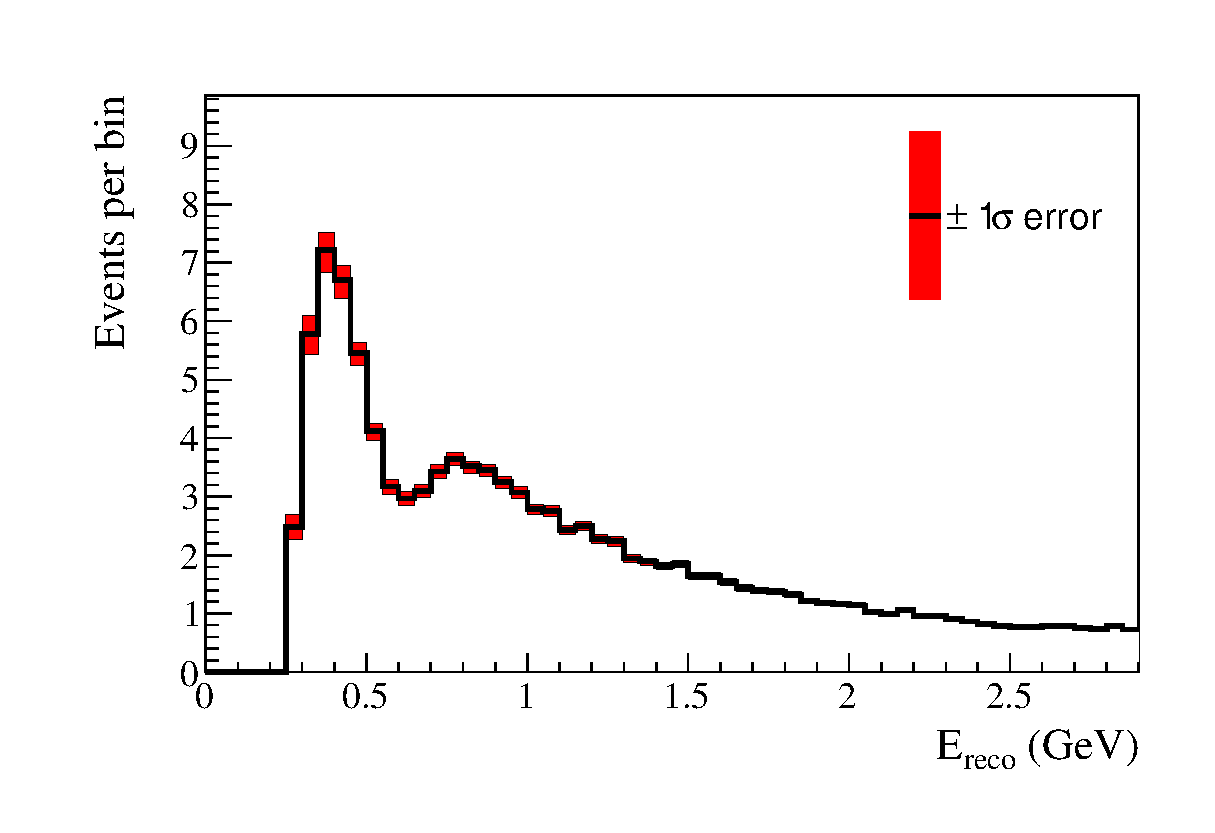
\includegraphics[width=0.9\textwidth]{joint_plots/systematics/Run17c/Asimov_A_1Rmuoscillated_BANFF_envelope.eps} 
\caption{Muon-like, neutrino mode}
\end{subfigure}
\begin{subfigure}[b]{0.49\textwidth} \centering
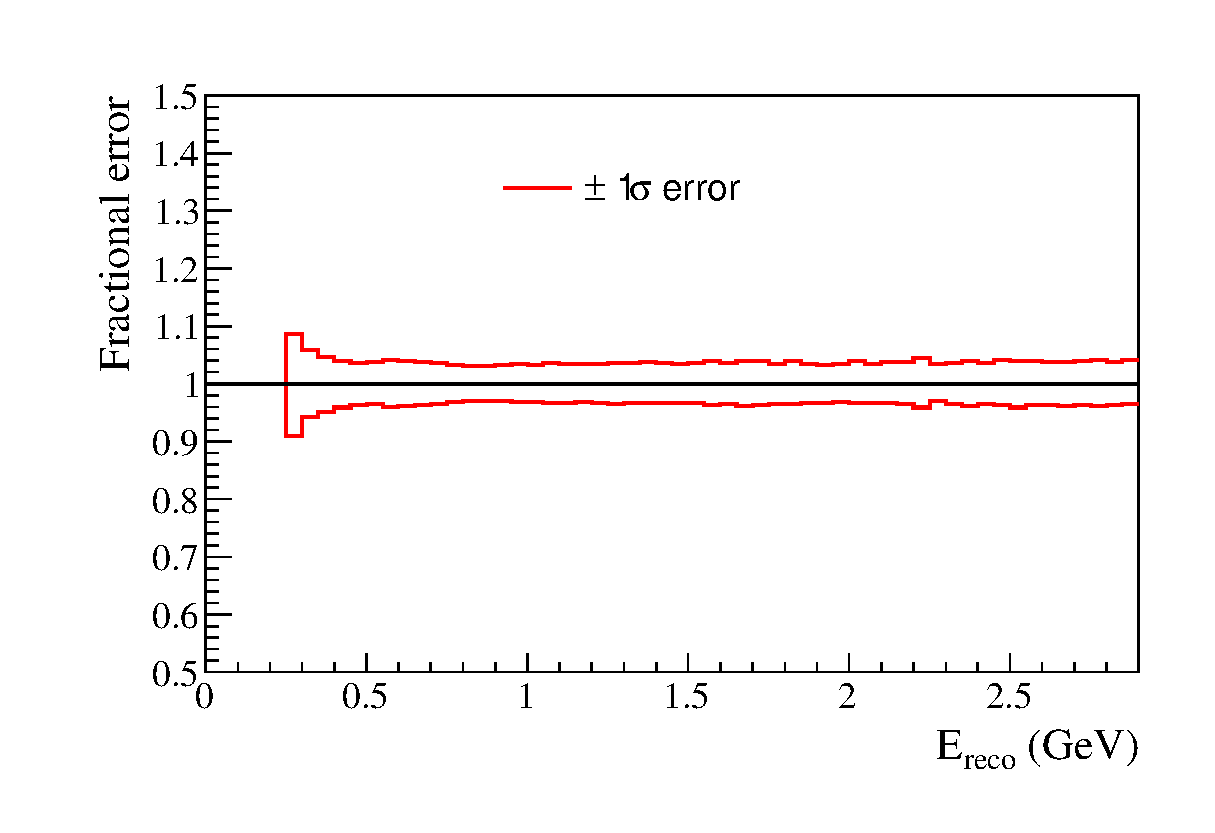
\includegraphics[width=0.9\textwidth]{joint_plots/systematics/Run17c/Asimov_A_1Rmuoscillated_BANFF_envelope_ratio.eps} 
\caption{Muon-like, neutrino mode}
\end{subfigure}
%fhc mu-like
\begin{subfigure}[b]{0.49\textwidth} \centering
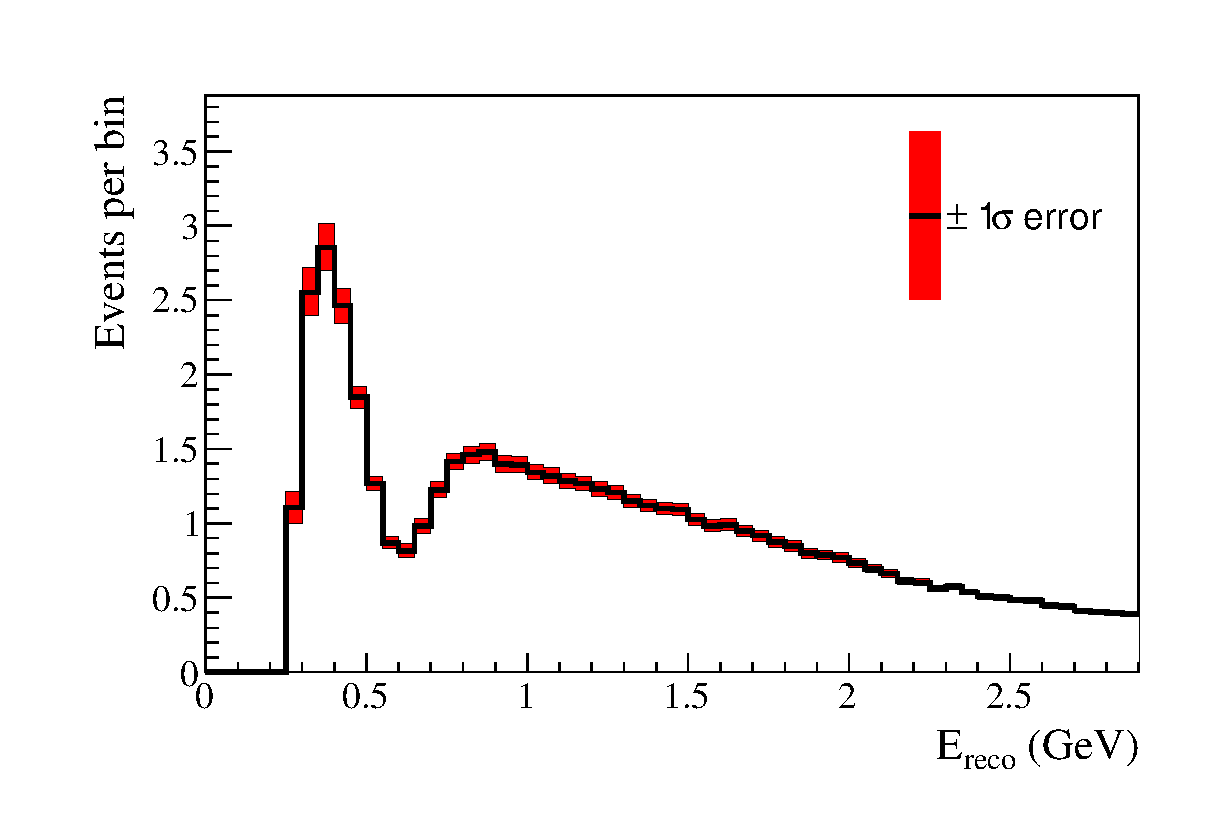
\includegraphics[width=0.9\textwidth]{joint_plots/systematics/Run17c/Asimov_A_RHC1Rmuoscillated_BANFF_envelope.eps} \\ 
\caption{Muon-like, antineutrino mode}
\end{subfigure}
\begin{subfigure}[b]{0.49\textwidth} \centering
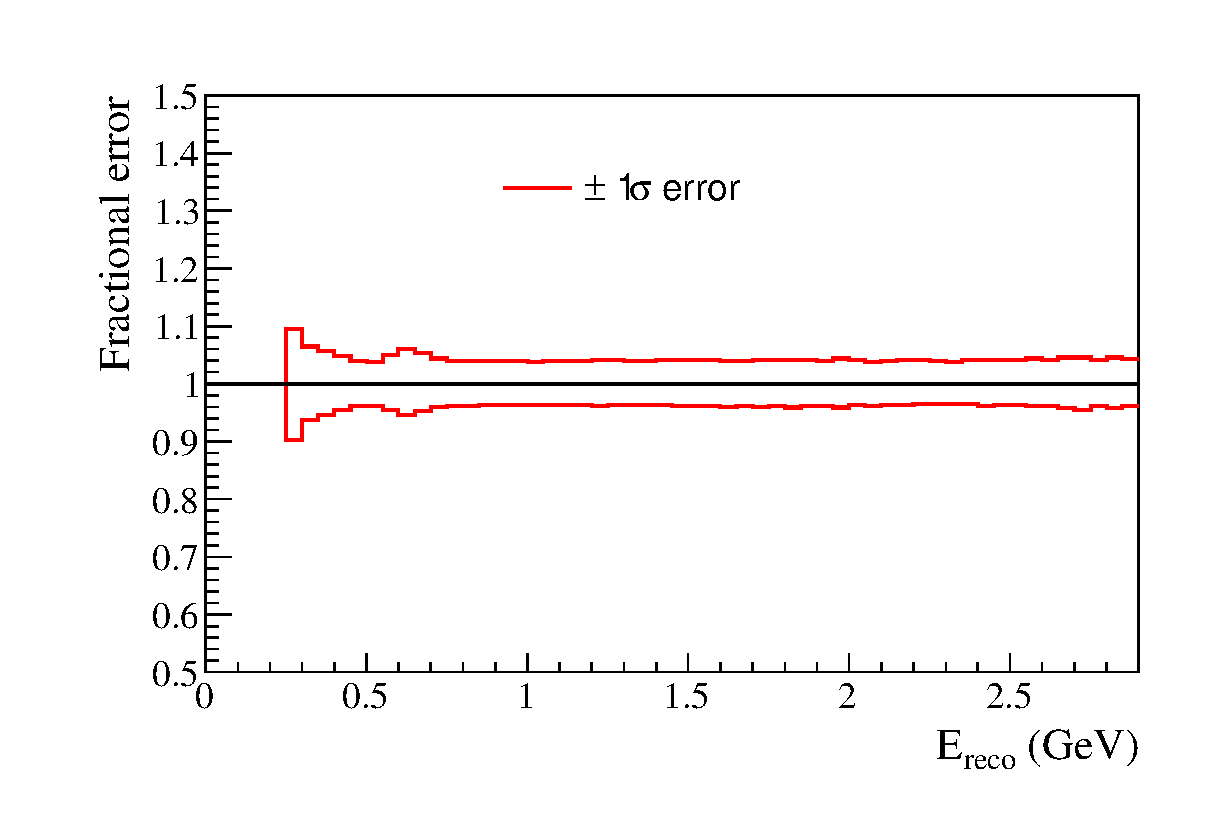
\includegraphics[width=0.9\textwidth]{joint_plots/systematics/Run17c/Asimov_A_RHC1Rmuoscillated_BANFF_envelope_ratio.eps} \\ 
\caption{Muon-like, antineutrino mode}
\end{subfigure}
%fhc mu-like
\caption {
Error envelopes (left) and fractional errors (right) for the reconstructed neutrino energy spectrum
as a result of the flux plus cross section systematic parameters. 
	10k toy MC experiments are generated for the Asimov data set A shown in \cref{tab:osc_params_joint_asimov}
	with random systematic parameters, taking into account their correlations.
	Since the parameters $\delta_{CP}$, $\theta_{23}$ and $\Delta m^2_{32}$ ($\Delta m^2_{13}$) and mass hierarchy
will be measured,
only the uncertainty on 
$\sin^2 \theta_{13}$,
$\sin^2 \theta_{12}$
and 
$\Delta m^2_{21}$ 
are taken into account.
BANFF tuned MC templates are used. 
The distributions correspond to the collected statistics in the full Run 1-7c data set.
The changes due to the Run 1-7c flux and covariance matrix updates are applied.
}
\label{fig:flux_xsec_envelope_Asimov_A_run17c_mulike}
\end{figure*}


\begin{figure*}[htb]
\center

\begin{subfigure}[b]{0.49\textwidth} \centering
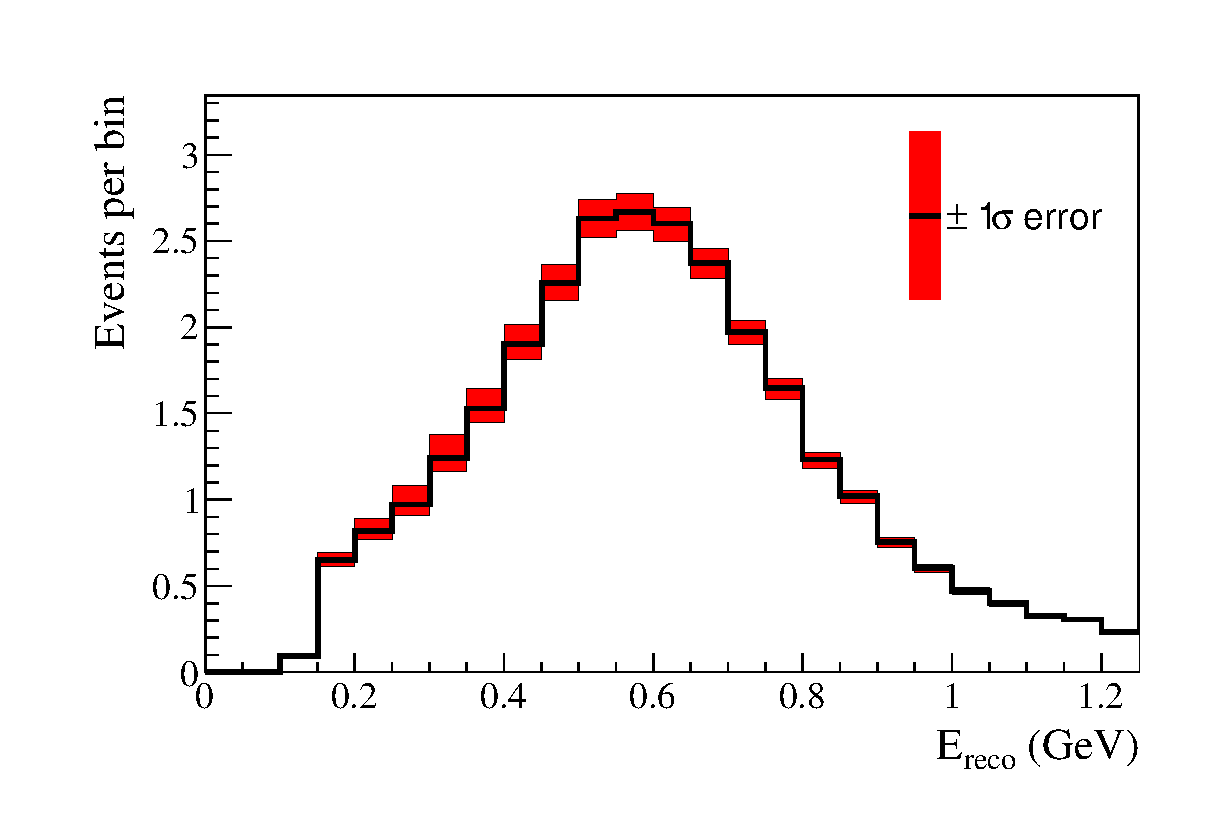
\includegraphics[width=0.9\textwidth]{joint_plots/systematics/Run17c/Asimov_A_1Reoscillated_BANFF_envelope.eps} 
\caption{Electron-like, neutrino mode}
\end{subfigure}
\begin{subfigure}[b]{0.49\textwidth} \centering
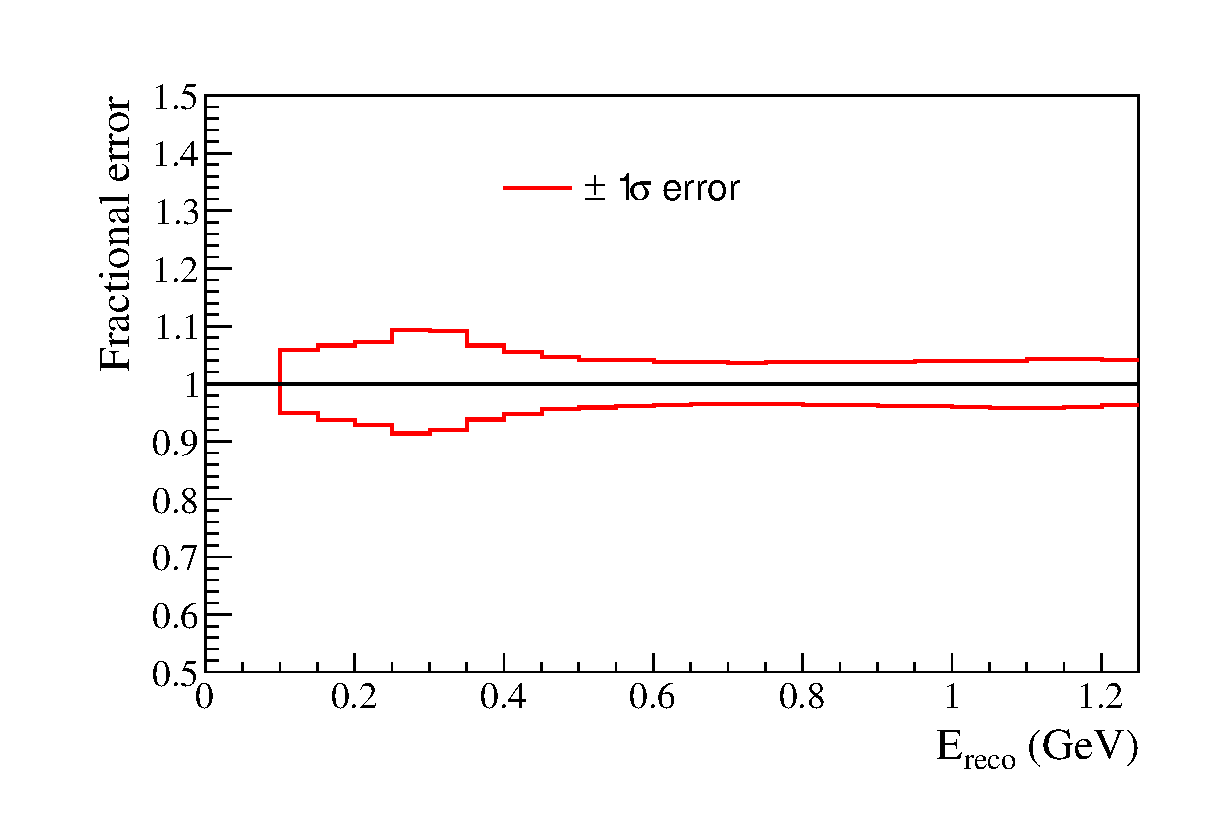
\includegraphics[width=0.9\textwidth]{joint_plots/systematics/Run17c/Asimov_A_1Reoscillated_BANFF_envelope_ratio.eps} 
\caption{Electron-like, neutrino mode}
\end{subfigure}
%fhc mu-like
\begin{subfigure}[b]{0.49\textwidth} \centering
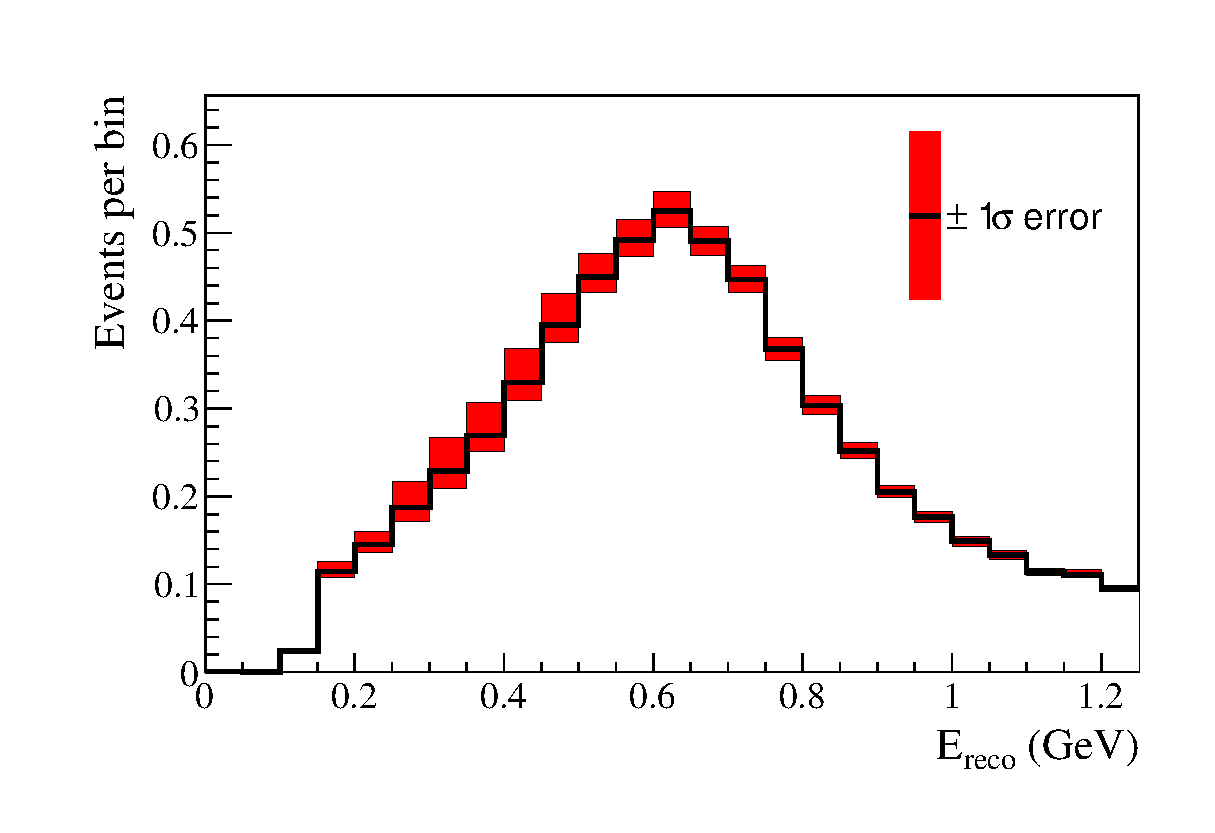
\includegraphics[width=0.9\textwidth]{joint_plots/systematics/Run17c/Asimov_A_RHC1Reoscillated_BANFF_envelope.eps} 
\caption{Electron-like, antineutrino mode}
\end{subfigure}
\begin{subfigure}[b]{0.49\textwidth} \centering
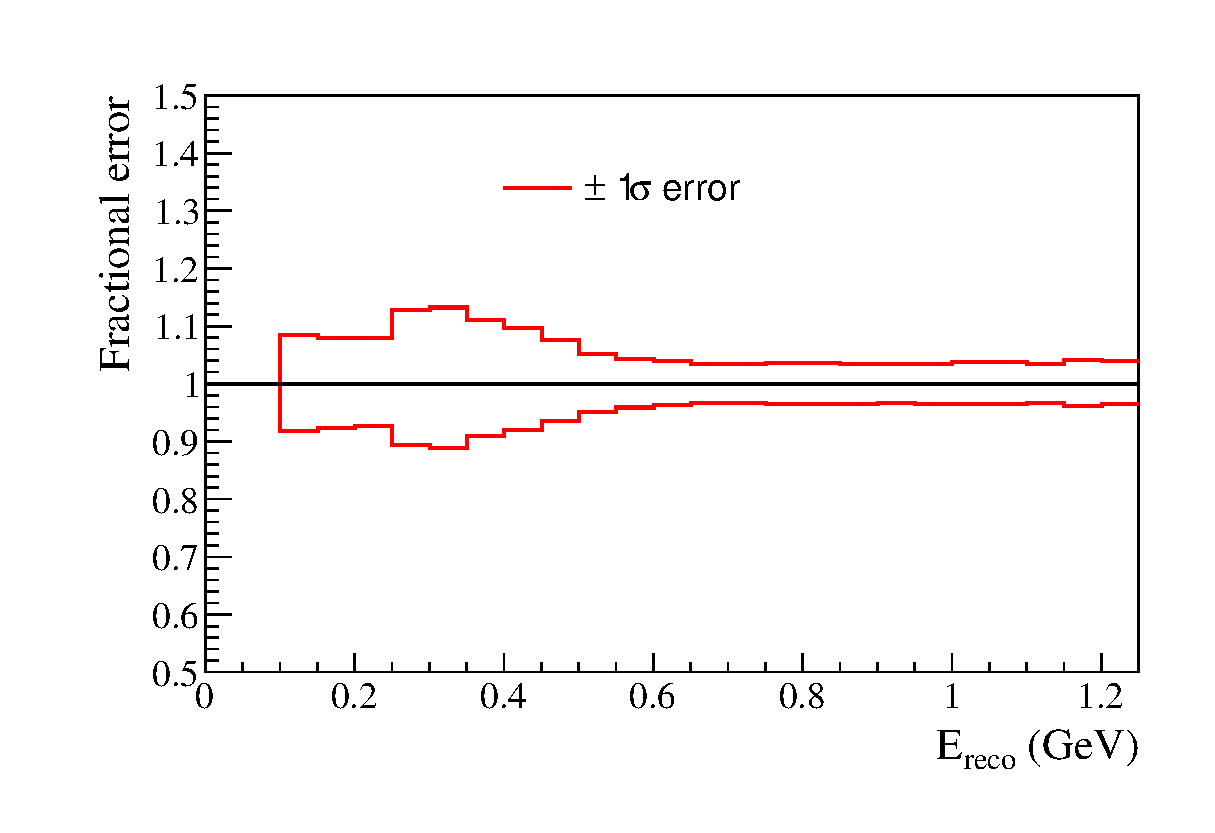
\includegraphics[width=0.9\textwidth]{joint_plots/systematics/Run17c/Asimov_A_RHC1Reoscillated_BANFF_envelope_ratio.eps} 
\caption{Electron-like, antineutrino mode}
\end{subfigure}
%fhc mu-like
\begin{subfigure}[b]{0.49\textwidth} \centering
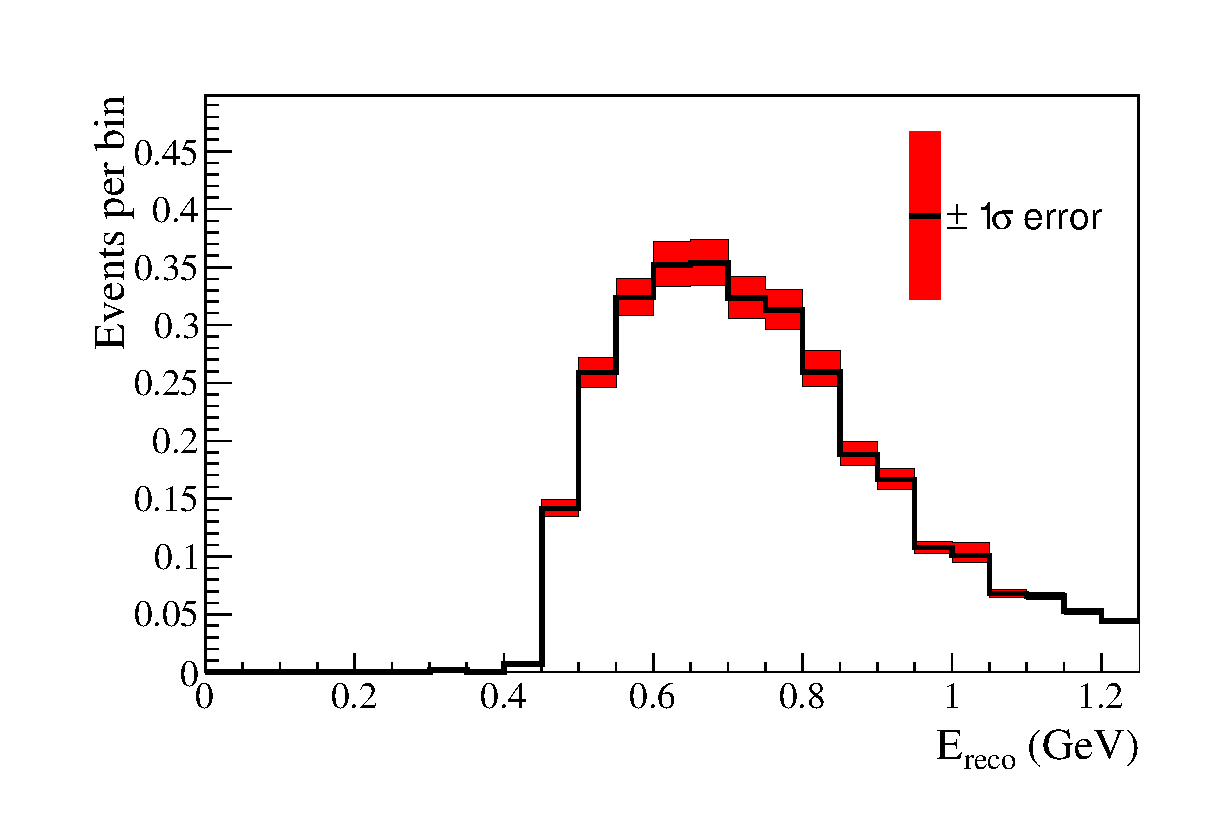
\includegraphics[width=0.9\textwidth]{joint_plots/systematics/Run17c/Asimov_A_MultiReoscillated_BANFF_envelope.eps} 
\caption{\nueCConepi{}, neutrino mode}
\end{subfigure}
\begin{subfigure}[b]{0.49\textwidth} \centering
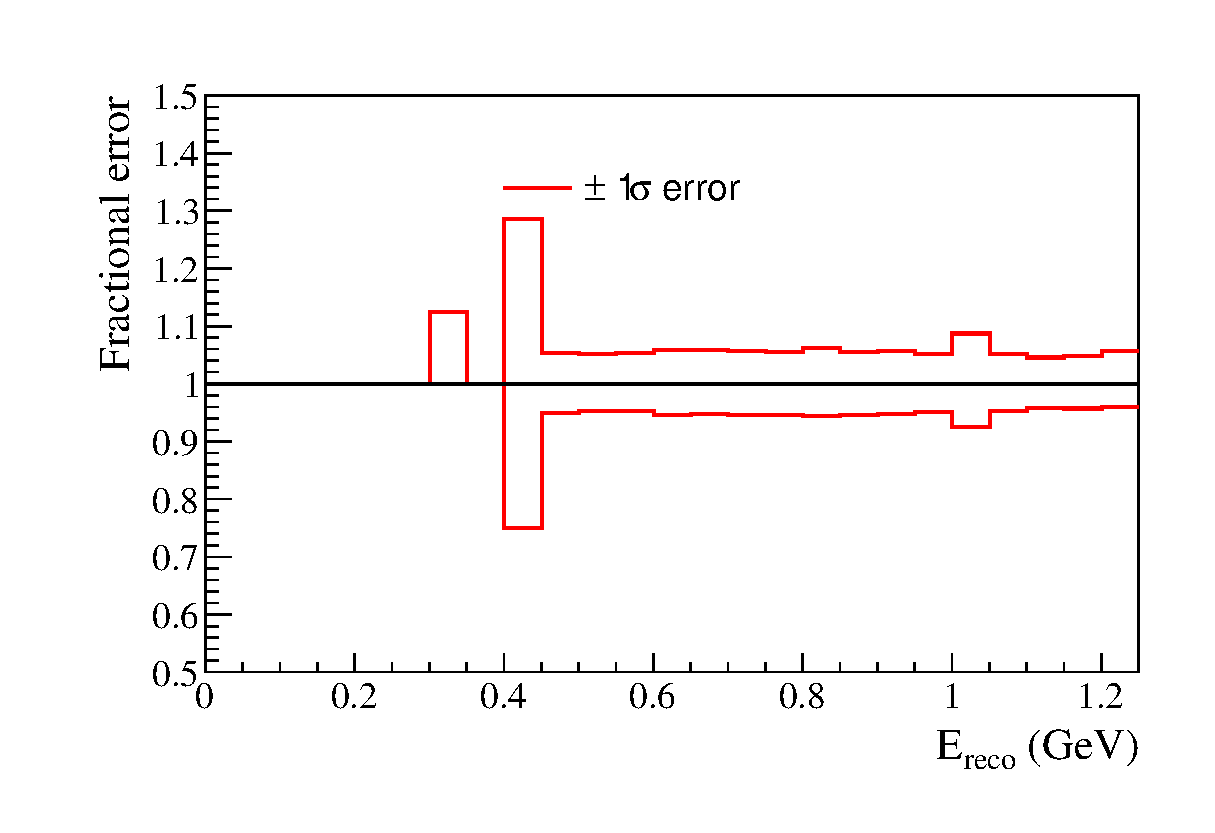
\includegraphics[width=0.9\textwidth]{joint_plots/systematics/Run17c/Asimov_A_MultiReoscillated_BANFF_envelope_ratio.eps} 
\caption{\nueCConepi{}, neutrino mode}
\end{subfigure}
\caption {
Error envelopes (left) and fractional errors (right) for the reconstructed neutrino energy spectrum
as a result of the flux plus cross section systematic parameters. 
10k toy MC experiments are generated for the Asimov data set A shown in \cref{tab:osc_params_joint_asimov}
with randomised systematic parameters, taking into account their correlations.
Since the parameters $\delta_{CP}$, $\theta_{23}$ and $\Delta m^2_{32}$ ($\Delta m^2_{13}$) and mass hierarchy
will be measured,
only the uncertainty on 
$\sin^2 \theta_{13}$,
$\sin^2 \theta_{12}$
and 
$\Delta m^2_{21}$ 
are taken into account.
BANFF tuned MC templates are used. 
The distributions correspond to the collected statistics in the full Run 1-7c data set.
The changes due to the Run 1-7c flux and covariance matrix updates are applied.
}
\label{fig:flux_xsec_envelope_Asimov_A_run17c_elike}
\end{figure*}




\clearpage














%%
%% Posterior predictive method
%%
%
%\subsection{Posterior predictive method for the choice of the prior}
%\label{sec:posterior_predictive_run17c}
%
%The posterior predictive method has been tested for the Run 1-7c statistic as well
%using the same procedure described in \cref{sec:posterior_predictive}.
%
%As shown in \cref{tab:critval_posterior_Asimov_A_run17c} and~\ref{tab:critval_posterior_Asimov_B_run17c}
%the posterior predictive critical values obtained for Asimov data sets A and B
%at $1\sigma$, 90\% and $2\sigma$ CL are similar to the prior predictive ones,
%as for the previous analyses. 
%
%\begin{figure*}[htb]
%\center
%%
\includegraphics[width=0.9\textwidth]{./images/missing_plot-eps-converted-to.pdf}
%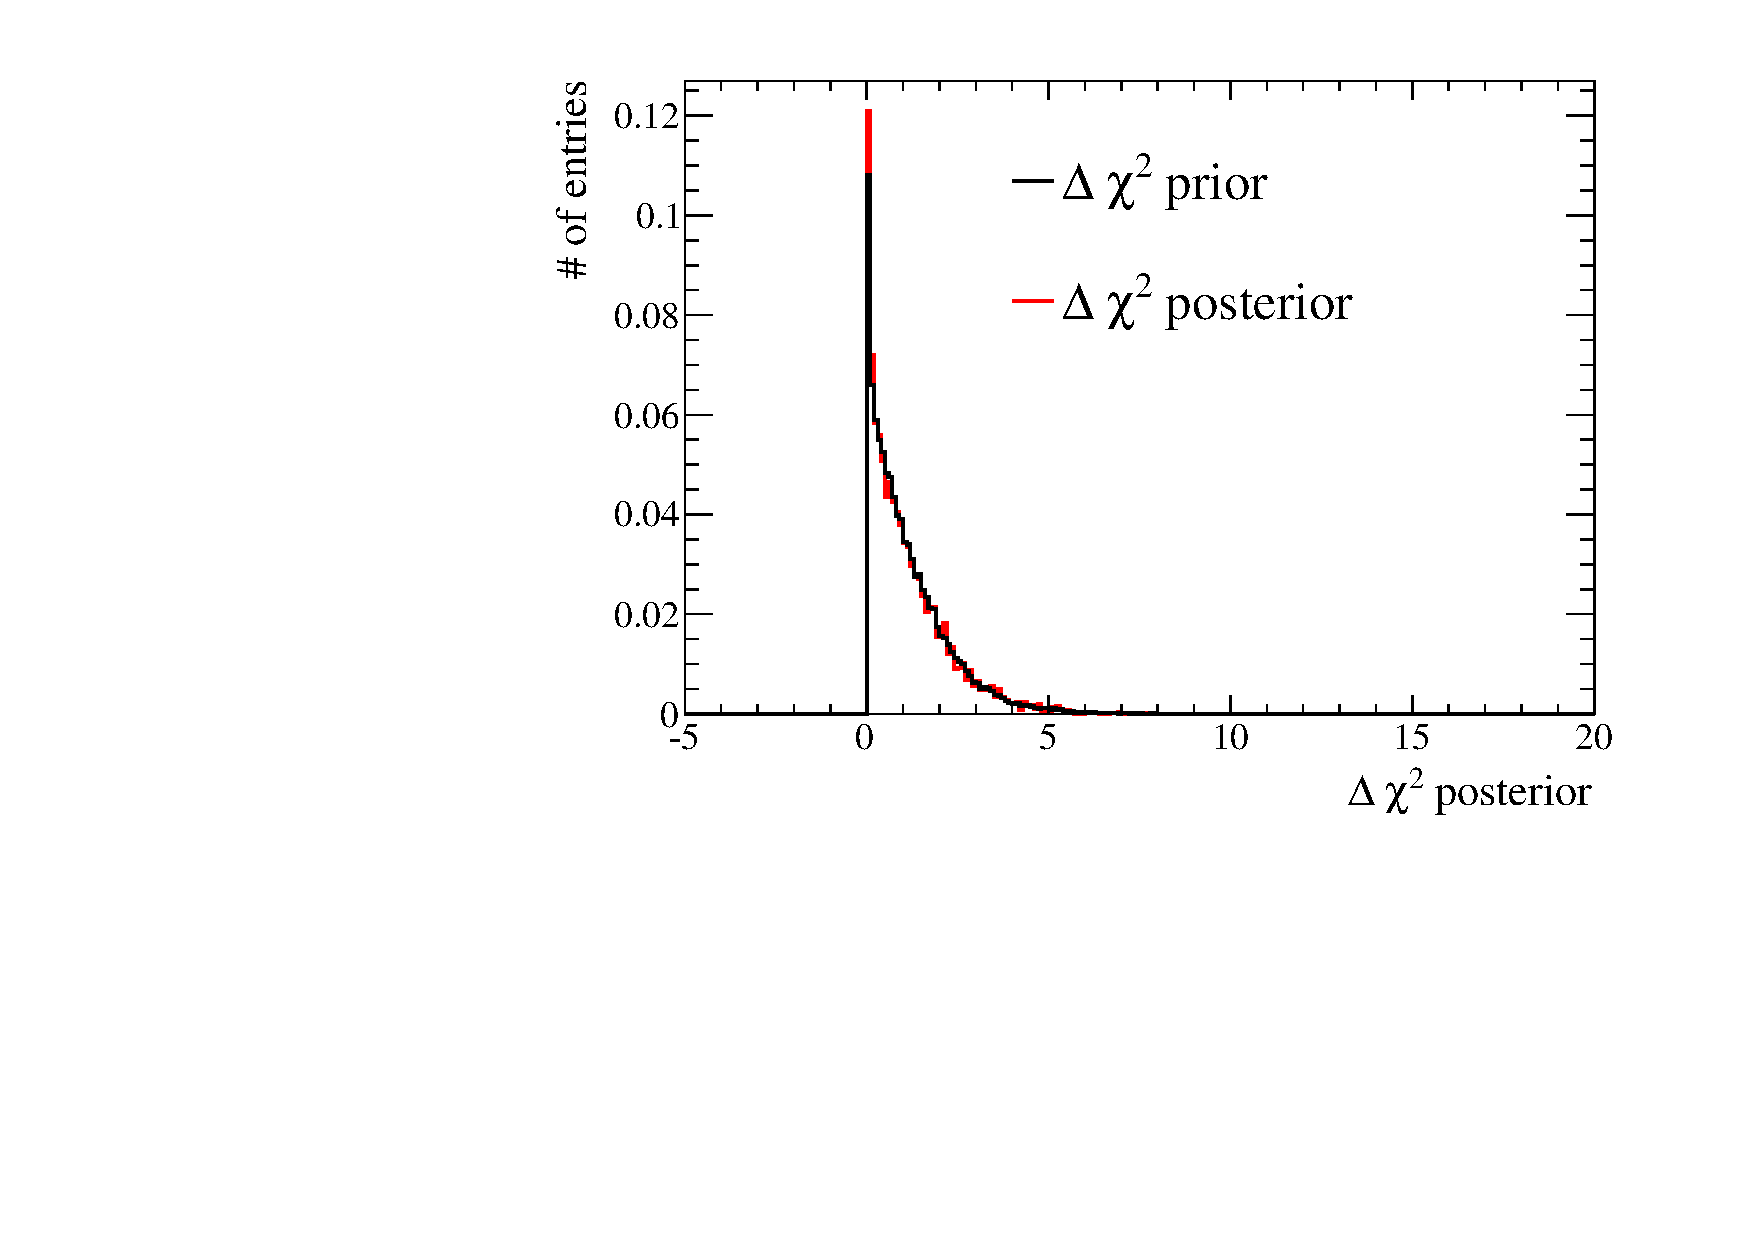
\includegraphics[width=0.49\textwidth]{./joint_plots/coverage_fc/posterior_predictive_run17c/Asimov_A/deltachisq_posterior_Asimov_A.pdf}
%\caption {
%$\Delta \chi^2$ distributions with prior (black) and posterior (red) predictive methods.
%The comparison between the two distributions normalized to 1 is shown.
%Fake data sets are generated with $\delta_{CP} = 0$ and normal hierarchy.
%The Asimov data A is used to generate the weights of the fake data sets.
%50k fake data sets are used.
%Since the posterior predictive distribution is weighted, the effective number of entries is lower with respect 
%to the prior predictive case. 
%}
%\label{fig:post_Asimov_A_dcp_0_nh_run17c}
%\end{figure*}
%
%
%\begin{table}
%\center
%\begin{tabular}{| c | c | c |}
%\hline
%{\bf CL} 				& {\bf Prior} &{\bf Posterior}  \\
%\hline
%\hline
%\multicolumn{3}{| c | }{$\delta^{true}_{CP} = 0$, $MH^{true} = \text{normal}$}  \\
%\hline
%$1\sigma$				&1.390  		& $1.360 ^{+0.024}_{-0.024}$	\\ \hline	
%90\%					&2.592  		& $2.583 ^{+0.053}_{-0.058}$	\\ \hline	
%$2\sigma$				&3.391 		& $3.413 ^{+0.078}_{-0.049}$	\\ \hline	
%\hline
%\multicolumn{3}{| c | }{$\delta^{true}_{CP} = 0$, $MH^{true} = \text{inverted}$}  \\
%\hline
%$1\sigma$				&1.356  		& $1.365 ^{+0.019}_{-0.025}$	\\ \hline	
%90\%					&2.618  		& $2.660 ^{+0.058}_{-0.040}$	\\ \hline	
%$2\sigma$				&3.430 		& $3.411 ^{+0.088}_{-0.040}$	\\ \hline	
%\hline
%\multicolumn{3}{| c | }{$\delta^{true}_{CP} = -1.351$, $MH^{true} = \text{inverted}$}  \\
%\hline
%$1\sigma$				&1.180   		& $ 1.171^{+0.021}_{-0.017}$	\\ \hline	
%90\%					&2.362		& $ 2.249^{+0.036}_{-0.042}$	\\ \hline	
%$2\sigma$				&3.306 		& $ 3.100^{+0.067}_{-0.084}$	\\ \hline	
%\end{tabular}
%\caption{
%The critical values of $\Delta \chi^2$ computed with Feldman-Cousins
%for both prior and posterior predictive method are shown.
%50k toy experiments were used. 
%%for 
%%$\delta_{CP} = 0$ and normal hierarchy
%%and
%%about 50k toy experiments were used for 
%%$\delta_{CP} = 0$ and inverted hierarchy
%%and
%%$\delta_{CP} = -1.351$ and inverted hierarchy,
%The weights of the fake data sets were generated with the Asimov data set A.
%}             
%\label{tab:critval_posterior_Asimov_A_run17c}                                                                                                                                                                             
%\end{table}
%
%
%\begin{table}
%\center
%\begin{tabular}{| c | c | c |}
%\hline
%{\bf CL} 				& {\bf Prior} &{\bf Posterior}  \\
%\hline
%\hline
%\multicolumn{3}{| c | }{$\delta^{true}_{CP} = 0$, $MH^{true} = \text{normal}$}  \\
%\hline
%$1\sigma$				& 1.390 		& $1.325 ^{+0.024}_{-0.023}$	\\ \hline	
%90\%					& 2.592 		& $2.601 ^{+0.041}_{-0.039}$	\\ \hline	
%$2\sigma$				& 3.391		& $3.448 ^{+0.045}_{-0.047}$	\\ \hline	
%\hline
%\multicolumn{3}{| c | }{$\delta^{true}_{CP} = 0$, $MH^{true} = \text{inverted}$}  \\
%\hline
%$1\sigma$				&1.356  		& $1.340 ^{+0.020}_{-0.021}$	\\ \hline	
%90\%					&2.618  		& $2.574 ^{+0.037}_{-0.032}$	\\ \hline	
%$2\sigma$				&3.430  		& $3.310 ^{+0.039}_{-0.045}$	\\ \hline	
%\hline
%\multicolumn{3}{| c | }{$\delta^{true}_{CP} = -1.351$, $MH^{true} = \text{inverted}$}  \\
%\hline
%$1\sigma$				&1.180  		& $ 1.196^{+0.014}_{-0.022}$	\\ \hline	
%90\%					& 2.362 		& $2.383 ^{+0.037}_{-0.042}$	\\ \hline	
%$2\sigma$				& 3.306		& $3.399 ^{+0.0681}_{-0.102}$	\\ \hline	
%\end{tabular}
%\caption{
%The critical values of $\Delta \chi^2$ computed with Feldman-Cousins
%for both prior and posterior predictive method are shown.
%50k toy experiments were used. 
%%for
%%$\delta_{CP} = 0$ and normal hierarchy
%%and
%%about 50k toy experiments were used for 
%%$\delta_{CP} = 0$ and inverted hierarchy
%%and
%%$\delta_{CP} = -1.351$ and inverted hierarchy,
%The weights of the fake data sets were generated with the Asimov data set B.
%}             
%\label{tab:critval_posterior_Asimov_B_run17c}                                                                                                                                                                             
%\end{table}


\clearpage




%
% Validation minimization algorithm
%



